\documentclass[openright,imperial,11pt]{octavo}

% University thesis style guide requires: A4 paper (which octavo
% doesn't quite do by default); table of contents (etc) in the table
% of contents; 1.5 line spacing; and numbered chapters.
\usepackage[BCOR=10mm,DIV=9,a4paper,pagesize]{typearea}
\usepackage{tocbibind}
\usepackage{setspace}

\onehalfspacing

\setcounter{secnumdepth}{2}
\setcounter{tocdepth}{1}

% Bibliography
\usepackage[
  citestyle=numeric-comp,
  sorting=ydnt,
  style=numeric,
]{biblatex}
\addbibresource{references.bib}

% Other packages
\usepackage[english]{babel}
\usepackage[toc]{appendix}
\usepackage[dvipsnames]{xcolor}
\usepackage{import}
\usepackage{multicol}
\usepackage{amsmath}
\usepackage{amssymb}
\usepackage{csquotes}
\usepackage{hyperref}
\hypersetup{
 colorlinks,
 citecolor=Red,
 linkcolor=Black,
 urlcolor=Blue
}

% Headings
\usepackage{titlesec}
\titleformat{\section}[hang]{\normalfont\large}{\thesection.}{1em}{}
\titleformat*{\paragraph}{\bfseries}

% Fonts
\usepackage{fontspec}
\setmainfont{equity}[
  % Files
  Path      = \string~/s/fonts/equity/ ,
  Extension = .otf ,
  % Fonts
  UprightFont     = Equity Text A Regular ,
  UprightFeatures = { SmallCapsFont = Equity Caps A Regular } ,
  BoldFont        = Equity Text A Bold ,
  BoldFeatures    = { SmallCapsFont = Equity Caps A Bold } ,
  ItalicFont      = Equity Text A Italic ,
  BoldItalicFont  = Equity Text A Bold Italic ,
  % Features
  Numbers = OldStyle ]

% Cross references
\newcommand{\partref}[1]{Part~\ref{part:#1}}
\newcommand{\chpref}[1]{Chapter~\ref{chp:#1}}
\newcommand{\secref}[1]{Section~\ref{sec:#1}}
\newcommand{\appref}[1]{Appendix~\ref{app:#1}}
\newcommand{\figref}[1]{Figure~\ref{fig:#1}}
\newcommand{\sref}[1]{(\S\ref{sec:#1})}

% Maths
\newcommand{\dependent}{\nleftrightarrow}

% Temporary
\newcommand{\todo}[1]{\emph{\color{red}{#1}}}
\usepackage{blindtext}

% Document metadata
\title{Systematic Techniques for Testing Concurrent and Distributed Functional Programs}
\author{Michael Walker}
\date{\todo{MONTH} 2018}

% Miscellaneous
\newcommand{\dejafu}{D\'{e}j\`{a}~Fu}
\newcommand{\package}[1]{\textbf{#1}}

\begin{document}
% Use roman numbering.
\frontmatter

% Disable page headings.
\pagestyle{plain}

% Avoid gaps between chapters.
\makeatletter\@openrightfalse\makeatother

\begin{titlepage}
  \begin{center}
    \makeatletter

    {\fontsize{28pt}{30pt}\selectfont \@title \par}

    \vspace{1.5cm}

    {\LARGE \@author}

    \vfill

    Submitted for the degree of\par
    Doctor of Philosophy\\[1.3cm]

    University of York\par
    Computer Science\\[1.3cm]

    \@date
    \makeatother
  \end{center}
\end{titlepage}

\chapter*{Abstract}
\addcontentsline{toc}{chapter}{Abstract}

We aim to make it easier for programmers to write correct concurrent
programs.  In pursuit of this goal, we develop three lines of work:

\paragraph{Testing concurrent Haskell}
We develop a library for testing concurrent Haskell programs using a
typeclass abstraction of concurrency.  Our tool implements
\emph{systematic concurrency testing}, a family of techniques for
deterministically testing concurrent programs.  We not only obtain a
useful tool for Haskell programs, but we also demonstrate that these
techniques work well in languages with rich concurrency abstractions.

\paragraph{Randomised concurrency testing}
We propose a new algorithm for \emph{randomly} testing concurrent
programs.  This approach is fundamentally incomplete, but is suitable
for large programs, or programs with nondeterminism beyond scheduler
nondeterminism, whereas systematic concurrency testing is not.  We
show that our algorithm performs as well as a pre-existing popular
algorithm for a standard set of benchmarks, while not requiring the
use of program-specific parameters.  We argue that this makes use and
implementation of our algorithm simpler, yet gives results which are
just as good.

\paragraph{Finding properties of programs}
We develop a tool for finding properties of sets of concurrency
functions operating on some shared state, such as the API for a
concurrent data type.  Our tool enumerates Haskell expressions and
discovers properties by comparing execution results for a variety of
inputs.  Unlike other property discovery tools, we support side
effects.  We do so by building on our tool for testing concurrent
Haskell programs.  We also generate lambda-terms, in a restricted
setting, whereas other property discovery tools typically do not.  We
argue that this approach can lead to greater understanding of
concurrency functions.

% octavo disables the "ugly" table-of-contents dots, but I find they
% improve readability.  The default dot separation is 4.5, but I like
% 7:
\makeatletter\renewcommand\@dotsep{7}\makeatother
\tableofcontents
\listoffigures
\listoftables
\listoflistings

\chapter*{Acknowledgements}
\addcontentsline{toc}{chapter}{Acknowledgements}

About a year and a half into my Ph.D, I decided that I had had enough
and wanted to quit.  I was feeling burned out over what felt like
doing the same thing over and over again, and over a conflict of
motivation I had come to recognise between myself and academia.  I am
motivated by making and maintaining tools which people use, whereas
academia is motivated by finding novel results, and the two do not
align perfectly.  Fortunately, with the encouragement of my
supervisor, I decided to give it until after the summer to set any
wheels in motion.  That break was what I needed, and I came back able
to stick it through to the end.

I did not receive any funding to do my Ph.D.  Due to the generous
support of my family, and the six months I took off for internships, I
was able to work on my Ph.D full time despite the financial handicap.
Having to self-fund a degree is a bit of a shock which forces you to
become good with money.  Even though it was hard at times---because it
was hard at times---I think this is one of the more directly valuable
skills I gained during my time.  I only wish I'd learned this as an
undergraduate, when I really didn't need to spend as much as I did.

The PLASMA group has been a constant source of fun and of knowledge,
even though I got into the habit of going into the office at strange
hours, often not overlapping much with anyone else.  Thanks to Jos\'e
for guiding me through the strange ways of being a Ph.D student in my
first year, and to Rudy and Matt for letting me bounce ideas off them.
It's a shame that with a few of us leaving in quick succession, PLASMA
is now so small.

Thanks to my friends both in-person and online, for putting up with my
venting on more than one occasion.  Finally, thanks to those who
remind me that, no matter what is going on at the moment, one should
always strive to take it easy.

\chapter*{Declaration}
\addcontentsline{toc}{chapter}{Declaration}

This work has not previously been presented for an award at this, or
any other, university.  All sources are cited in the main text and
listed in the bibliography.  Earlier versions of parts of this thesis
were published in the following papers:

\begin{enumerate}
\item Michael Walker and Colin Runciman.  \dejafu{}: A Concurrency
  Testing Library for Haskell.  In \emph{Proceedings of the 8th ACM
    SIGPLAN Symposium on Haskell}, Haskell 2015, pages 141--152.  ACM,
  2015.\nocite{walker2015}
\item Michael Walker and Colin Runciman.  Cheap Remarks about
  Concurrent Programs.  Presented at: \emph{Trends in Functional
    Programming}.  2017.\nocite{tfp-coco}
\item Michael Walker and Colin Runciman.  Cheap Remarks about
  Concurrent Programs.  Accepted for publication in: \emph{Functional
    and Logic Programming Symposium}, FLOPS 2018.  ACM,
  2018.\nocite{flops-coco}
\end{enumerate}

These papers were conceived, implemented, and written by myself with
significant input from Prof.~Runciman.  The first paper contributes to
\Cref{chp:dejafu}, the second and third to \Cref{chp:coco}.  An
updated version of the \dejafu{} paper was published as a departmental
technical report:

\begin{enumerate}
\setcounter{enumi}{3}
\item Michael Walker. \dejafu{}: A Concurrency Testing Library for
  Haskell.  Technical report, University of York, Department of
  Computer Science, 2016.\nocite{YCS-2016-503}
\end{enumerate}

The inspiration for the investigation in \Cref{chp:algorithms} arose
from discussions with Dr.~Alistair Donaldson and the now-Dr.~Paul
Thomson\footnote{Both at Imperial College London}.


\cleardoublepage

% Use arabic numbering.
\mainmatter

% Open chapters on right-side pages.
\makeatletter\@openrighttrue\makeatother

% Enable chapter headings at the top of the page.
\pagestyle{headings}

% The thesis!
\chapter{Introduction}
\label{chp:introduction}
There is a tension between theory and practice in software
engineering.  Whenever one programmer suggests some sophisticated
technique or formalism, another will question its applicability to the
\emph{real world}, a nebulous and undefined place.  Here is an
example:

\begin{description}
\item[Alice] ``If you want a reliable concurrent program, you have to
  model check your core algorithms.''
\item[Bob] ``Model checking doesn't scale to real-world concurrent
  programs, you just have to stress test them.''
\end{description}

Bob's concern is not unfounded.  While model checking can prove the
absence of bugs, it can be difficult or resource-intensive to use.
Whereas stress testing, aided by dynamic analyses like Clang's
ThreadSanitizer\footnote{\url{https://clang.llvm.org/docs/ThreadSanitizer.html}}
or Go's data race
detector\footnote{\url{https://golang.org/doc/articles/race_detector.html}},
is often effective at finding flaws.  Where testing falls down,
however, is answering questions like:

\begin{itemize}
\item How do we ensure that we're covering a variety of schedules?
\item How do we know a that bug has been fixed?
\item \emph{How much testing is enough?}
\end{itemize}

In this thesis, we follow a middle path: between the familiarity of
testing and the power of model checking.  By leveraging
\emph{systematic concurrency testing}, we enable programmers to test
their concurrent programs deterministically, and confidently.

We use Haskell is used in this thesis.  \Cref{app:haskell} gives a
brief introduction to Haskell for the reader already somewhat familiar
with functional programming.

\section{Parallelism vs Concurrency}
\label{sec:intro-parconc}

In many fields, `parallelism' and `concurrency' are synonyms, both
referring to doing multiple things at once.  In programming, they
refer to different but related concepts.

\paragraph{Parallelism}
A parallel program uses a multiplicity of hardware to compute
different aspects of a result simultaneously.  The goal is to arrive
at the overall result more quickly.  For example, the x86 assembly
instruction \verb#PMULHUW# computes the element-wise multiplication of
two vectors, performing each multiplication simultaneously: it enables
parallelism.

\paragraph{Concurrency}
A concurrent program uses a notion of multiple threads of control to
structure the program.  These threads conceptually execute
independently and the same time.  Whether threads actually do execute
simultaneously is an implementation detail.  A concurrent program can
execute on a single-core machine through interleaved sequential
execution just as it can execute on a multi-core machine in parallel.
A concurrency abstraction can guarantee parallelism (given suitable
hardware), for example by having the ability to restrict the execution
of individual threads to given processor cores.

This thesis is concerned with concurrency, but parallelism does rear
its head in the discussion of \emph{relaxed memory} in
\Cref{chp:dejafu}.

\section{Goals and Contributions of this Thesis}
\label{sec:intro-contributions}

The primary contribution of this thesis is to demonstrate that
concurrency testing techniques, typically described in the context of
a simple core language, can be successfully applied to languages with
rich concurrency abstractions.  This demonstration is in the form of a
library for testing concurrent Haskell programs.

Our contributions are:

\begin{itemize}
\item A library for effectively testing concurrent Haskell programs.
\item A convincing demonstration that concurrency testing techniques
  work well in a rich setting.
\item A new scheduling algorithm for randomised testing.
\item A tool for discovering properties of concurrent Haskell
  functions.
\end{itemize}

The overall motivation of this research has been to develop tools
which make it easier for programmers to write correct concurrent
programs.

\section{Roadmap}
\label{sec:intro-roadmap}

This thesis is divided into three parts:

\paragraph{\Cref{part:review}}
We present the context and background of the work.
\Cref{chp:concurrent_haskell} gives an introduction to concurrency in
Haskell.  \Cref{chp:sct} discusses the theory behind \emph{testing}
concurrent programs.  Finally, \Cref{chp:property_testing} gives an
introduction to property testing in Haskell.

\paragraph{\Cref{part:testing}}
We present our contributions.  \Cref{chp:dejafu} gives an account of
the \dejafu{} tool for testing concurrent Haskell programs, covering
the scope, implementation, and some case studies.
\Cref{chp:algorithms} discusses an alternative scheduling algorithm
for testing concurrent programs.  Finally, \Cref{chp:coco} gives an
account of the CoCo tool for discovering properties of concurrent
Haskell programs, covering the scope, implementation, some case
studies, and shows how it connects to \dejafu{}.

\paragraph{\Cref{part:end}}
We evaluate the work and discuss our conclusions in
\Cref{chp:conclusions} and suggest possible future work in
\Cref{chp:future_work}.


\part{Background and Review}
\label{part:review}

\chapter{Concurrent Haskell}
\label{chp:concurrent_haskell}
Concurrency is not in standard Haskell, so here we restrict our
interest to GHC\@.  In this chapter we give an overview of the
concurrency functionality we use.  These operations are available in
the \package{concurrency} library.  We cover the basic use of
concurrency~\sref{concurrent_haskell-threads}, the memory
model~\sref{concurrent_haskell-mmodel}, software transactional
memory~\sref{concurrent_haskell-stm}, and finally
exceptions~\sref{concurrent_haskell-exc}.

Throughout, we compare with the concurrency abstractions of Java and
Rust.  Java because it is a popular language which, like Haskell, has
exceptions.  Rust because its design borrows from the spirit of
functional languages.

\section{Multithreading}
\label{sec:concurrent_haskell-threads}

Threads let a program do multiple things at once.  Every program has
at least one thread, which runs the main action of the program.  A
thread is the basic unit of concurrency.  It lets us pretend that
we're computing multiple things at once.

\begin{listing}
\centering
\begin{cminted}{haskell}
forkIO     :: IO () -> IO ThreadId
myThreadId :: IO ThreadId
\end{cminted}
\caption{Basic threading operations in Haskell.}\label{lst:basic_haskell}
\end{listing}

A thread can be started using the \verb|forkIO| function, which starts
executing its argument in a separate thread and also gives us back a
\verb|ThreadId| value, which can be used to kill the thread.  A thread
can get its own \verb|ThreadId| using \verb|myThreadId|.

% [layout hack]: avoid the first line (and nothing else) of the
% following paragraph from ending up on this page.
\pagebreak

\begin{listing}
\centering
\begin{cminted}{java}
/* forkIO */
Runnable runnable = /* action */;
Thread thread = new Thread(runnable);
thread.start();

/* myThreadId */
Thread me = Thread.currentThread();
\end{cminted}
\caption{Basic threading operations in Java.}\label{lst:basic_java}
\end{listing}

In Java, threads are created from classes implementing the
\verb|Runnable| interface.  The \verb|Thread| constructor creates a
new thread object from a \verb|Runnable|, but it does not start until
\verb|Thread.start| is called.  The thread object itself fulfils the
role of the Haskell \verb|ThreadId| type.  A thread can get a
reference to itself with the \verb|Thread.currentThread| static
method.

\begin{listing}
\centering
\begin{cminted}{rust}
/* forkIO */
let thread = thread::spawn(/* closure */);

/* Java-style */
let thread = thread::Builder::new().spawn(/* closure */);

/* myThreadId */
let me = thread::current();
\end{cminted}
\caption{Basic threading operations in Rust.}\label{lst:basic_rust}
\end{listing}

Rust supports both the Haskell and Java thread creation styles.  The
Haskell-style \verb|thread::spawn| function takes a closure to
execute, creates and immediately begins executing a thread, and
returns an identifier.  The alternative Java-style
\verb|thread::Builder| interface allows creating a thread without
starting it.  In both cases, the compiler gives an error if the
closure captures a variable from its outer scope without the
appropriate move semantics.

\paragraph{Capabilities}
In a real machine, there are multiple processors and cores.  It may be that a
particular application of concurrency is only a net gain if every thread is
operating on a separate core, so that threads are not interrupting each other.
GHC uses a \emph{green threading} model, where Haskell threads are multiplexed
onto a much smaller number of operating system threads.  The number of operating
system threads is referred to as the number of \emph{capabilities} or
\emph{Haskell execution contexts}.  Only operating system threads have the
possibility of executing truly in parallel.

% [layout hack]: avoid the first line (and nothing else) of the
% following paragraph from ending up on this page.
\pagebreak

\begin{listing}
\centering
\begin{cminted}{haskell}
forkOn             :: Int -> IO () -> IO ThreadId

getNumCapabilities :: IO Int
setNumCapabilities :: Int -> IO ()
\end{cminted}
\caption{Operating system threads in Haskell.}\label{lst:caps_haskell}
\end{listing}

We can fork a thread to run on a particular capability with the
\verb|forkOn| function, which takes a number identifying the
capability to use.  This capability number is interpreted modulo the
total number of capabilities, which can be queried and set.

Neither Java nor Rust provide green threading.  Java does not specify
how its threads are mapped to OS threads but, on Linux, each Java
thread is an OS thread.  Rust specifies that its threads are OS
threads.

\paragraph{Scheduling}
The GHC scheduler is good, but sometimes we have domain knowledge
which lets us do better.

\begin{listing}
\centering
\begin{cminted}{haskell}
yield       :: IO ()
threadDelay :: Int -> IO ()
\end{cminted}
\caption{Controlling thread scheduling in Haskell.}\label{lst:schedule_haskell}
\end{listing}

There are two ways to influence how threads are scheduled: we can
yield control to another thread, or delay the current thread for a
period of time.

\begin{listing}
\centering
\begin{cminted}{java}
Thread thread = /* ... */;
thread.setPriority(/* new priority */);
\end{cminted}
\caption{Thread priority in Java.}\label{lst:schedule_java}
\end{listing}

In Java, we can use the \verb|Thread.yield| and \verb|Thread.sleep|
methods to affect scheduling.  We can also adjust the \emph{priority}
of a thread, where the initial priority is inherited from its creator.
Threads with higher priority are executed in preference to threads
with lower priority:

\begin{listing}[h!]
\centering
\begin{cminted}{rust}
thread::park() /* execution stops now */

/* from another thread */
reference_to_thread::unpark();
\end{cminted}
\caption{Thread parking and unparking in Rust.}\label{lst:schedule_rust}
\end{listing}

Rust has three ways to control scheduling.  In addition to yielding
and delaying, it can also \emph{park} the current thread.  When
parked, a thread will not execute until it is unparked by another
thread.  There is a variant of \verb|thread::park| with a timeout,
which provides a delay-unless-woken construct.  Haskell threads have
no notion of priority or parking.

\paragraph{Termination}
Both Java and Rust can use a thread handle to block until that thread
terminates.  This is called \emph{joining}.  Haskell provides no join
operation.

\section{Shared State and the Memory Model}
\label{sec:concurrent_haskell-mmodel}

There are two main types of shared variable in GHC Haskell, with different
semantics.

\paragraph{Shared mutable references}
An \verb|IORef| is a mutable location in memory holding a Haskell
value.

\begin{listing}
\centering
\begin{cminted}{haskell}
newIORef   :: a -> IO (IORef a)
readIORef  :: IORef a -> IO a
writeIORef :: IORef a -> a -> IO ()
\end{cminted}
\caption{Shared mutable references in Haskell.}\label{lst:smref_haskell}
\end{listing}

As Java is an impure language with no restriction on sharing, it has
no need for a type like \verb|IORef|.  Any thread can mutate any
reference that is in scope.  Rust does impose restrictions on
mutability and sharing, and provides a few different shared variable
types.  The closest to \verb|IORef| is a reference-counting box
containing an atomically modifiable pointer.

\begin{listing}
\centering
\begin{cminted}{rust}
let ptr = &mut /* initial value */;
let shared = Arc::new(AtomicPtr::new(ptr));

let shared_clone = shared.clone();
let thread = thread::spawn(move|| {
    shared_clone.store(/* new value */, Ordering::SeqCst);
});
\end{cminted}
\caption{Shared mutable references in Rust.}\label{lst:smref_rust}
\end{listing}

Threads can modify the pointer by cloning the shared \verb|Arc| value,
extracting the inner \verb|AtomicPtr|, and updating the value inside.
All mutation operations take as a parameter the type of memory
consistency to enforce, which we shall discuss shortly.

\paragraph{Shared references under mutual exclusion}
An \verb|MVar| is a mutable location in memory with two possible
states: \emph{full}, holding a Haskell value, and \emph{empty},
holding no value.  An \verb|MVar| can be created in either state.

\begin{listing}
\centering
\begin{cminted}{haskell}
newMVar      :: a -> IO (MVar a)
newEmptyMVar :: IO (MVar a)

putMVar      :: MVar a -> a -> IO ()
readMVar     :: MVar a -> IO a
takeMVar     :: MVar a -> IO a

tryPutMVar   :: MVar a -> a -> IO Bool
tryReadMVar  :: MVar a -> IO (Maybe a)
tryTakeMVar  :: MVar a -> IO (Maybe a)
\end{cminted}
\caption{Mutual exclusion in Haskell.}\label{lst:mute_haskell}
\end{listing}

Writing to a full \verb|MVar| blocks until it is empty, and reading or
taking from an empty \verb|MVar| blocks until it is full.  There are
also non-blocking functions which return an indication of success.
The blocking behaviour of \verb|MVar|s means that computations can
become deadlocked.  For example, deadlock occurs if every thread tries
to take from the same \verb|MVar|, with no threads writing to it.
This can be detected, as we shall see in \cref{chp:dejafu}.  As there
are no blocking \verb|IORef| primitives, use of them cannot cause a
deadlock.

\begin{listing}
\centering
\begin{cminted}{java}
Semaphore sem = new Semaphore(/* initial quantity */);

/* from another thread */
sem.acquire(/* quantity */);
/* ... */
sem.release(/* quantity */);
\end{cminted}
\caption{Mutual exclusion in Java.}\label{lst:mute_java}
\end{listing}

Java does not provide an exact analogue of \verb|MVar|, but it does
provide mutexes and semaphores which can be used to control access to
a shared resource.

\begin{listing}
\centering
\begin{cminted}{rust}
let shared = Arc::new(Mutex::new(/* initial value */));

let shared_clone = shared.clone();
let thread = thread::spawn(move|| {
    let mut unlocked = shared_clone.lock();
    /* ... */
});
\end{cminted}
\caption{Mutual exclusion in Rust.}\label{lst:mute_rust}
\end{listing}

The Rust ``mutex'' type is more like the Haskell \verb|MVar| type, in
that it does not merely function as a lock but also guards a
reference.  Locks are released when the unlocked value falls out of
scope.  This ensures that a thread cannot unlock a mutex and terminate
with the mutex still locked.  There is also a non-blocking
\verb|Mutex::try_lock| function.  Unlike Java, there is no way to
explicitly lock an unlocked mutex.  Mutexes are not exactly the same
as a Haskell \verb|MVar|, however they can be used in the
implementation of an \verb|MVar|.

\paragraph{Memory model}
Unlike the \verb|MVar|, \verb|IORef| operations are not
\emph{synchronised}.  Reads and writes between threads may be
re-ordered.  The documentation has this to say:

\begin{bquote}{Data.IORef module documentation\footnote{\url{https://hackage.haskell.org/package/base-4.10.0.0/docs/Data-IORef.html\#g:2}}}
  In a concurrent program, \verb|IORef| operations may appear out-of-order to
  another thread, depending on the memory model of the underlying processor
  architecture.  For example, on x86, loads can move ahead of stores.

  The implementation is required to ensure that reordering of memory operations
  cannot cause type-correct code to go wrong.  In particular, when inspecting
  the value read from an \verb|IORef|, the memory writes that created that value
  must have occurred from the point of view of the current thread.
\end{bquote}

For testing purposes, we support the Total Store Order~(TSO) and Partial Store
Order~(PSO) models~\sref{dejafu-execution}.  Many other operations are
synchronised, and act as a \emph{barrier} to re-ordering.  Reading or writing to
an \verb|MVar| does; executing an STM transaction does; throwing an asynchronous
exception does; and the atomic \verb|IORef| operations do.

\begin{listing}
\centering
\begin{cminted}{haskell}
atomicWriteIORef  :: IORef a -> a -> IO ()
atomicModifyIORef :: IORef a -> (a -> (a, b)) -> IO b
\end{cminted}
\caption{Atomic operations in Haskell.}\label{lst:atomic_haskell}
\end{listing}

Java allows controlling the synchronisation on a per-variable basis.
Operations on normal shared variables may appear out-of-order to
different threads, however a \verb|volatile| variable will be
in-order:

\begin{listing}
\centering
\begin{cminted}{java}
public volatile int sequentiallyConsistent = 0;
\end{cminted}
\caption{Atomic operations in Java.}\label{lst:atomic_java}
\end{listing}

As we saw in the \verb|IORef| segment, Rust operations which mutate
atomic values specify the memory consistency desired.  The weakest is
\verb|Relaxed|, which imposes no constraints, and the strongest is
\verb|SeqCst|, which imposes sequential consistency.

\paragraph{Compare-and-swap}
Modern processor architectures provide an atomic
\emph{compare-and-swap} instruction, which is typically used in
implementing high-performance lock-free algorithms.  The
\package{atomic-primops} package exposes this to Haskell code.

\begin{listing}
\centering
\begin{cminted}{haskell}
readForCAS :: IORef a -> IO (Ticket a)
peekTicket :: Ticket a -> a
casIORef   :: IORef a -> Ticket a -> a -> IO (Bool, Ticket a)
\end{cminted}
\caption{Compare-and-swap in Haskell}\label{lst:cas_haskell}
\end{listing}

A \verb|Ticket| is a proof that a value has been observed inside an
\verb|IORef| at some prior point.  Given this proof, the programmer
can efficiently and atomically change the value inside the
\verb|IORef| later if it has not been modified.  The \verb|casIORef|
function is partially synchronised, acting as a barrier to re-ordering
on that particular \verb|IORef|, but not for others.

\begin{listing}
\centering
\begin{cminted}{java}
private AtomicInteger count = new AtomicInteger(0);

public void increment() {
  count.incrementAndGet();
}
\end{cminted}
\caption{Compare-and-swap in Java}\label{lst:cas_java}
\end{listing}

Java provides variants of all the primitive types which support
compare-and-swap.

\begin{listing}
\centering
\begin{cminted}{rust}
ptr.compare_and_swap(other, another, Ordering::SeqCst);
ptr.compare_exchange(other, another, Ordering::SeqCst, Ordering::Relaxed);
\end{cminted}
\caption{Compare-and-swap in Rust.}\label{lst:cas_rust}
\end{listing}

The Rust atomic types provide compare-exchange in addition to
compare-and-swap.  Compare-exchange differs from compare-and-swap in
that the programmer specifies the desired memory consistency on
failure:

\section{Software Transactional Memory}
\label{sec:concurrent_haskell-stm}

Shared variables are nice, until we need more than one.  As we can
only claim one \verb|MVar| atomically (or write to one \verb|IORef|
atomically), it seems we need to introduce additional synchronisation.
This is unwieldy and prone to bugs.

Software transactional memory~(STM) is the solution.  STM is based on
the idea of atomic \emph{transactions}.  An STM transaction consists
of one or more operations over a collection of \emph{transaction
  variables}, where a transaction may be aborted part-way through,
with all its effects rolled back.  Arbitrary effects are not
permitted, which is enforced by having a distinct type for STM
actions.

Neither Java nor Rust provide an STM implementation in their standard
libraries, but there are third-party implementations.  However, as
Java and Rust are impure, these libraries cannot prevent the
programmer from performing arbitrary side-effects inside a
transaction.  These STM library implementations provide atomic
transactions for specified operations, but they \emph{cannot} provide
the same guarantees as STM in Haskell.

\paragraph{Transactional variables}
The \verb|TVar| type is yet another type of shared variable, but with
the difference that operating on them has a transactional effect.

\begin{listing}
\centering
\begin{cminted}{haskell}
newTVar   :: a -> STM (TVar a)
readTVar  :: TVar a -> STM a
writeTVar :: TVar a -> a -> STM ()
\end{cminted}
\caption{Transactional variables in Haskell.}\label{lst:tvars_haskell}
\end{listing}

Transactions are atomic, so all reads will see a consistent state, and
in the presence of writes, intermediate states cannot be observed by
another thread.

\paragraph{Aborting and retrying}
If we read a \verb|TVar| and don't like the value it has, the
transaction can be aborted, and the thread will block until any of the
referenced \verb|TVar|s have been mutated.  We can also try executing
a transaction, and do something else if it retries.

\begin{listing}
\centering
\begin{cminted}{haskell}
retry  :: STM a
orElse :: STM a -> STM a -> STM a
\end{cminted}
\caption{Aborting and retrying transactions in Haskell.}\label{lst:orelse_haskell}
\end{listing}

\paragraph{Executing transactions}
Transactions compose.  We can take small transactions and build bigger
transactions from them, and the whole is still executed atomically.

\begin{listing}
\centering
\begin{cminted}{haskell}
atomically :: STM a -> IO a
\end{cminted}
\caption{Executing transactions in Haskell}\label{lst:atomically_haskell}
\end{listing}

This means we can do complex state operations involving multiple shared
variables without worrying!

\section{Exceptions}
\label{sec:concurrent_haskell-exc}

Exceptions are a way to bail out of a computation early.  Exceptions can be
explicitly thrown within a single thread, these are \emph{synchronous}
exceptions, or thrown from one thread to another, these are \emph{asynchronous}
exceptions.

\paragraph{Throwing and catching}
The basic functions for dealing with exceptions are throwing and
catching.

\begin{listing}
\centering
\begin{cminted}{haskell}
catch :: Exception e => IO a -> (e -> IO a) -> IO a
throw :: Exception e => e -> IO a
\end{cminted}
\caption{Exceptions in Haskell.}\label{lst:excs_haskell}
\end{listing}

Throwing an exception causes the computation to jump back to the
nearest enclosing suitable exception handler.  If there is none, the
thread terminates.  Haskell exceptions belong to a typeclass, rather
than being a concrete type, so different \verb|catch| functions can be
nested, to handle different types of exception.

\begin{listing}
\centering
\begin{cminted}{haskell}
throwTo    :: Exception e => ThreadId -> e -> IO ()
killThread :: ThreadId -> IO ()
\end{cminted}
\caption{Asynchronous exceptions in Haskell.}\label{lst:excsa_haskell}
\end{listing}

In addition to \emph{synchronous} exceptions, Haskell has
\emph{asynchronous} exceptions which can be thrown to another thread.
These functions block until the target thread is in an appropriate
state to receive the exception.  Asynchronous exceptions can be caught
with \verb|catch|, just like synchronous exceptions thrown with
\verb|throw|.

The Java \verb|Thread.stop| method is like \verb|killThread|, but is
considered a bad idea and
deprecated\footnote{\url{https://docs.oracle.com/javase/7/docs/technotes/guides/concurrency/threadPrimitiveDeprecation.html}}.
The preferred approach is the \verb|Thread.interrupt| method, which
will either throw an exception or set a flag, depending on what the
target thread is doing.  For example, if the target thread is blocked
inside a \verb|Thread.sleep| call, it will receive an
\verb|InterruptedException|.

Rust does not provide any way to tell a thread to terminate.

\paragraph{Masking}
A thread has a masking state, which can be used to block exceptions
from other threads.  There are three masking states: \emph{unmasked},
in which a thread can have exceptions thrown to it;
\emph{interruptible}, in which a thread can only have exceptions
thrown to it if it is blocked; and \emph{uninterruptible}, in which a
thread cannot have exceptions thrown to it.

\begin{listing}
\centering
\begin{cminted}{haskell}
forkIOWithUnmask    :: ((forall a. IO a -> IO a) -> IO ()) -> IO ThreadId
forkOnWithUnmask    :: Int -> ((forall a. IO a -> IO a) -> IO ()) -> IO ThreadId

mask                :: ((forall a. IO a -> IO a) -> IO b) -> IO b
uninterruptibleMask :: ((forall a. IO a -> IO a) -> IO b) -> IO b
\end{cminted}
\caption{Masking exceptions in Haskell.}\label{lst:excm_haskell}
\end{listing}

There are two functions to set the masking state.  These each execute
a computation in the new state, and pass it a function to run a
subcomputation with the original masking state.  When a thread is
started, it inherits the masking state of its parent.  As the parent
may be masked, we can fork a thread with a function to run a
subcomputation with exceptions unmasked.

\paragraph{Software transactional memory}
STM can also use exceptions.  If an exception propagates uncaught to the top of
a transaction, that transaction is aborted.

\begin{listing}
\centering
\begin{cminted}{haskell}
throwSTM :: Exception e => e -> STM a
catchSTM :: Exception e => STM a -> (e -> STM a) -> STM a
\end{cminted}
\caption{STM exceptions in Haskell.}\label{lst:excstm_haskell}
\end{listing}

The \verb|orElse| function does not catch exceptions.


\chapter{Systematic Concurrency Testing}
\label{chp:sct}
Testing concurrent programs cannot be done with conventional techniques.  The
nondeterminism of scheduling means that a test may produce different results in
different executions.  In this chapter we give an introduction to concurrency
testing through \emph{controlled scheduling}, which addresses this problem.  We
first give a high-level overview~\sref{sct-fundamentals}, then have a more
detailed discussion of specific implementation approaches, both
complete~\sref{sct-dpor} and incomplete~\sref{sct-bounding}.

\section{Controlling Program Execution}
\label{sec:sct-fundamentals}

With a controlled scheduling technique, execution of a program is serialised and
the controlling scheduler drives the program.  Program schedules are either
explored \emph{systematically}\cite{coons2013,musuvathi2008,musuvathi2007,flanagan2005}
(often called ``systematic concurrency testing'' or ``SCT'') or
randomly\cite{thomson2016,burckhardt2010}.  Non-controlled methods do not
provide their own scheduler, and instead use delays to affect
execution\cite{yu2012}.  Controlled scheduling techniques are attractive because
of their ability to record and replay program executions.

Systematic techniques may be complete, whereas randomised techniques are
typically not.  This means that random techniques cannot ``complete'', even for
small programs, and are usually run for some predetermined number of program
executions.

When exploring schedules, we only care about the relative ordering of visible
actions, those actions of a thread which may affect another.  Controlled
scheduling techniques can be implemented by overriding the concurrency
primitives of the programming language\cite{walker2015}; by instrumenting the
source program\cite{claessen2009}; or by instrumenting the compiled
program\cite{yu2012,musuvathi2006}.

Typically we assume that all executions are \emph{terminating}: all possible
sequences of scheduling decisions will lead to a termination by deadlock or
otherwise.  Another common assumption is that the number of possible schedules
is \emph{finite}: forbidding finite but arbitrarily long executions, as can be
created with constructs such as spinlocks.  We can sacrifice completeness to do
away with these assumptions, as we shall see in \secref{sct-bounding}.

\section{Dynamic Partial-order Reduction}
\label{sec:sct-dpor}

Dynamic partial-order reduction (DPOR)\cite{flanagan2005,godefroid1996} is a
\emph{complete} approach to SCT\@.  It is based on the insight that, when
constructing schedules, we only need to consider different orderings of a pair
of visible actions if the order in which they are performed could affect the
result of the program.  We call this relation between actions
the \emph{dependency relation}:

\begin{bquote}{Flanagan and Godefroid, 2005\nocite{flanagan2005}}
  Let $\mathcal T$ be the set of transitions in a concurrent system.  A binary,
  reflexive, and symmetric relation $\mathcal D \subseteq \mathcal
  T \times \mathcal T$ is a valid dependency relation iff, for all $t_{1},
  t_{2} \in \mathcal T$, $(t_{1}, t_{2}) \notin \mathcal D$ ($t_{1}$ and $t_{2}$
  are independent) the following properties hold for all program states $s$:

  \begin{enumerate}
  \item if $t_{1}$ is enabled in $s$ and $s \xrightarrow{t_{1}} s'$, then
    $t_{2}$ is enabled in $s$ iff $t_{2}$ is enabled in $s'$; and

  \item if $t_{1}$ and $t_{2}$ are enabled in $s$, then there is a unique state
    $s'$ such that $s \xrightarrow{t_{1}t_{2}} s'$ and
    $s \xrightarrow{t_{2}t_{1}} s'$.
  \end{enumerate}
\end{bquote}

In other words, independent transitions cannot enable or disable each other, and
enabled independent transitions commute.  When implementing DPOR, we typically
identify the conditions necessary for dependency, rather than work with this
relational definition directly.  These conditions are determined by what sorts
of things the concurrent language in use can express.

Typically, the presentation of algorithms assumes a simple core concurrent
language of just reads and writes.  This gives rise to the following dependency
relation:

\begin{align*}
  x \dependent y \iff& \mathrm{thread\_id}(x) = \mathrm{thread\_id}(y)~\lor\\
    &\left(\mathrm{variable}(x) = \mathrm{variable}(y)
     \land \left(\mathrm{is\_write}(x) \lor \mathrm{is\_write}(y)\right)\right)
\end{align*}

Where $x \dependent y$ is read as ``$x$ and $y$ are dependent''.  This choice of
notation would suggest a symbol $\leftrightarrow$ meaning independence, but that
doesn't seem to be used in the literature.  This dependency relation can be read
as ``$x$ and $y$ are dependent if and only if they are actions in the same
thread, or they are actions involving the same variable where at least one is a
write.''

The dependency relation for Haskell is rather more complex than this, as there
are more actions than just reads and writes.  However it can be simplified to a
few general conditions over different sorts of reads and writes, with some
remaining special cases for software transactional memory and exceptions.
Additionally, a Haskell program terminates when the main thread terminates,
which complicates matters further: a dependency relation isn't enough to express
this behaviour.  The dependency relation used in \dejafu{} is given
in~\sref{dejafu-testing}.

\subsection{Total and Partial Orders}

Characterising the execution of a concurrent program by the ordering of its
dependent actions gives us a \emph{partial order} over the actions in the entire
program.  An execution trace may be just one possible \emph{total} order
corresponding to the same partial order.  The goal of partial-order reduction,
then, is to eliminate these redundant total orders by intelligently making
scheduling decisions to permute the order of dependent actions.

\emph{Dynamic} partial-order reduction is so called because it gathers
information about the dependencies between threads at run-time, to avoid the
imprecision of static analyses\cite{flanagan2005}.  It works by executing the
program until completion, making arbitrary choices to resolve scheduler
nondeterminism, dynamically collecting information about how threads have
communicated during this specific execution.  This execution trace is then
examined to add backtracking points along the trace that identify alternative
scheduling decisions that need to be explored because they might lead to other
executions which correspond to a different partial-order.  DPOR is complete.
When it completes, all possible results of the program are guaranteed to have
been detected.  The algorithm repeats until all backtracking points have been
explored and no new ones are found, because of this it only works if all
executions are terminating and the number of distinct executions is finite.

\subsection{Integration with Relaxed Memory}

In the name of performance, modern processors often implement memory models that
are weaker than sequential consistency\cite{lamport1979} by using optimisations
such as speculative execution, buffering, and caching.  Unlike sequential
consistency, where a concurrent program behaves as a simple interleaving of
atomic thread actions, relaxed memory models can be more complex, making program
analysis and debugging difficult.  Under Total Store Order (TSO), which x86
processors use\cite{owens2009}, reads and writes in the same thread to different
memory locations may be re-ordered.  Under Partial Store Order (PSO), a
relaxation of TSO\cite{sparc}, two writes in the same thread, but to different
memory locations, may also be reordered.

A simple buffering technique can be used model the nondeterminism of
unsynchronised writes under TSO and PSO\cite{zhang2015}:

\begin{itemize}
\item Under TSO, each thread has a queue of buffered writes.
\item Under PSO, each thread has a queue of buffered writes for each shared
variable.
\end{itemize}

A buffered write is only visible to the thread which made it, if a thread has no
buffered write, it reads the most recently committed value of the variable.
Buffered writes are committed nondeterministically.  To model this, we introduce
one additional \emph{phantom thread} for each nonempty buffer.  When scheduled,
a phantom thread commits the top write from its buffer.

SCT techniques assume that there is only one source of nondeterminism: the
scheduler.  If a second source is added, such as when writes are committed, it
is difficult to integrate this with existing algorithms.  By using phantom
threads, the two sources of nondeterminism are unified, and existing algorithms
just work\cite{zhang2015}.

\subsection{Maximal Causality Reduction}

Maximal Causality Reduction (MCR)\cite{huang2017,huang2015} is an alternative to
DPOR which explores a provably minimal number of executions.  Consider these
three threads:

\begin{center}
\verb|p: write x       q: write x      r: read x|
\end{center}

All three actions are dependent, and so DPOR would explore all interleavings:
\texttt{pqr}, \texttt{prq}, \texttt{qpr}, \texttt{qrp}, \texttt{rpq}, \texttt{rqp}.
However, if we consider what value \texttt{r} reads, many of these are
equivalent.  \texttt{pqr} results in the same value being read as \texttt{qrp}.
In fact we only need to explore half of the interleavings to find all the
distinct values read.  As program execution is driven by what values different
threads read (an unread write changes nothing), ideally we would only try a
schedule if it leads to at least one distinct value being read.

The MCR algorithm is similar in outline to DPOR\@.  It performs an execution
(resolving scheduling nondeterminism arbitrarily), gathers a trace including
information about the thread communication, and then uses this trace to compute
new schedule prefixes.  The difference is that these schedule prefixes ensure
that at least one read produces a previously unseen value.  MCR uses the trace
to compute a model of program behaviour as a set of quantifier-free first-order
logical formulae.  These formulae can then be augmented with a state-change
requirement and given to an SMT solver, such as z3, to produce new schedule
prefixes.  When executed on benchmark programs, MCR outperforms DPOR by orders
of magnitude\cite{huang2017}.

MCR imposes one additional restriction however, which may render it unsuitable
for Haskell.  MCR requires a concurrency model to be \emph{locally
deterministic}\cite{huang2015}.  That is, only the previous actions of a thread
(and not actions of other threads) determine the next action of the thread,
although if that action is a read then it is allowed to get its value from the
latest write.  This is not the case for Haskell, where one thread may be killed
by another by throwing an exception to it.  It may be possible to encode Haskell
exceptions in an MCR-friendly way by giving each thread an ``exception
variable'', and inserting reads to this variable before every normal action, but
this does not fully solve matters, as even blocked threads may be interrupted by
exceptions in Haskell.

Like DPOR, MCR can be extended to support the relaxed memory models TSO and
PSO\cite{huang2016}.

\section{Schedule Bounding}
\label{sec:sct-bounding}

Schedule bounding\cite{emmi2011,musuvathi2008,musuvathi2007} is an
\emph{incomplete} approach to concurrency testing.  A \emph{bound function} is
defined which associates a sequence of scheduling decisions with some value of a
type that has a total order, such as the integers.  This function is
monotonically increasing: if some sequence has an associated value of $n$, all
its prefixes will have an associated value of at most $n$.  This value $n$ is
limited by some pre-determined bound.  Testing proceeds by executing all
schedules within the bound.

A common schedule bounding approach is pre-emption bounding\cite{musuvathi2007},
which limits the number of pre-emptive context switches.  Empirical
evidence\cite{thomson2014} shows that small bounds, and small numbers of
threads, are effective for finding bugs in many real-world programs.  Another
common approach is fair bounding\cite{musuvathi2008}, which bounds the
difference between how many times any two threads may explicitly yield.  This
prevents infinitely long executions when using constructs such as spinlocks,
which loop until some condition is true, yielding on every iteration.

Bound functions can be combined, where a sequence of scheduling decisions is
outside the combined bound if it is outside either of the constituent bounds.

Strictly speaking, schedule bounding refers to trying only those schedules with
a bound value equal to some fixed parameter.  A variant of this is
\emph{iterative} bounding, where this parameter is increased from zero up to
some limit\cite{musuvathi2007}.  Another variant is where an inequality, rather
than an equality, is used.  This explores the same schedules as iterative
bounding, but doesn't impose the same ordering properties over schedules tried.
In practice, ``schedule bounding'' typically refers to this third type, unless
specified otherwise.

\subsection{Integration with DPOR}

Schedule bounding can be combined with DPOR to produce a technique which is
complete within its bound.  The na\"{\i}ve way to integrate these techniques
would be to first use partial-order techniques to prune the search space, and
then to additionally filter things out with schedule bounding.  However, this is
unsound.  This approach misses parts of the search space reachable within the
bound.  This is because the introduction of the bound introduces new
dependencies between actions, which cannot be determined \emph{a
  priori}\cite{coons2013}.

The solution is to add \emph{conservative} backtracking points to account for
the bound in addition to any normal backtracking points that are identified.
Where to insert these depends on the bound function.

In the case of pre-emption bounding, it is sufficient to try all possibilities
at the last context switch before a normal backtracking point\cite{coons2013}.
This is because context switches influence the number of pre-emptions needed to
reach a given program state, depending on which thread gets scheduled.  In
practice this tends not to greatly increase the search space.


\chapter{Property-based Testing}
\label{chp:property_testing}
A common approach to testing in Haskell is to give functional
properties about the code.  Property testing tools are used to
generate input values, and check that these properties hold, or
display a counterexample if they do not.  The popularity of property
testing stems from the difficulty of writing good tests.  In this
chapter we give an overview of using property testing tools.  We first
give a general introduction to specifying and using properties as
tests~\sref{property_testing-intro}, then discuss specific
tools~\sref{property_testing-tools}.  Finally, we summarise tools for
\emph{generating} properties~\sref{property_testing-gen}.

\section{Properties as Tests}
\label{sec:property_testing-intro}

Property-based testing\cite{claessen2000}, sometimes called
\emph{parameterised unit testing}, is an approach to testing where the
programmer gives general laws (or properties) which should hold for
all input values.  For example, a sort function should preserve
length.  This approach is unlike typical unit testing, which can be
thought of as checking specific pairs of input--output values.

\begin{listing}
\centering
\begin{cminted}{haskell}
prop_sort_len xs = length xs == length (sort xs)
\end{cminted}
\caption{A property asserting that sorting preserves length.}\label{lst:prop_sort_len}
\end{listing}

Often we do not want to check a property for arbitrary input values.
Perhaps we know something about how the functions we are testing are
expected to be used, or we are only interested in how they behave in a
certain case.  A simple way to enforce a precondition is to use
logical implication.  Implication is typically provided as part of the
property DSL of a tool, rather than being a normal boolean function.
This allows the tool to ensure that a desired number of generated
inputs pass the precondition.

\begin{listing}
\centering
\begin{cminted}{haskell}
prop_ord_insert1 x xs = ordered xs ==> ordered (insert x xs)
prop_ord_insert2 x    = forAll orderedList (\xs -> ordered (insert x xs))
\end{cminted}
\caption{Enforcing a precondition for a property.}\label{lst:prop_ord_insert}
\end{listing}

While implication is a useful technique, it can skew the input
distribution.  For example, the empty lists and lists of length one
are ordered, but only 50\% of lists of length two are.  An alternative
approach is to use a custom value generator.  By only generating input
values which satisfy the precondition, we can avoid skewing the
distribution, and improve our confidence that the property does hold
in general.

In the absence of a programmer-supplied generator function, input
values are generated in a type-directed process.  A tool will provide
a typeclass, typically called something like \verb|Arbitrary| or
\verb|Enumerable| or \verb|Listable|, which has functions to generate
values.  This typeclass will typically have instances for most common
types, but if a programmer wishes to have input values of other types,
they will need to supply a suitable instance.

\section{Property Testing Tools}
\label{sec:property_testing-tools}

Property-based testing tools mainly differ along two axes: the
expressiveness of the property DSL, and the strategy for generating
input values.  \Cref{tbl:proptools} summarises the differences between
several tools for Haskell.

\begingroup
\newcommand{\YY}{\CIRCLE}
\newcommand{\NN}{\Circle}
\newcommand{\YN}{\LEFTcircle}
\newcommand{\QQ}{\NN$^p$}

\begin{table}
\centering
\begin{tabular}{lccccccccccc}
&\rotatebox{90}{QuickCheck\hphantom{a}}
&\rotatebox{90}{SmartCheck}
&\rotatebox{90}{SmallCheck}
&\rotatebox{90}{Lazy SmallCheck}
&\rotatebox{90}{LeanCheck}
&\rotatebox{90}{Feat}
&\rotatebox{90}{Neat}
&\rotatebox{90}{GenCheck}
&\rotatebox{90}{Irulan}
&\rotatebox{90}{Reach}
\\ \toprule
\textbf{Input value generation}          &&&&&&&&&&\\
~~random                              &\YY&\YY&\NN&\NN&\NN&\YY&\NN&\YY&\YY&\NN\\
~~enumerative                         &\NN&\NN&\YY&\YY&\YY&\YY&\YY&\YY&\YY&\NN\\
~~mixed random \& enumerative         &\NN&\NN&\NN&\NN&\NN&\YY&\NN&\YY&\YY&\NN\\ \midrule
\textbf{Property DSL}          &&&&&&&&&&\\
~~existential                 &\NN&\NN&\YY&\YY&\YY&\QQ&\QQ&\QQ&\NN&\NN\\
~~higher order                &\YY&\YY&\YY&\YY&\YY&\QQ&\QQ&\QQ&\NN&\NN\\ \midrule
\textbf{Output}          &&&&&&&&&&\\
~~generalized counterexamples            &\NN&\YY&\NN&\YN&\NN&\NN&\NN&\NN&\NN&\NN\\
\bottomrule
\multicolumn{11}{l}{
\footnotesize
Legend:\hspace{1em}
\YY{} Yes/Good.\hspace{1em}
\NN{} No/Poor.\hspace{1em}
\YN{} Partial/Median.\hspace{1em}
$^p$ Potential support} \\
\end{tabular}
\caption[Summary of differences in Haskell property-testing tools.]{Summary of differences between property-based testing tools for Haskell.}\label{tbl:proptools}
\end{table}
\endgroup

\paragraph{Input value generation}
Inputs can either be generated randomly or enumerated.  Randomisation
is a simple technique which tends to work well in practice,
QuickCheck\cite{claessen2000} is an example of a randomised property
testing tool.  Alternatively, we may assume that there is some
enumeration likely to expose useful counterexamples.
SmallCheck\cite{runciman2008} enumerates values in size order, on the
assumption that most bugs are exhibited by simple counterexamples.  As
simple counterexamples are more useful to the programmer than large
ones, random approaches must have an additional \emph{shrinking} step,
to try and remove unnecessary complexity from counterexamples, which
enumerative approaches may not need.

\paragraph{Property DSL}
A more expressive property language complicates implementation, but
allows the programmer to say more about their tests.  Two important
types of property are \emph{existential} properties and
\emph{higher-order} properties.

Existential properties allow the programmer to assert that some input
exists which the property holds for.  Existential properties are
difficult to implement reliably in a randomised tool, such as
QuickCheck, because the nondeterminism means that the property may
sometimes pass and sometimes fail.  Existential properties are more
commonly supported by enumerative tools.

\begin{listing}
\centering
\begin{cminted}{haskell}
prop_gt_5 = exists (\x -> x > 5)
\end{cminted}
\caption{Using existential quantification in a property.}\label{lst:prop_gt_5}
\end{listing}

Higher-order properties are properties where some of the inputs are,
themselves, functions.  To test such a property requires the tool to
be able to generate functions.  Higher-order properties are invaluable
in the testing of higher-order functions.

\begin{listing}
\centering
\begin{cminted}{haskell}
prop_map_fuse xs f g = map g (map f xs) == map (g . f) xs
\end{cminted}
\caption{Using higher-order functions in a property.}\label{lst:prop_map_fuse}
\end{listing}

\paragraph{Output}
Despite not affecting the expressiveness of the tool, presenting
output clearly is essential.  This is why
QuickCheck\cite{claessen2000} shrinks counterexamples to find a local
minimum.  However, shrinking and enumeration are not the only ways to
produce small counterexamples.  Both SmartCheck\cite{pike2014} and
Lazy SmallCheck\cite{runciman2008} can generalise counter\-examples.
Generalising counterexamples directly can be more efficient than a
shrinking process as in QuickCheck\cite{pike2014}.  Furthermore, it is
often possible to produce a generalisation which is simpler than any
concrete counterexample.

\begin{listing}
\centering
\begin{cminted}{text}
> check $ \xs -> nub xs == (xs::[Int])
*** Failed! Falsifiable (after 3 tests):
[0,0]

Generalization:
x:x:_
\end{cminted}
%$
\caption{A generalised counterexample of an incorrect property.}\label{lst:gencntr}
\end{listing}

\paragraph{Beyond Haskell}
While this is a thesis using Haskell, the interest in property-based testing is
wider than that.

\begin{itemize}
\item QuviQ provide a commercial version of QuickCheck for
  Erlang\cite{arts2006}.
\item The popular JUnit library for Java provides built-in support for parameterised
  tests\footnote{\url{https://github.com/junit-team/junit4/wiki/Parameterized-tests}},
  whereas the
  junit-quickcheck\footnote{\url{https://github.com/pholser/junit-quickcheck}}
  library provides a more traditional property testing experience.
\item The Go standard library provides a
  testing/quick\footnote{\url{https://golang.org/pkg/testing/quick/}} module.
\item The
  Hypothesis\footnote{\url{https://github.com/HypothesisWorks/hypothesis-python}}
  tool for Python implements property-based testing, but cannot do automated
  type-directed input value generation due to Python's dynamic nature.
\item NUnit, the common .NET unit testing library, allows tests to be
  parameterised with random numeric
  values\footnote{\url{https://github.com/nunit/docs/wiki/Random-Attribute}},
  and with combinations of values of arbitrary
  types\footnote{\url{https://github.com/nunit/docs/wiki/Values-Attribute}}.
\end{itemize}

Although QuickCheck was arguably the first tool to popularise this style of
testing, and did so in Haskell, it is increasingly gaining recognition by
programmers of other languages as a good way to overcome the pitfalls and
difficulties of traditional unit testing techniques.

\section{Searching for Properties}
\label{sec:property_testing-gen}

As we have seen, properties can be used as expressive and declarative
test cases.  However, coming up with properties can be difficult.  To
help the programmer, tools exist to discover properties.  These tools
are based on testing or examples, and so any properties found are
merely conjectures supported by a finite amount of evidence.  Despite
that, such properties are surprisingly accurate in practice, and often
lead to a deeper understanding of the program under test.

\paragraph{In Haskell}
QuickSpec\cite{claessen2010,smallbone2017} and
Speculate\cite{braquehais2017} are tools for Haskell which
automatically discover equational laws of pure functions.  Both are
based on generating and testing candidate expressions.  Speculate,
unlike QuickSpec, can discover inequalities and conditional equations.
Neither supports functions with effects or generating lambda-terms.

When provided with the integers \verb|0| and \verb|1| and the
functions \verb|id|, \verb|abs|, and \verb|(+)|, Speculate prints the
properties in \cref{lst:arith_props}.  QuickSpec discovers similar
properties to \cref{lst:arith_props0}, but not the inequalities and
conditional equations.

\begin{listing}
\begin{sublisting}{\textwidth}
\centering
\begin{cminted}{text}
           id x == x
          x + 0 == x
    abs (abs x) == abs x
          x + y == y + x
    abs (x + x) == abs x + abs x
abs (x + abs x) == x + abs x
abs (1 + abs x) == 1 + abs x
    (x + y) + z == x + (y + z)
\end{cminted}
\caption{Equational laws.}\label{lst:arith_props0}
\end{sublisting}

% [layout hack]: no gap between the listings otherwise
\vspace{2.5em}

\begin{sublisting}{\textwidth}
\begin{minipage}[t]{0.45\textwidth}
\begin{minted}{text}
          x <= abs x
          0 <= abs x
          x <= x + 1
          x <= x + abs y
          x <= abs (x + x)
          x <= 1 + abs x
          0 <= x + abs x
      x + y <= x + abs y
abs (x + 1) <= 1 + abs x
\end{minted}
\end{minipage}
\begin{minipage}[t]{0.55\textwidth}
\begin{minted}{text}
    x <= y ==> x <= abs y
abs x <= y ==> x <= y
 abs x < y ==> x <  y
    x <= 0 ==> x <= abs y
abs x <= y ==> 0 <= y
 abs x < y ==> 1 <= y
    x == 1 ==> 1 == abs x
     x < 0 ==> 1 <= abs x
    y <= x ==> abs (x + abs y) == x + abs y
    x <= 0 ==>       x + abs x == 0
abs x <= y ==>     abs (x + y) == x + y
abs y <= x ==>     abs (x + y) == x + y
\end{minted}
\end{minipage}
\caption{Inequalities and conditional equations.}\label{lst:arith_props1}
\end{sublisting}
\caption{Properties of arithmetic, discovered by Speculate.}\label{lst:arith_props}
\end{listing}

\paragraph{In Java}
The Daikon\cite{ernst2007} tool discovers \emph{likely invariants} of
C, C++, Java, and Perl programs.  It observes variables in memory
during the execution of a program, and applies machine learning
techniques to discover properties that seem to hold.  These properties
may include: pre- and post-conditions of statements, and equational
relationships between variables at a given program point and functions
from a library.  Daikon does not synthesise and test program terms,
however.  It is only able to discover invariants which exist in the
original program.  In contrast, the other tools described can discover
properties that do not appear in the original program at all.

\paragraph{In Concurrent C and C++}
A variant of the Daikon tool discovers likely invariants of concurrent
C and C++ programs using code instrumentation and systematic
concurrency testing techniques\cite{kusano2015}.  The invariants it
finds are so-called \emph{transition invariants} that capture the
relations amongst mutable state shared between threads.

\begin{listing}
\centering
\begin{minipage}[t]{0.3\textwidth}
\begin{minted}{c}
/* Thread 1 */
p = &A
if (p != NULL) {
  p->x += 10;
}
\end{minted}
\end{minipage}
\begin{minipage}[t]{0.3\textwidth}
\begin{minted}{c}
/* Thread 2 */
p = NULL;
\end{minted}
\end{minipage}
\caption{Two threads accessing a shared pointer.}\label{lst:cthreads}
\end{listing}

\Cref{lst:cthreads} shows two threads accessing a shared pointer.  If
the second thread sets \verb|p| to \verb|NULL| after the first checks
that it is not but before dereferencing it, then an error will occur.
Correct executions of the program will produce the invariant
\verb|p == orig(p)| for that if-statement, meaning that \verb|p| is
unchanged.  Buggy executions will not.  The authors argue that
examining discrepancies between invariants can lead to greater
understanding of the software under test and diagnosis of errors.

\paragraph{In Anything}
The Bach\cite{smith2017} tool uses a database of examples of
input/output values from functions to synthesise properties using a
Datalog-based oracle.  As it is based on examples, it is not tied to
any particular programming language.  Bach could even be used to
discover properties of hardware components!  Properties are of the
form $G \implies P$, where both $G$ and $P$ are conjunctions of
equalities $f(x) = y$, where $f$ is some function in the database, and
$x$ and $y$ may be constants or variables.  It uses a notion of
\emph{evidence} to decide whether an inferred property holds: negative
evidence consists of counterexamples; positive evidence consists of
witnesses.  Bach crucially requires functions to have at most one
output for each distinct input, to construct negative evidence.


\part{Testing Concurrent Programs}
\label{part:testing}

\chapter{\dejafu{}: Haskell Concurrency Testing}
\label{chp:dejafu}
\begin{displayquote}
  % hack to stop the displayquote from eating the [
  {[}\dejafu{} is] A martial art in which the user's limbs move in
  time as well as space, [\ldots] It is best described as ``the
  feeling that you have been kicked in the head this way
  before.'' \parencite{pratchett2001}
\end{displayquote}

\noindent
Specialised tools are necessary to test concurrent programs.  In this
chapter we present and evaluate \dejafu{}, our library for testing
concurrency in Haskell.  We give an overview of the
tool~\sref{dejafu-whatis}, including the scope of bugs we aim to
detect, and present our abstraction over the GHC Haskell concurrency
functionality~\sref{dejafu-monadconc}.  We then show an example of a
small logic puzzle which we can represent as a concurrent
program~\sref{dejafu-100}.  We explain how programs using our
abstraction are executed~\sref{dejafu-execution}, and give our
semantic rules~\sref{dejafu-semantics}.  We explain how we test
programs~\sref{dejafu-testing} and how we present execution traces to
the user~\sref{dejafu-traces}.  We then argue the correctness of our
approach~\sref{dejafu-correctness}.  We present three case
studies~\sref{dejafu-casestudies}, and finally evaluate our
results~\sref{dejafu-evaluation}.

This chapter is derived from our previous work \cite{walker2015} and
\cite{YCS-2016-503}.

\section{What is \dejafu{}?}
\label{sec:dejafu-whatis}

\dejafu{} is a tool for testing concurrent Haskell programs.  It works
by providing a typeclass abstraction over the concurrency operations
of interest, called \verb|MonadConc|, and using an implementation of
this class based on inspectable continuations to explore the
nondeterministic behaviours of a program under test.

\begin{listing}
\centering
\begin{cminted}{haskell}
runSCTWithSettings :: MonadConc m
  => Settings m a
  -> ConcT m a
  -> m [(Either Failure a, Trace)]
\end{cminted}
\caption{The core API of \dejafu{}.}\label{lst:dejafucore}
\end{listing}

\Cref{lst:dejafucore} gives the type signature of the function at the
heart of \dejafu{}.  The first parameter is configuration, controlling
how \dejafu{} explores the space of executions.  The second is the
concurrent program to test: \verb|ConcT m| is \dejafu{}'s
implementation of \verb|MonadConc|, it is parameterised by some monad
\verb|m| which is used to provide mutable variables.  Typically this
\verb|m| will be \verb|IO|.  The function returns a collection of
tuples.

The outputs which \dejafu{} produces are pairs, where the first
component is the result of the program and the second is the execution
trace which led to it.  A program may not complete successfully: for
example, it may deadlock.  If the program does complete successfully,
the first component of the tuple will be a \verb|Right| containing the
actual value produced, otherwise it will be a \verb|Left| and the
\verb|Failure| value will show what went wrong.  A \verb|Trace| is a
list of scheduling decisions, with a summary of what the chosen thread
did in that step of execution.

In outline, \verb|runSCTWithSettings| works like so:

\begin{enumerate}
\item Repeat until there are no more executions:
  \begin{enumerate}
  \item Set up the initial state, where only the main thread exists
  \item While the main thread exists, and there are runnable threads:
    \begin{enumerate}
    \item Choose a thread
    \item Run the next action in that thread
    \end{enumerate}
  \item Add the result pair to the output
  \end{enumerate}
\end{enumerate}

We produce different schedules by making step (b) stateful.  \dejafu{}
supports three ways to explore the behaviours of a concurrent program:

\begin{description}
\item[Randomly] Threads are chosen using a uniform random
  distribution.  Exploration terminates after a fixed number of
  executions.

\item[Swarm] Threads are chosen using a weighted random distribution.
  Exploration terminates after a fixed number of executions.  We
  discuss this algorithm further in \Cref{chp:algorithms}.

\item[DPOR] Uses a notion of ``to-do sets,'' where each scheduling
  point has an associated set of threads to try in future executions.
  Execution terminates when all such sets are empty.

  During execution, at each scheduling point, if the previously chosen
  thread is still runnable, choose that; otherwise, take all runnable
  threads, choose one arbitrarily, and record the others in the to-do
  set for this scheduling point.

  After execution, the trace is examined to find pairs of dependent
  actions: for each thread $T$, for each action in thread $T$, find
  the most recent dependent action (if one exists) in a different
  thread, and add $T$ to the to-do set corresponding to that
  scheduling point if $T$ is runnable; otherwise add all runnable
  threads.

  There are some subtleties and additional optimisations, which we
  discuss further in \Cref{sec:dejafu-testing}.
\end{description}

\subsection{What sort of bugs can \dejafu{} detect?}
\label{sec:dejafu-whatis-bugs}

\dejafu{} produces a list of \verb|(Either Failure a, Trace)| values,
where the \verb|a| is the result of a successful execution.  \dejafu{}
supports ``online'' filtering, removing uninteresting result pairs or
execution traces as they are found.  Configuration for this online
filtering is passed to \verb|runSCTWithSettings| via the
\verb|Settings| value.  \dejafu{} tests use predicates on the final,
filtered, list of pairs: these predicates can check anything, for
example all results being \verb|Right|s and equal.  If an execution
yields a \verb|Left| value, we say that it has \emph{failed}.
\dejafu{} can detect two different types of failure:

\begin{description}
\item[Deadlocks] Every thread is blocked.
\item[Uncaught exceptions] The main thread is killed by an exception.
\end{description}

There are two types of failure which \dejafu{} itself may raise:

\begin{description}
\item[Aborts] All scheduling decisions are forbidden by schedule
  bounding.
\item[Internal errors] An internal invariant is broken.  This
  indicates a bug in \dejafu{}.
\end{description}

Finally, there are two types of failure which can arise through
improper use of \dejafu{}, due to weaknesses in the current API
design.

\begin{listing}
\centering
\begin{cminted}{haskell}
gives :: (Eq a, Show a) => [Either Failure a] -> Predicate a
gives expected = ProPredicate
    { pdiscard = \r  -> if r `elem` expected then Just DiscardTrace else Nothing
    , peval    = \xs -> go expected [] xs (defaultFail xs)
    }
  where
    go waitingFor alreadySeen ((x, _):xs) res
      -- If it's a result we're waiting for, move it to the
      -- @alreadySeen@ list and continue.
      | x `elem` waitingFor  = go (filter (/=x) waitingFor) (x:alreadySeen) xs res
      -- If it's a result we've already seen, continue.
      | x `elem` alreadySeen = go waitingFor alreadySeen xs res
      -- If it's not a result we expected, fail.
      | otherwise = res
    go [] _ [] res =
      res { _pass = True }
    go es _ [] res =
      res { _failureMsg = unlines (map (\e -> "Expected: " ++ show e) es) }

    defaultFail xs = Result
      { _pass       = False
      , _failures   = filter (\(r, _) -> r `notElem` expected) xs
      , _failureMsg = ""
      }
\end{cminted}
\caption[The \texttt{gives} predicate.]{The \texttt{gives} predicate.  The \texttt{pdiscard} component is used for online filtering, removing uninteresting traces as they are found.  The \texttt{peval} component takes the final list of pairs and determines if the test passes or fails.}\label{lst:gives}
\end{listing}

For an example of a \dejafu{} predicate, see \Cref{lst:gives}.  The
\verb|gives| predicate is used to check that a program produces
exactly the desired set of results, failing if unexpected results are
present or expected results are not.  The predicate reduces memory
usage by using online filtering to discard the execution traces of
expected results, as we are only interested in execution traces which
yield \emph{unexpected} results.  There is nothing special about
\verb|gives|, it is just a normal function written using the \dejafu{}
API.  It is provided as an example of the sort of thing that \dejafu{}
can be used to check.

\paragraph{Equivalence testing}
\dejafu{} supports testing the observational equivalence of two
concurrent programs.  Observational equivalence here means that the
observable effects of the program on a distinguished piece of shared
state, using some observation function provided by the programmer, are
equal for both programs.

\Cref{lst:evalSigWithSeed} shows the heart of the equivalence testing.
It is built on top of the usual \verb|runSCTWithSettings| function,
but encapsulates some concerns relevant to equivalence testing.  In
particular, \verb|evalSigWithSeed| introduces concurrent interference,
which is necessary to distinguish atomic from non-atomic operations in
some cases.  Every execution, including failing executions, yields an
observation value.  This is necessary because a failing execution may
nevertheless modify the state before it fails.  We build on top of
this function a tool to generate a number of initial states and
compare two programs for all of them.  Two programs are
observationally equivalent, up to the given interference and
observation functions, if each initial state yields the same sets
observations.

\begin{listing}
\centering
\begin{cminted}{haskell}
evalSigWithSeed :: (MonadConc m, Ord o)
  => (x -> ConcT m s)       -- ^ Create a new instance of the state.
  -> (s -> x -> ConcT m o)  -- ^ The observation to make.
  -> (s -> x -> ConcT m ()) -- ^ Perform some concurrent interference.
  -> (s -> ConcT m ())      -- ^ The expression to evaluate.
  -> x                      -- ^ Pure value used to initialise the state.
  -> m (Set (Maybe Failure, o))
\end{cminted}
\caption[The \texttt{evalSigWithSeed} function.]{The \texttt{evalSigWithSeed} function.  Runs a concurrent program and returns a set of observations and possible failures.}\label{lst:evalSigWithSeed}
\end{listing}

We build upon this further in \Cref{chp:coco} where we also discuss
refinement, and how to \emph{discover} rather than just \emph{test}
these properties.

\paragraph{Invariant testing}
A feature which \dejafu{} does \emph{not} currently have, but which
makes sense, is invariant testing.  A function could be provided to
register an arbitrary concurrency action as an invariant.  As
\dejafu{} drives the execution of the program under test, these
invariants can be checked atomically.  This would be similar to, but
more general than, the GHC Haskell function
\verb|always :: STM Bool -> STM ()|, which registers an invariant to
be checked at the end of STM transactions.

\subsection{Scope}
\label{sec:dejafu-whatis-scope}

We aim to support most of the functionality of GHC’s concurrency API.
However, some operations are more trouble than they're worth: for
example, operations which introduce additional sources of
nondeterminism, or which unavoidably require support from the runtime
system.  In particular, we do not support:

\begin{itemize}
\item Operations to block a thread until a file descriptor becomes
  available, as this introduces an additional source of
  nondeterminism.

\item Operations to query which capability (OS thread) a Haskell
  thread is running on, as this also introduces an additional source
  of nondeterminism.

\item Automatically detecting if a thread is deadlocked on an
  \verb|MVar| or \verb|TVar| and throwing an exception to it, as we
  cannot detect this situation in general without support from the
  garbage collector.
\end{itemize}

We also do not yet support \emph{bound threads}: a Haskell thread
which will always run on the same, unique, OS thread.  Bound threads
are essential for using the foreign function interface (FFI) to call C
libraries which use thread-local state, to ensure the Haskell thread
always sees its state and never the state of another thread.  We have
a prototype implementation, which is planned to be included in the
next major release of
\dejafu{}\footnote{\url{https://github.com/barrucadu/dejafu/issues/126}}.

\paragraph{Semantic departures}
In the functionality we do support, we model behaviour as close as
reasonably possible to GHC.  We make a few departures from the
traditional semantics where there is good reason to do so:

\begin{itemize}
\item Runtime errors, such as pattern match failures, can be caught as
  exceptions inside \verb|IO|.  As there is no non-\verb|IO| way to do
  the same, \dejafu{} cannot catch these errors.

\item We do not model threads delaying, and implement any delays as
  yields.  It is not clear how to incorporate time into the testing
  model.
\end{itemize}

\paragraph{Embedded \texttt{IO} actions}
\dejafu{} supports testing computations with embedded \verb|IO|
actions provided that the programmer ensures that the action is
atomic; that it is deterministic when executed with a fixed schedule;
and that it does not block on the action of another thread.  Failing
to meet any of these conditions may lead to incomplete testing.

\section{Abstracting over Concurrency}
\label{sec:dejafu-monadconc}

There are three ways of implementing a concurrency testing tool:
overriding the concurrency primitives of the language; instrumenting
the source program; or instrumenting the compiled program.  We adopt
the first approach in \dejafu{}.  Haskell's typeclass machinery lets
us specify an interface for concurrency, and to provide different
concrete implementations.  There is one implementation using the
\verb|IO| type and the standard functions; there is another using our
own type, which we can inspect.

\begin{listing}
\centering
\begin{cminted}{haskell}
class (Monad m, {- other constraints omitted -}) => MonadConc m where
  type MVar m :: * -> *
  -- other types omitted

  newEmptyMVar :: m (MVar m a)
  newEmptyMVar = newEmptyMVarN ""

  newEmptyMVarN :: String -> m (MVar m a)
  newEmptyMVarN _ = newEmptyMVar

  putMVar  :: MVar m a -> a -> m ()
  readMVar :: MVar m a -> m a
  takeMVar :: MVar m a -> m a
  -- other operations omitted
\end{cminted}
\caption{A fragment of the \texttt{MonadConc} typeclass.}\label{lst:monadconc}
\end{listing}

We call our typeclass \verb|MonadConc|: monads which do concurrency.
\Cref{lst:monadconc} shows a fragment.  To define an instance, the
programmer supplies concrete types for the abstract types and
implementations of all undefined operations.  Some operations have
default definitions: for example, there are two ways of constructing
an empty \verb|MVar|.  One way takes a name, which is displayed in
debugging information, the other does not.  Each has a default
definition in terms of the other, so the programmer must supply at
least one.

\begin{listing}
\centering
\begin{cminted}{haskell}
instance Monad n => MonadConc (ConcT m) where
  type MVar (ConcT m) = ModelMVar m
  -- other types omitted

  newEmptyMVarN n = toConc (ANewMVar n)

  putMVar  var a = toConc (\c -> APutMVar var a (c ()))
  readMVar var   = toConc (AReadMVar var)
  takeMVar var   = toConc (ATakeMVar var)
  -- other operations omitted
\end{cminted}
\caption{A fragment of the \texttt{MonadConc} testing implementation.}\label{lst:mvarops}
\end{listing}

\paragraph{Implementation}
The type for our testing implementation is called \verb|ConcT m|,
which is a monad that has access to mutable references provided by
some monad \verb|m|, which will typically be \verb|IO|.
\Cref{lst:mvarops} shows a fragment of the instance of
\verb|MonadConc| for this type.  Each concurrency operation is of the
same form: we take the arguments and wrap them up inside a data
structure whose final argument is a continuation, which is then
converted into a \verb|ConcT| value.

We represent a concurrent computation as a large value.  We can
inspect each step of the computation by looking at the data
constructor used.  We call these constructors \emph{primitive
  actions}.  With these actions we express the operations in the
\verb|MonadConc| class.

\section{The $n$ Prisoners Problem}
\label{sec:dejafu-100}

\begin{displayquote}
  There are $n$ prisoners in solitary cells.  There's a central living
  room with one light bulb.  No prisoner can see the light bulb from
  their own cell.  Every day, the warden picks a prisoner equally at
  random, and that prisoner visits the living room.  While there, the
  prisoner may toggle the bulb.  The prisoner also has the option of
  asserting that all $n$ prisoners have been to the living room.  If
  this assertion is false, all $n$ prisoners are shot.  However, if
  true, all prisoners are set free.  Thus, the assertion should only
  be made if the prisoner is 100\% certain of its validity.  The
  prisoners are allowed to get together one night in the courtyard, to
  discuss a plan.  What plan should they agree on, so that eventually,
  someone will make a correct assertion?
\end{displayquote}

We can express this puzzle as a concurrency problem: the warden is the
scheduler, each prisoner is a thread, and when the program terminates
every prisoner should have visited the living room.  So if every
thread (prisoner) is scheduled (taken to the room), the prisoners are
successful.  \dejafu{} can give us execution traces.  So, given some
way of setting up the prison, we can use \dejafu{} to execute it and
then examine the returned traces to discover if the prisoners are
successful.

\subsection{The Probabilistic Solution}

One school of thought says to just wait for $10 n$ days, because by
then it's unlikely that any prisoner has not visited the room.  The
chance that any one prisoner will have been consistently missed is
$\left(1 - \frac{1}{n}\right)^{10n}$, which converges to
$\frac{1}{e^{10}}$.

\Cref{lst:100good} shows an implementation of this strategy, and
\Cref{tbl:100rand} shows how the prisoners fare over 100 random
executions.  We see that the number of room visits grows a little
faster than ten for each additional prisoner, this is because of a
quirk of our implementation.  We have nominated one prisoner to be the
leader, who is the only prisoner able to declare that all have visited
the room.  So our implementation ends up waiting $10 (n - 1)$ days for
the non-leaders to visit, and then however many days it takes for the
leader to visit after that.

\begin{table}
  \centering
  \begin{tabular}{lrrrrrrrr} \toprule
    Prisoners          &   1 &   2    &   3    &   4    &   5    &   6    &   7    &   8 \\
    Successes          & 100 & 100    & 100    & 100    & 100    & 100    & 100    & 100 \\
    Failures           &   0 &   0    &   0    &   0    &   0    &   0    &   0    &   0 \\
    Avg.\@ Room Visits &   2 &  18.35 &  31.92 &  43.52 &  55.88 &  67.37 &  77.05 &  90.40 \\ \bottomrule
  \end{tabular}
  \caption{The behaviour of the probabilistic solution.}\label{tbl:100rand}
\end{table}

\subsection{The Perfect Solution}

Perhaps our prisoners are more cautious, and even a small chance of
death is too much.  They want to be certain of their success.  A slow
but simple strategy is for the prisoners, like in our probabiistic
solution, to nominate a leader.  Only the leader can declare to the
warden that everyone has visited the room.  Whenever a prisoner other
than the leader visits the room, if this is their first time in the
room with the light off, they turn it on, otherwise they do nothing.
Whenever the leader enters the room, they turn the light off.  When
the leader has turned the light off $n-1$ times, they tell the warden
that everyone has visited.  \Cref{lst:100perfect} shows an
implementation of these behaviours.

\begin{listing}
\begin{sublisting}{\textwidth}
\centering
\begin{cminted}{haskell}
leader :: MonadConc m => Int -> TVar (STM m) Int -> m ()
leader numPrisoners days = atomically $ do
  numDays <- readTVar days
  when (numDays < (numPrisoners - 1) * 10) retry

notLeader :: MonadConc m => TVar (STM m) Int -> m ()
notLeader days = forever $ atomically (modifyTVar days (+1))

prison :: MonadConc m => Int -> m ()
prison numPrisoners = do
  days <- atomically (newTVar 0)
  for_ [1..numPrisoners-1] (\_ -> fork (notLeader days))
  leader numPrisoners days
\end{cminted}
\caption{The probabilistic solution: just wait a long time and gamble.}\label{lst:100good}
\end{sublisting}

% [layout hack]: no gap between the listings otherwise
\vspace{1.5em}

\begin{sublisting}{\textwidth}
\centering
\begin{cminted}{haskell}
data Light = IsOn | IsOff

leader :: MonadConc m => Int -> TVar (STM m) Light -> m ()
leader numPrisoners light = go 0 where
  go counter = do
    counter' <- atomically $ do
      state <- readTVar light
      case state of
        IsOn -> do
          writeTVar light IsOff
          pure (counter + 1)
        IsOff -> retry
    when (counter' < prisoners - 1)
      (go counter')

notLeader :: MonadConc m => TVar (STM m) Light -> m ()
notLeader light = do
  atomically $ do
    state <- readTVar light
    case state of
      IsOn  -> retry
      IsOff -> writeTVar light IsOn
  forever yield

prison :: MonadConc m => Int -> m ()
prison numPrisoners = do
  light <- atomically (newTVar IsOff)
  for_ [1..numPrisoners-1] (\_ -> fork (notLeader light))
  leader numPrisoners light
\end{cminted}
\caption{The perfect solution: nominate a leader, who waits until they are certain that everyone has been in the room.}\label{lst:100perfect}
\end{sublisting}
\caption{Two solutions for the $n$ prisoners problem.}\label{lst:100sols}
\end{listing}

We can satisfy ourselves that this solution works for all cases by
using \dejafu{}'s systematic concurrency testing functionality, which
is a combination of dynamic partial-order reduction and schedule
bounding.  \Cref{tbl:100slow} shows how the number of schedules
explored and average number of room visits grows as the number of
prisoners increases.  It does not scale well.

This algorithm is something of a worst-case for DPOR.  Every thread is
modifying the same shared state, so DPOR has to try every
interleaving.  Taking another look at our prisoners, we can see two
things which a human would use to decide whether some schedules are
redundant or not:

\begin{table}
\begin{subtable}{\textwidth}
  \centering
  \begin{tabular}{lrrr} \toprule
    Prisoners          & 1 & 2 &    3 \\
    Schedules          & 1 & 5 & 2035 \\
    Avg.\@ Room Visits & 2 & 7 &  133 \\ \bottomrule
  \end{tabular}
  \caption{Using \dejafu{}'s default schedule bounds.}\label{tbl:100slow}
\end{subtable}

% [layout hack]: no gap between the tables otherwise
\vspace{1.5em}

\begin{subtable}{\textwidth}
  \centering
  \begin{tabular}{lrrrrrr} \toprule
    Prisoners          & 1 & 2 & 3   &  4   &    5 &      6 \\
    Schedules          & 1 & 1 & 4   & 48   & 1536 & 122880 \\
    Avg.\@ Room Visits & 2 & 4 & 7.5 & 11.5 &   16 &     21 \\ \bottomrule
  \end{tabular}
  \caption{Using a custom fair bound to prevent yields.}\label{tbl:100fast}
\end{subtable}
\caption{How the number of schedules grows with increasing prisoner numbers.}\label{tbl:100slowfast}
\end{table}

\begin{enumerate}
\item If we adopt any schedule other than alternating leader /
  non-leader, threads will block without doing anything.  So we should
  alternate.
\item When a non-leader has completed their task, they will always
  yield.  So we should never schedule a prisoner who will yield.
\end{enumerate}

\dejafu{} cannot make use of (1).  It would be possible to implement
this optimisation if \dejafu{} were able to compare values inside
\verb|TVar|s, as we would be able to check if any \verb|TVar| read
during a blocked transaction has a different value: if none do, the
transaction will just block again.  This would require a new primitive
action, as we cannot do that without putting an \verb|Eq| constraint
on \verb|writeTVar|.  We get part of the way there, though.  If a
thread is blocked in a transaction, \dejafu{} only tries executing it
again when at least one of the \verb|TVar|s it reads from has been
written to, which is similar to the version numbering scheme commonly
used in STM implementations \parencite{shavit1995}.

\dejafu{} can make use of (2).  \dejafu{} already bounds the maximum
number of times a thread can yield, so that it can test constructs
like spinlocks.  This is called \emph{fair bounding}.  The default
bound is five, but if we set it to zero \dejafu{} will never schedule
a thread which is going to yield.  \Cref{tbl:100fast} shows how the
number of schedules explored and average number of room visits grow
with this change.

This is better, but still scales poorly.  The program is still a bad
case for DPOR.  This is probably as good as we can do without adding
some extra primitives to \dejafu{} to optimise the case where we have
an \verb|Eq| instance available, or by using an alternative systematic
testing algorithm.  In \Cref{chp:algorithms} we will discuss an
alternative \emph{incomplete} approach to this, and other, concurrency
problems.

It's not the end for DPOR, however.  Empirical
studies \parencite{thomson2014} have found that many concurrency bugs can be
exhibited with only two or three threads.  Furthermore, most
real-world concurrent programs do not have every single thread
operating on the same bit of shared state.  So in practice, we will
tend not to see this exponential growth in schedules tried.

\section{Modelling Concurrent Programs}
\label{sec:dejafu-execution}

We represent operations in the \verb|MonadConc| typeclass by an
\verb|Action| type, which we give in full in
\Cref{sec:dejafu-semantics}.  Each action describes some effect and
contains a continuation.  A concurrent computation is a sequence of
these action values.  Each thread is terminated by a distinguished
\emph{stop} primitive, which has no continuation.  \Cref{lst:m} gives
the definition and typeclass instances of the \dejafu{} continuation
monad\footnote{\dejafu{} aims to support the latest three major
  releases of GHC, so in the real implementation we use conditional
  compilation.}.

\begin{listing}
\centering
\begin{cminted}{haskell}
newtype ConcT n a = M { runM :: (a -> Action n) -> Action n }

instance Functor (ConcT n) where
  fmap f m = M (\c -> runM m (c . f))

instance Applicative (ConcT n) where
  pure x  = M (\c -> AReturn (c x))
  f <*> v = M (\c -> runM f (\g -> runM v (c . g)))

instance Monad (ConcT n) where
  return  = pure
  m >>= k = M (\c -> runM m (\x -> runM (k x) c))

instance MonadFail (ConcT n) where
  fail e = M (\_ -> AThrow (MonadFailException e))
\end{cminted}
\caption{The \dejafu{} continuation monad.}\label{lst:m}
\end{listing}

\begin{listing}
\centering
\begin{cminted}{haskell}
pure id <*> v
  = M (\c -> AReturn (c id)) <*> v
  = M (\c -> runM (M (\c -> AReturn (c id))) (\g -> runM v (c . g)))
  = M (\c -> (\c -> AReturn (c id)) (\g -> runM v (c . g)))
  = M (\c -> AReturn ((\g -> runM v (c . g)) id))
  = M (\c -> AReturn (runM v (c . id)))
  = M (\c -> AReturn (runM v c))
 /= v
\end{cminted}
\caption{Expansion of the \texttt{Applicative} identity law.}\label{lst:areturn}
\end{listing}

\paragraph{Nonterminating executions}
\dejafu{} is only able to make scheduling decisions at the level of
primitive actions, which means that if evaluating a primitive action
does not terminate, \dejafu{} will hang.  As \Cref{lst:areturn} shows,
we deliberately break the \verb|Applicative| identity law, that
\verb|pure id <*> v = v| for all \verb|v|, to make some programs more
defined than they otherwise would be.

\begin{listing}
\centering
\begin{cminted}{haskell}
test = forever (pure "loop") where
  forever mx = mx >> forever mx
\end{cminted}
\caption{A simple non-terminating program.}\label{lst:forever}
\end{listing}

\Cref{lst:forever} shows a program which is made more defined by
breaking the law.  Neither \verb|>>| nor \verb|forever| correspond to
primitive actions, so they cannot be pre-empted.  If \verb|pure| did
not correspond to a primitive action either, then that expression
would cause \dejafu{} to loop forever as it tries to compute the
continuation.  This is an unhelpful result.  By breaking the laws and
introducing a way to interrupt the \verb|forever| computation,
\dejafu{} can instead report that trying to test this program exceeds
the execution length
limit\footnote{\url{https://github.com/barrucadu/dejafu/issues/27} and
  \url{issues/113}}.

\paragraph{Scheduling}
The choice of which thread to execute is made by a scheduler function.
The scheduler is called even if there is only one runnable thread, to
keep things simple.  A scheduler has the type declared in
\Cref{lst:scheduler}.  It is a stateful function which is given the
previous action and the runnable threads, which possibly returns a
thread to run.  If no thread is returned, the computation is aborted.
Aborting is used in the implementation of schedule bounding.  The
state is used in the implementation of DPOR and random scheduling: in
the former, the state is a list of scheduling decisions still to make;
in the latter, the state is a random number generator.

\begin{listing}
\centering
\begin{cminted}{haskell}
newtype Scheduler state = Scheduler
  { scheduleThread
    :: Maybe (ThreadId, ThreadAction)
    -> NonEmpty (ThreadId, Lookahead)
    -> state
    -> (Maybe ThreadId, state)
  }
\end{cminted}
\caption{The \dejafu{} \texttt{Scheduler} type.}\label{lst:scheduler}
\end{listing}

\paragraph{Success and failure}
When testing concurrent computations, we are interested in both
success and failure.  If a computation succeeds and returns a value,
we want to know that; if it enters a failure state such as deadlock,
we also want to know that.  As we have seen earlier, we achieve this
by reporting failure: the result of a single execution of the program
is a value of type \verb|(Either Failure result, Trace)|.

\subsection{Software Transactional Memory}

Transactions allow the atomic execution of a sequence of operations
involving \verb|TVar|s, transactional variables.  Unlike operations on
\verb|IORef|s or \verb|MVar|s, transactions are composable and the
whole remains atomic.  We express transactions in a similar way to
concurrent programs: as a monad of continuations over a primitive
action type.  As \dejafu{} drives the execution of a concurrent
program, it is possible to have arbitrarily complex effects which
appear atomic to the program under test.

A transaction evaluates to some success value, an uncaught exception,
or an abort.  If successful, it may also mutate some transactional
variables as a effect; otherwise it does not.  If it evaluates to an
uncaught exception, we raise the exception in the thread performing
the transaction.  If it evaluates to an abort, we block the thread
performing the transaction until at least one \verb|TVar| read in the
transaction is mutated by another thread.

\subsection{Relaxed Memory}

There are three memory models supported in \dejafu{}:

\begin{description}
\item[Sequential Consistency] This model is the most intuitive.  A program
  behaves as a simple interleaving of the actions in different threads.  When an
  \texttt{IORef} is written to, that write is immediately visible to all
  threads.

\item[Total Store Order (TSO)] Each thread has a write buffer.  A thread sees
  its writes immediately, but other threads will only see writes when they are
  \emph{committed}, which may happen later.  Writes by the same thread are
  committed in program order.

\item[Partial Store Order (PSO)] A relaxation of TSO where each thread
  has a write buffer for each \verb|IORef|.  Writes to different
  \verb|IORef|s by the same thread may not be committed in program
  order.
\end{description}

The default memory model for testing is TSO, as that most accurately
models the behaviour of modern x86 processors \parencite{owens2009}.  The
use of a relaxed memory model can require a much larger number of
schedules when \verb|IORef|s are shared between threads.

\paragraph{Write buffering}
We model relaxed memory by introducing buffers for thread writes.  When a thread
writes to an \verb|IORef|, the write is appended to its buffer.  When a thread
reads from an \verb|IORef|, it reads the value of the newest write in its buffer,
or the most recently committed value if the buffer is empty.  After a write is
committed, it is removed from its buffer.  Any non-empty buffer may have a write
committed, but only the oldest write in a buffer may be committed.  \Cref{fig:wb}
shows the arrangement of buffers for the three memory models in a system with
two threads and two \verb|IORef|s.

\begin{figure}
  \centering
  \begin{subfigure}{0.3\textwidth}
    \centering
    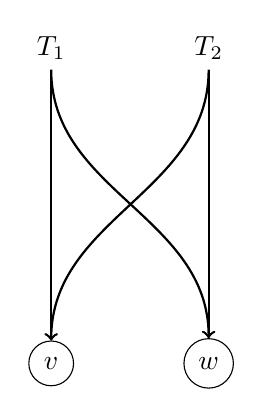
\begin{tikzpicture}
      \node (t1) at (-1,0) {$T_1$};
      \node (t2) at (1,0)  {$T_2$};
      \node (v) [draw,shape=circle] at (-1,-4) {$v$};
      \node (w) [draw,shape=circle] at (1,-4)  {$w$};

      \draw [->, thick] (t1.south) to [out=270,in=90] (v.north);
      \draw [->, thick] (t1.south) to [out=270,in=90] (w.north);
      \draw [->, thick] (t2.south) to [out=270,in=90] (v.north);
      \draw [->, thick] (t2.south) to [out=270,in=90] (w.north);
    \end{tikzpicture}
    \caption{Sequential Consistency}
  \end{subfigure}
  \begin{subfigure}{0.3\textwidth}
    \centering
    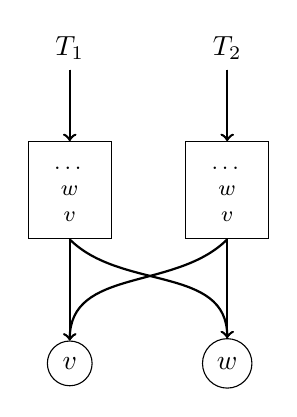
\begin{tikzpicture}
      \node (t1) at (-1,0) {$T_1$};
      \node (t2) at (1,0)  {$T_2$};
      \node (v) [draw,shape=circle] at (-1,-4) {$v$};
      \node (w) [draw,shape=circle] at (1,-4)  {$w$};

      \node (bt1) [draw] at (-1,-1.8) {\footnotesize\begin{tabular}{c} \ldots \\\midrule $w$ \\\midrule $v$ \end{tabular}};
      \node (bt2) [draw] at (1,-1.8) {\footnotesize\begin{tabular}{c} \ldots \\\midrule $w$ \\\midrule $v$ \end{tabular}};

      \draw [->, thick] (t1) to [out=270,in=90] (bt1);
      \draw [->, thick] (t1) to [out=270,in=90] (bt1);
      \draw [->, thick] (t2) to [out=270,in=90] (bt2);
      \draw [->, thick] (t2) to [out=270,in=90] (bt2);

      \draw [->, thick] (bt1.south) to [out=270,in=90] (v);
      \draw [->, thick] (bt1.south) to [out=315,in=90] (w);
      \draw [->, thick] (bt2.south) to [out=225,in=90] (v);
      \draw [->, thick] (bt2.south) to [out=270,in=90] (w);
    \end{tikzpicture}
    \caption{Total Store Order}
  \end{subfigure}
  \begin{subfigure}{0.3\textwidth}
    \centering
    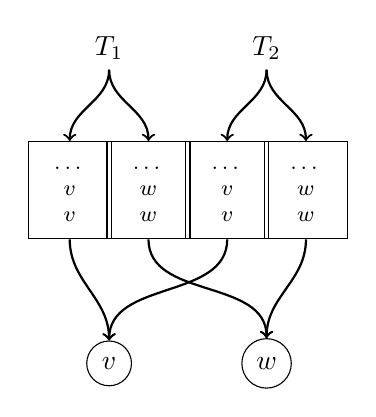
\begin{tikzpicture}
      \node (t1) at (-1,0) {$T_1$};
      \node (t2) at (1,0)  {$T_2$};
      \node (v) [draw,shape=circle] at (-1,-4) {$v$};
      \node (w) [draw,shape=circle] at (1,-4)  {$w$};

      \node (bt1v) [draw] at (-1.5,-1.8) {\footnotesize\begin{tabular}{c} \ldots \\\midrule $v$ \\\midrule $v$ \end{tabular}};
      \node (bt1w) [draw] at (-0.5,-1.8) {\footnotesize\begin{tabular}{c} \ldots \\\midrule $w$ \\\midrule $w$ \end{tabular}};
      \node (bt2v) [draw] at (0.5,-1.8) {\footnotesize\begin{tabular}{c} \ldots \\\midrule $v$ \\\midrule $v$ \end{tabular}};
      \node (bt2w) [draw] at (1.5,-1.8) {\footnotesize\begin{tabular}{c} \ldots \\\midrule $w$ \\\midrule $w$ \end{tabular}};

      \draw [->, thick] (t1) to [out=270,in=90] (bt1v);
      \draw [->, thick] (t1) to [out=270,in=90] (bt1w);
      \draw [->, thick] (t2) to [out=270,in=90] (bt2v);
      \draw [->, thick] (t2) to [out=270,in=90] (bt2w);

      \draw [->, thick] (bt1v.south) to [out=270,in=90] (v);
      \draw [->, thick] (bt1w.south) to [out=270,in=90] (w);
      \draw [->, thick] (bt2v.south) to [out=270,in=90] (v);
      \draw [->, thick] (bt2w.south) to [out=270,in=90] (w);
    \end{tikzpicture}
    \caption{Partial Store Order}
  \end{subfigure}
  \caption{Example of write buffering for two threads and two \texttt{IORef}s.}
  \label{fig:wb}
\end{figure}

We divide operations into three categories: \emph{synchronised}
operations impose a \emph{memory barrier}, committing all writes;
\emph{partially synchronised} operations commit one or more writes to
the same \verb|IORef|; and \emph{unsynchronised} operations never cause
a commit.

\paragraph{Phantom threads}
For each write buffer, we introduce a \emph{phantom thread}.  When
executed, a phantom thread commits the oldest write from its
corresponding buffer.  So when using sequentially consistency, the set
of runnable threads is exactly the set of threads created by forking
which are not blocked, but when using a relaxed memory model, this is
not the case.  This may seem like an odd approach: why create new
threads to model relaxed memory?  By using phantom threads, relaxed
memory nondeterminism becomes just another aspect of scheduling
nondeterminism.  We take this approach from \cite{zhang2015}.

\section{Operational Semantics}
\label{sec:dejafu-semantics}

Fundamental to \dejafu{} is an operational semantics for Haskell
concurrency, in the form of a step function on primitive actions.
Given the current state, which we call the context, we select a thread
to execute and either indicate a failure condition, or produce a new
context.  We also produce an execution trace for the user.  Our
semantics is similar in spirit to \cite{vollmer2017}, however we model
a much larger set of operations, and support partial store order as
well as total store order.

\newcommand{\bnfeq}{\text{::=}}
\newcommand{\bnfor}{\quad\text{|}\quad}

\begin{figure}
\centering
\[
\begin{array}{lrcl}
  \multicolumn{2}{r}{tid,~tid2} &\in&\text{Thread Identifier}\\
  \multicolumn{2}{r}{id}        &\in&\text{Heap Identifier}\\
  \multicolumn{2}{r}{a}         &\in&\text{Value}\\
  \multicolumn{2}{r}{c}         &\in&\text{Action Value}\\
  \multicolumn{2}{r}{e}         &\in&\text{Exception Value}\\
  \multicolumn{2}{r}{i,~n}      &\in&\mathbb{N}_{1}\\\\
%
  \text{Execution Context}  &\texttt{X}&\bnfeq&\langle \texttt{C},~\texttt{B},~\texttt{H},~\texttt{T} \rangle\\
  \text{Capabilities}       &\texttt{C}&\bnfeq&n\\
  \text{Buffer (TSO)}       &\texttt{B}&\bnfeq&tid \hookrightarrow [\langle id,~a \rangle]\\
  \text{Buffer (PSO)}       &\texttt{B}&\bnfeq&\langle tid,~id \rangle \hookrightarrow [a]\\
  \text{Heap}               &\texttt{H}&\bnfeq&id \hookrightarrow a\\
  \text{Thread Map}         &\texttt{T}&\bnfeq&tid \hookrightarrow \langle \texttt{K},~\texttt{E},~\texttt{M} \rangle\\\\
%
  \text{Actions}            &\texttt{K}&\bnfeq&c\\
  \text{Exception Handlers} &\texttt{E}&\bnfeq&[\lambda e \rightarrow c]\\
  \text{Exception Mask}     &\texttt{M}&\bnfeq&\text{Unmasked} \bnfor \text{Interruptible} \bnfor \text{Uninterruptible}\\
\end{array}
\]
\caption[The syntax of values and execution contexts.]{The syntax of values and execution contexts.  \Cref{lst:actionty} gives the definition of action values.}\label{fig:opsyntax}
\end{figure}

\paragraph{Syntax}
We express our semantics as transitions on execution contexts.
\Cref{fig:opsyntax} gives the syntax for these contexts.  A context
has a number of capabilities (\texttt{C}), a relaxed-memory buffer
(\texttt{B}), a heap (\texttt{H}), and a collection of threads
(\texttt{T}).  The representation of \texttt{B} depends on the memory
model: it is a finite mapping, either from thread identifiers to a
list of heap identifier and value pairs, or from thread and heap
identifier pairs to a list of values; see
\Cref{sec:dejafu-semantics-writes}.  \texttt{H} is a finite mapping
from identifiers to values.  \texttt{T} is a finite mapping from
identifiers to threads.  A thread has a next operation to perform
(\texttt{K}), a list of exception handlers (\texttt{E}), and a masking
state (\texttt{M}).

For some rules we include side-conditions or local definitions.  We
use Haskell syntax for these.

\begin{listing}
\centering
\begin{cminted}{haskell}
data Action n
  -- Basic multithreading
  = AFork String ((forall b. ConcT n b -> ConcT n b) -> Action n)
      (ThreadId -> Action n)
  | AGetNumCapabilities     (Int -> Action n)
  | ASetNumCapabilities Int        (Action n)
  | AMyTId (ThreadId -> Action n)
  | ALift  (n a)  (a -> Action n)
  | AYield             (Action n)
  | ADelay             (Action n)
  | AReturn            (Action n)
  | AStop

  -- IORefs and relaxed memory
  | forall a.   ANewIORef     String           a (ModelIORef n a -> Action n)
  | forall a.   AReadIORef    (ModelIORef n a)                (a -> Action n)
  | forall a.   AReadIORefCas (ModelIORef n a)    (ModelTicket a -> Action n)
  | forall a.   AWriteIORef   (ModelIORef n a) a                   (Action n)
  | forall a b. AModIORef     (ModelIORef n a) (a -> (a, b))  (b -> Action n)
  | forall a b. AModIORefCas  (ModelIORef n a) (a -> (a, b))  (b -> Action n)
  | forall a.   ACasIORef (ModelIORef n a) (ModelTicket a) a
      ((Bool, ModelTicket a) -> Action n)
  | ACommit ThreadId IORefId

  -- MVars
  | forall a. ANewMVar     String            (ModelMVar n a -> Action n)
  | forall a. APutMVar     (ModelMVar n a) a                  (Action n)
  | forall a. ATakeMVar    (ModelMVar n a)               (a -> Action n)
  | forall a. AReadMVar    (ModelMVar n a)               (a -> Action n)
  | forall a. ATryPutMVar  (ModelMVar n a) a          (Bool -> Action n)
  | forall a. ATryTakeMVar (ModelMVar n a)         (Maybe a -> Action n)
  | forall a. ATryReadMVar (ModelMVar n a)         (Maybe a -> Action n)

  -- Exceptions
  | forall e.   Exception e => AThrow e
  | forall e.   Exception e => AThrowTo ThreadId e (Action n)
  | forall a e. Exception e => ACatching (e -> ConcT n a) (ConcT n a)
      (a -> Action n)
  | forall a.   AMasking MaskingState
      ((forall b. ConcT n b -> ConcT n b) -> ConcT n a) (a -> Action n)
  | AResetMask   MaskingState (Action n)
  | APopCatching              (Action n)

  -- STM
  | forall a. AAtom (ModelSTM n a) (a -> Action n)
\end{cminted}
\caption{The primitive concurrency actions.}\label{lst:actionty}
\end{listing}

\paragraph{Primitive actions}
\Cref{lst:actionty} gives the primitive actions for concurrency.
Execution happens in the context of an underlying monad, the \verb|n|
parameter to the \verb|Action| type.  This monad is usually \verb|IO|,
but can be any \verb|MonadConc|.  In these semantics we only use this
monad for the \verb|ALift| action.  \dejafu{} communicates the result
of the computation back to the caller by inserting an \verb|ALift|
action which writes the result of the main thread to a mutable
reference just before termination.

Our implementation of model execution is more similar to cooperative
multitasking than pre-emptive multitasking: if evaluating a primitive
action fails to terminate, the entire computation locks up.

\paragraph{Simplifications and omissions}
The semantic rules we present are for the small-step behaviour.  They
are tied together by a scheduling loop which we do not present here.
This scheduling loop picks a thread to step, steps it, and continues
until every thread is blocked or the main thread terminates.

For presentation purposes, we omit some of the complexities of the
implementation.  We omit building the execution trace, and we omit the
definition of helper functions, but explain them when first used.
Furthermore, while we present the heap here as a heterogeneous map, in
practice we implement it using real mutable references.

\newcommand{\semfullthread}[3]{\langle\texttt{#1}, \texttt{#2}, \texttt{#3}\rangle}
\newcommand{\semthread}[1]{\semfullthread{#1}{E}{M}}

\newcommand{\semlfullrule}[4]{\langle\texttt{C}_{#1}, \texttt{B}_{#2}, \texttt{H}_{#3}, \texttt{T}_{\left[\texttt{tid} \mapsto \semthread{#4}\right]}\rangle}
\newcommand{\semlheaprule}[2]{\semlfullrule{}{}{[\texttt{id} \mapsto \texttt{#2}]}{#1}}
\newcommand{\semlrule}[1]{\semlfullrule{}{}{}{#1}}

\subsection{Basic Concurrency}

\begin{figure}
\centering
\begin{tabular}{r@{\hspace{0.5em}}l}
$\langle\texttt{C}, \texttt{B}, \texttt{H}, \texttt{T}_{\left[\texttt{tid} \mapsto \semfullthread{AFork \_ act c}{E}{m0}\right]}\rangle\rightarrow$&
$\langle\texttt{C}, \texttt{B}, \texttt{H}, \texttt{T}_{[\texttt{tid} \mapsto \semfullthread{c tid2}{E}{m0};~\texttt{tid2} \mapsto \texttt{new}]}\rangle$\\
\multicolumn{2}{l}{where \texttt{tid2} is not in the domain of \texttt{T}}\\
\multicolumn{2}{l}{\hphantom{where }$\texttt{reset m'} = \texttt{\textbackslash k -> AResetMask m' k}$}\\
\multicolumn{2}{l}{\hphantom{where }$\texttt{umask mb} = \texttt{reset Unmasked >> mb >> \textbackslash b -> reset m0 >> pure b}$}\\
\multicolumn{2}{l}{\hphantom{where }$\texttt{new} = \langle\texttt{act umask}, \texttt{[]}, \texttt{m0}\rangle$}\\
& \\
$\semlrule{AGetNumCapabilities c}\rightarrow$&
$\langle\texttt{C}, \texttt{B}, \texttt{H}, \texttt{T}_{[\texttt{tid} \mapsto \semthread{c C}]}\rangle$\\
$\semlrule{ASetNumCapabilities i c}\rightarrow$&
$\langle\texttt{i}, \texttt{B}, \texttt{H}, \texttt{T}_{[\texttt{tid} \mapsto \semthread{c}]}\rangle$\\
$\semlrule{AMyTId c}\rightarrow$&
$\langle\texttt{C}, \texttt{B}, \texttt{H}, \texttt{T}_{[\texttt{tid} \mapsto \semthread{c tid}]}\rangle$\\
$\semlrule{AYield c}\rightarrow$&
$\langle\texttt{C}, \texttt{B}, \texttt{H}, \texttt{T}_{[\texttt{tid} \mapsto \semthread{c}]}\rangle$\\
$\semlrule{ADelay c}\rightarrow$&
$\langle\texttt{C}, \texttt{B}, \texttt{H}, \texttt{T}_{[\texttt{tid} \mapsto \semthread{c}]}\rangle$\\
$\semlrule{AReturn c}\rightarrow$&
$\langle\texttt{C}, \texttt{B}, \texttt{H}, \texttt{T}_{[\texttt{tid} \mapsto \semthread{c}]}\rangle$\\
$\semlrule{ALift na c}\rightarrow$&
$\langle\texttt{C}, \texttt{B}, \texttt{H}, \texttt{T}_{[\texttt{tid} \mapsto \semthread{na >>= c}]}\rangle$\\
$\semlrule{AStop}\rightarrow$&
$\langle\texttt{C}, \texttt{B}, \texttt{H}, \texttt{T}_{[\texttt{tid} \mapsto \varnothing]}\rangle$
\end{tabular}
\caption{Transition semantics of basic multithreading actions.}\label{fig:sem_multithreading}
\end{figure}

\Cref{fig:sem_multithreading} shows the semantics for the basic
multithreading operations.  These rules do not involve memory, so they
leave the relaxed-memory buffer and heap untouched.  We write
$\texttt{M}_{[\texttt{k} \mapsto \texttt{v}]}$ to denote a new map
which maps the key \texttt{k} to the value \texttt{v}.

Rather than have one primitive action for each of the \verb|fork|-like
functions, we only provide \verb|AFork|, which implements
\verb|forkWithUnmask| for named threads, and implement the others in
terms of this.  We do not model which capability a thread is executing
on, so we do not also need an ``\verb|AForkOn|'' action.

The \verb|ALift| and \verb|AStop| actions are a little unlike the
others.  \verb|ALift| causes a Haskell-level effect to occur by
executing some action in the underlying monad.  \verb|AStop| has no
continuation, we use $\texttt{T}_{[\texttt{tid}\mapsto\varnothing]}$
to mean that the thread is deleted.

\paragraph{\texttt{IORef} operations}
\Cref{fig:sem_ioref} shows the semantics for the \verb|IORef|
operations.  We represent a \verb|IORef| as reference to a pair of a
number of commits and a latest value.  We present the rules for
writing to and committing to an \verb|IORef|, which depends on the
memory model, in \Cref{sec:dejafu-semantics-writes}

We use $\texttt{H} \oplus \texttt{B}$ to mean a new heap with all
buffered writes committed, nondeterministically, in some order
permitted by the memory model.  This is a memory barrier.  We use
$\texttt{H} \oplus \texttt{B}_{[\texttt{tid}]}$ to mean that only the
buffered writes from thread \verb|tid| are committed.  Under
sequential consistency there are no buffered writes, so
$\texttt{H} \oplus \texttt{\_} = \texttt{H}$.

\paragraph{\texttt{MVar} operations}
\Cref{fig:sem_mvar} shows the semantics for the \verb|MVar|
operations.  We represent an \verb|MVar| as a reference to a
\verb|Maybe| value.  These operations enforce a memory barrier, and
some may cause the thread to block.  An action can enforce a memory
barrier even if it blocks.  We model blocking by not changing the
continuation for the chosen thread.

\paragraph{Exceptions and masking}
\Cref{fig:sem_exc} shows the semantics for the exception and masking
operations.  The \verb|raise| function pops from a stack of exception
handlers until it finds a handler for the given exception.  The
\verb|interruptible| function checks if the given thread can be
interrupted with an exception.  A thread can be interrupted if its
masking state is ``unmasked'', or if its masking state is
``interruptible'' and it is blocked.

The \verb|AMasking| action is similar to \verb|AFork|: it runs an
action after passing an argument to change the masking state.
However, unlike \verb|AFork|, \verb|AMasking| runs the action in the
current thread rather than creating a new one.

\begin{figure}
\centering
\begin{tabular}{r@{\hspace{0.5em}}l}
$\semlrule{ANewIORef \_ a c}\rightarrow$&
$\langle\texttt{C}, \texttt{B}, \texttt{H}_{[\texttt{id} \mapsto \texttt{(0, a)}]}, \texttt{T}_{[\texttt{tid} \mapsto \semthread{c id}]}\rangle$ \\
\multicolumn{2}{l}{where \texttt{id} is not in the domain of \texttt{H}}\\
& \\
$\semlrule{AReadIORef id c}\rightarrow$&
$\langle\texttt{C}, \texttt{B}, \texttt{H}, \texttt{T}_{[\texttt{tid} \mapsto \semthread{c x}]}\rangle$ \\
\multicolumn{2}{l}{where $\texttt{(\_, x)} = (\texttt{H} \oplus \texttt{B}_{[\texttt{tid}]})_{[\texttt{id}]}$}\\
& \\
$\semlrule{AReadIORefCAS id c}\rightarrow$&
$\langle\texttt{C}, \texttt{B}, \texttt{H}, \texttt{T}_{[\texttt{tid} \mapsto \semthread{c (Ticket id n x)}]}\rangle$ \\
\multicolumn{2}{l}{where $\texttt{(n, x)} = (\texttt{H} \oplus \texttt{B}_{[\texttt{tid}]})_{[\texttt{id}]}$}\\
& \\
$\semlrule{AModIORef id f c}\rightarrow$&\\
\multicolumn{2}{r}{$\langle\texttt{C}, \varnothing, (\texttt{H} \oplus \texttt{B})_{[\texttt{id} \mapsto \texttt{(n+1, f a)}]}, \texttt{T}_{[\texttt{tid} \mapsto \semthread{c}]}\rangle$}\\
\multicolumn{2}{l}{where $\texttt{(n, a)} = \texttt{H} \oplus \texttt{B}_{[\texttt{tid}]}$}\\
& \\
$\semlrule{AModIORefCAS id f c}\rightarrow$&\\
\multicolumn{2}{r}{$\langle\texttt{C}, \varnothing, (\texttt{H} \oplus \texttt{B})_{[\texttt{id} \mapsto \texttt{(n+1, f a)}]}, \texttt{T}_{[\texttt{tid} \mapsto \semthread{c}]}\rangle$}\\
\multicolumn{2}{l}{where $\texttt{(n, a)} = (\texttt{H} \oplus \texttt{B})_{[\texttt{id}]}$}\\
& \\
\multicolumn{2}{l}{$\semlrule{ACasIORef id (Ticket id n \_) a} \rightarrow$}\\
\multicolumn{2}{r}{$\langle\texttt{C}, \varnothing, (\texttt{H} \oplus \texttt{B})_{[\texttt{id} \mapsto \texttt{(n+1, a)}]}, \texttt{T}_{[\texttt{tid} \mapsto \semthread{c (True, Ticket id (n+1) a)}]}\rangle$}\\
\multicolumn{2}{l}{if $\texttt{n} = \texttt{n0}$}\\
\multicolumn{2}{l}{where $\texttt{(n0, \_)} = (\texttt{H} \oplus \texttt{B})_{[\texttt{id}]}$}\\
& \\
\multicolumn{2}{l}{$\semlrule{ACasIORef id (Ticket id n \_) \_} \rightarrow$}\\
\multicolumn{2}{r}{$\langle\texttt{C}, \varnothing, \texttt{H} \oplus \texttt{B}, \texttt{T}_{[\texttt{tid} \mapsto \semthread{c (False, Ticket id n0 a0)}]}\rangle$}\\
\multicolumn{2}{l}{if $\texttt{n} \neq \texttt{n0}$}\\
\multicolumn{2}{l}{where $\texttt{(n0, a0)} = (\texttt{H} \oplus \texttt{B})_{[\texttt{id}]}$}\\
&
\end{tabular}
\caption{Transition semantics of \texttt{IORef} actions.}\label{fig:sem_ioref}
\end{figure}

\begin{figure}
\centering
\begin{tabular}{r@{\hspace{0.5em}}l}
\multicolumn{2}{r}{$\semlrule{ANewMVar \_ c} \rightarrow \langle\texttt{C}, \texttt{B}, \texttt{H}_{[\texttt{id} \mapsto \texttt{Nothing}]}, \texttt{T}_{[\texttt{tid} \mapsto \semthread{c id}]}\rangle$}\\
\multicolumn{2}{l}{where \texttt{id} is not in the domain of \texttt{H}}\\
& \\
$\semlheaprule{APutMVar id \_ \_}{Just \_}$\hfill$\rightarrow$&
$\langle\texttt{C}, \varnothing, \texttt{H} \oplus \texttt{B}, \texttt{T}\rangle$\\
& \\
$\semlheaprule{APutMVar id a c}{Nothing}$\hfill$\rightarrow$&\\
\multicolumn{2}{r}{$\langle\texttt{C}, \varnothing, \texttt{H}_{[\texttt{id} \mapsto \texttt{Just a}]} \oplus \texttt{B}, \texttt{T}_{[\texttt{tid} \mapsto \semthread{c}]}\rangle$}\\
& \\
$\semlheaprule{ATakeMVar id c}{Just x}$\hfill$\rightarrow$&\\
\multicolumn{2}{r}{$\langle\texttt{C}, \varnothing, \texttt{H}_{[\texttt{id} \mapsto \texttt{Nothing}]} \oplus \texttt{B}, \texttt{T}_{[\texttt{tid} \mapsto \semthread{c x}]}\rangle$}\\
& \\
$\semlheaprule{ATakeMVar id \_ \_}{Nothing}$\hfill$\rightarrow$&
$\langle\texttt{C}, \varnothing, \texttt{H} \oplus \texttt{B}, \texttt{T}\rangle$\\
& \\
$\semlheaprule{AReadMVar id c}{Just x}\rightarrow$&
$\langle\texttt{C}, \varnothing, \texttt{H} \oplus \texttt{B}, \texttt{T}_{[\texttt{tid} \mapsto \semthread{c x}]}\rangle$\\
& \\
$\semlheaprule{AReadMVar id \_ \_}{Nothing}$\hfill$\rightarrow$&
$\langle\texttt{C}, \varnothing, \texttt{H} \oplus \texttt{B}, \texttt{T}\rangle$\\
& \\
$\semlheaprule{ATryPutMVar id c}{Just \_}$\hfill$\rightarrow$&\\
\multicolumn{2}{r}{$\langle\texttt{C}, \varnothing, \texttt{H} \oplus \texttt{B}, \texttt{T}_{[\texttt{tid} \mapsto \semthread{c False}]}\rangle$}\\
& \\
$\semlheaprule{ATryPutMVar id a c}{Nothing}$\hfill$\rightarrow$&\\
\multicolumn{2}{r}{$\langle\texttt{C}, \varnothing, \texttt{H}_{[\texttt{id} \mapsto \texttt{Just a}]} \oplus \texttt{B}, \texttt{T}_{[\texttt{tid} \mapsto \semthread{c True}]}\rangle$}\\
& \\
$\semlheaprule{ATryTakeMVar id c}{Just x}$\hfill$\rightarrow$&\\
\multicolumn{2}{r}{$\langle\texttt{C}, \varnothing, \texttt{H}_{[\texttt{id} \mapsto \texttt{Nothing}]} \oplus \texttt{B}, \texttt{T}_{[\texttt{tid} \mapsto \semthread{c (Just x)}]}\rangle$}\\
& \\
$\semlheaprule{ATryTakeMVar id c}{Nothing}$\hfill$\rightarrow$&\\
\multicolumn{2}{r}{$\langle\texttt{C}, \varnothing, \texttt{H} \oplus \texttt{B}, \texttt{T}_{[\texttt{tid} \mapsto \semthread{c Nothing}]}\rangle$}\\
& \\
$\semlheaprule{ATryReadMVar id c}{x}\rightarrow$&
$\langle\texttt{C}, \varnothing, \texttt{H} \oplus \texttt{B}, \texttt{T}_{[\texttt{tid} \mapsto \semthread{c x}]}\rangle$
\end{tabular}
\caption{Transition semantics of \texttt{MVar} actions.}\label{fig:sem_mvar}
\end{figure}

\begin{figure}
\centering
\begin{tabular}{r@{\hspace{0.5em}}l}
$\langle\texttt{C}, \texttt{B}, \texttt{H}, \texttt{T}_{\left[\texttt{tid} \mapsto \semfullthread{AThrow e}{hs}{M}\right]}\rangle\rightarrow$&
$\langle\texttt{C}, \texttt{B}, \texttt{H}, \texttt{T}_{[\texttt{tid} \mapsto \varnothing]}\rangle$ \\
\multicolumn{2}{l}{if $\texttt{null (raise hs e)}$}\\
& \\
$\langle\texttt{C}, \texttt{B}, \texttt{H}, \texttt{T}_{\left[\texttt{tid} \mapsto \semfullthread{AThrow e}{hs}{M}\right]}\rangle\rightarrow$&
$\langle\texttt{C}, \texttt{B}, \texttt{H}, \texttt{T}_{[\texttt{tid} \mapsto \semfullthread{h e}{hs}{M}]}\rangle$ \\
\multicolumn{2}{l}{if \texttt{not (null (raise hs e))}}\\
\multicolumn{2}{l}{where \texttt{(h:hs)} = \texttt{raise hs e}}\\
& \\
$\semlrule{AThrowTo id e c}\rightarrow$\\
\multicolumn{2}{r}{$\langle\texttt{C}, \varnothing, \texttt{H} \oplus \texttt{B}, \texttt{T}_{[\texttt{tid} \mapsto \semthread{c};~\texttt{id} \mapsto \semfullthread{AThrow e}{E'}{M'}]}\rangle$}\\
\multicolumn{2}{l}{if \texttt{interruptible id}}\\
\multicolumn{2}{l}{where $\langle\texttt{\_}, \texttt{E'}, \texttt{M'}\rangle = \texttt{T}_{[\texttt{id}]}$}\\
& \\
$\semlrule{AThrowTo id \_ \_}\rightarrow$&
$\langle\texttt{C}, \varnothing, \texttt{H} \oplus \texttt{B}, \texttt{T}\rangle$\\
\multicolumn{2}{l}{if \texttt{not (interruptible id)}}\\
& \\
$\langle\texttt{C}, \texttt{B}, \texttt{H}, \texttt{T}_{\left[\texttt{tid} \mapsto \semfullthread{ACatching i inner c}{hs}{M}\right]}\rangle\rightarrow$&\\
\multicolumn{2}{r}{$\langle\texttt{C}, \texttt{B}, \texttt{H}, \texttt{T}_{[\texttt{tid} \mapsto \semfullthread{inner (APopCatching . c)}{h:hs}{M}]}\rangle$} \\
& \\
$\langle\texttt{C}, \texttt{B}, \texttt{H}, \texttt{T}_{\left[\texttt{tid} \mapsto \semfullthread{APopCatching c}{\_:hs}{M}\right]}\rangle\rightarrow$&
$\langle\texttt{C}, \texttt{B}, \texttt{H}, \texttt{T}_{[\texttt{tid} \mapsto \semfullthread{c}{hs}{M}]\rangle}$ \\
& \\
$\langle\texttt{C}, \texttt{B}, \texttt{H}, \texttt{T}_{\left[\texttt{tid} \mapsto \semfullthread{AMasking m act c}{E}{m0}\right]}\rangle\rightarrow$&\\
\multicolumn{2}{r}{$\langle\texttt{C}, \texttt{B}, \texttt{H}, \texttt{T}_{[\texttt{tid} \mapsto \semfullthread{act umask (AResetMask m0 . c)}{E}{m}]}\rangle$} \\
& \\
\multicolumn{2}{l}{where $\texttt{m0} = \texttt{T}_{[\texttt{tid}.\texttt{M}]}$}\\
\multicolumn{2}{l}{\hphantom{where }$\texttt{reset m'} = \texttt{\textbackslash k -> AResetMask m' (k)}$}\\
\multicolumn{2}{l}{\hphantom{where }$\texttt{umask mb} = \texttt{reset m0 >> mb >> \textbackslash b -> reset m >> pure b}$}\\
& \\
$\semlrule{AResetMask m c}\rightarrow$&
$\langle\texttt{C}, \texttt{B}, \texttt{H}, \texttt{T}_{[\texttt{tid} \mapsto \semfullthread{c}{E}{m}]}\rangle$
\end{tabular}
\caption{Transition semantics of exception actions.}\label{fig:sem_exc}
\end{figure}

\subsection{The Memory Model}
\label{sec:dejafu-semantics-writes}

To avoid giving all of our semantic rules which read from memory three
times, we have used the $\oplus$ operator, to denote synchronising any
buffered writes to the global memory in a nondeterministic fashion.
The behaviour of this operator depends on the memory model used.

\begin{itemize}
\item Under sequential consistency, there are no buffered writes, so
  $\texttt{H} \oplus \texttt{\_} = \texttt{H}$.
\item Under total store order, we give each thread a buffer, so
  \verb|B| is a map from thread identifiers to sequences of writes.
  Here $\texttt{H} \oplus \texttt{B}$ selects a thread with buffered
  writes nondeterministically, and pops and performs the oldest write
  from its buffer.  This process is repeated until there are no
  remaining buffered writes.
\item Under partial store order, there is a buffer for each (thread,
  \verb|IORef|) pair, but the process is otherwise the same as for
  TSO.
\end{itemize}

\paragraph{Writing to an \texttt{IORef}}
\Cref{fig:sem_ioref_relaxed_w} gives the semantic rules for writing to
an \verb|IORef|.  There is one rule for each memory model,
corresponding to the buffering strategy used.  Under sequential
consistency, the write goes straight to the heap; under TSO, the write
is appended to the buffer for the chosen thread; and under PSO the
write is appended to the buffer for the chosen (thread, \verb|IORef|)
pair.

\paragraph{Committing buffered writes}
\Cref{fig:sem_ioref_relaxed_c} gives the semantic rules for committing
buffered \verb|IORef| writes.  There is no rule for sequential
consistency, as there are no buffered writes in that case.  Another
way to think of the $\oplus$ operator is that it performs all possible
commit actions.

\begin{figure}
\centering
\begin{tabular}{r@{\hspace{0.5em}}l}
\multicolumn{2}{c}{$\semlrule{AWriteIORef id a c}\rightarrow\langle\texttt{C}, \texttt{B}, \texttt{H}_{[\texttt{id} \mapsto \texttt{(0, a)}]}, \texttt{T}_{[\texttt{tid} \mapsto \semthread{c}]}\rangle$}\\
\multicolumn{2}{l}{if using sequential consistency}\\
& \\
$\semlfullrule{}{[\texttt{tid} \mapsto \texttt{buf}]}{}{AWriteIORef id a c}\rightarrow$&\\
\multicolumn{2}{r}{$\langle\texttt{C}, \texttt{B}_{[\texttt{tid} \mapsto \texttt{(buf ++ (id, a))}]}, \texttt{H}, \texttt{T}_{[\texttt{tid} \mapsto \semthread{c}]}\rangle$}\\
\multicolumn{2}{l}{if using total store order}\\
& \\
$\semlfullrule{}{[\texttt{(tid, id)} \mapsto \texttt{buf}]}{}{AWriteIORef id a c}\rightarrow$&\\
\multicolumn{2}{r}{$\langle\texttt{C}, \texttt{B}_{[\texttt{(tid, id)} \mapsto \texttt{(buf ++ a)}]}, \texttt{H}, \texttt{T}_{[\texttt{tid} \mapsto \semthread{c}]}\rangle$}\\
\multicolumn{2}{l}{if using partial store order}
\end{tabular}
\caption{Transition semantics of writing to \texttt{IORef}s.}\label{fig:sem_ioref_relaxed_w}
\end{figure}

\begin{figure}
\centering
\begin{tabular}{r@{\hspace{0.5em}}l}
$\langle\texttt{C}, \texttt{B}_{[\texttt{tid} \mapsto \texttt{((id, a):buf)}]}, \texttt{H}_{[\texttt{id} \mapsto \texttt{(n, \_)}]}, \texttt{T}\rangle \rightarrow$&
$\langle\texttt{C}, \texttt{B}_{[\texttt{tid} \mapsto \texttt{buf}]}, \texttt{H}_{[\texttt{id} \mapsto \texttt{(n+1, a)}]}, \texttt{T}\rangle$ \\
\multicolumn{2}{l}{if using total store order}\\
$\langle\texttt{C}, \texttt{B}_{[\texttt{(tid, id)} \mapsto \texttt{(a:buf)}]}, \texttt{H}_{[\texttt{id} \mapsto \texttt{(n, \_)}]}, \texttt{T}\rangle \rightarrow$&
$\langle\texttt{C}, \texttt{B}_{[\texttt{(tid, id)} \mapsto \texttt{buf}]}, \texttt{H}_{[\texttt{id} \mapsto \texttt{(n+1, a)}]}, \texttt{T}\rangle$ \\
\multicolumn{2}{l}{if using partial store order}
\end{tabular}
\caption{Transition semantics of committing \texttt{IORef} writes.}\label{fig:sem_ioref_relaxed_c}
\end{figure}

\subsection{Software Transactional Memory}

Here we only give the semantics of the \verb|AAtom| action, a full
operational semantics of STM is given in \cite{harris2005}.  The STM
semantics are small-step reductions of the form
$M; \Theta, \Delta \Rightarrow N; \Theta', \Delta'$, where $M$ and $N$
are Haskell expressions, $\Theta$ is the heap, and $\Delta$ is the set
of \verb|TVar| variables which have been accessed.  We use
$\xRightarrow{*}$ to denote a sequence of multiple small-step
reductions.

\begin{figure}[h]
\centering
\begin{prooftree}
\AxiomC{$\texttt{stm};~\texttt{H} \oplus \texttt{B}, \varnothing \xRightarrow{*} \texttt{return x};~\texttt{H'}, \texttt{\_}$}
\UnaryInfC{$\semlrule{AAtom stm c} \rightarrow \langle\texttt{C}, \varnothing, \texttt{H'}, \texttt{T}_{[\texttt{tid} \mapsto \semthread{c x}]}\rangle$}
\end{prooftree}

\begin{prooftree}
\AxiomC{$\texttt{stm};~\texttt{H} \oplus \texttt{B}, \varnothing \xRightarrow{*} \texttt{throw x};~\texttt{H'}, \texttt{\_}$}
\UnaryInfC{$\semlrule{AAtom stm \_} \rightarrow \langle\texttt{C}, \varnothing, \texttt{H'}, \texttt{T}_{[\texttt{tid} \mapsto \semthread{AThrow x}]}\rangle$}
\end{prooftree}

\begin{prooftree}
\AxiomC{$\texttt{stm};~\texttt{H} \oplus \texttt{B}, \varnothing \xRightarrow{*} \texttt{retry};~\texttt{\_}, \texttt{\_}$}
\UnaryInfC{$\semlrule{AAtom stm \_} \rightarrow \langle\texttt{C}, \varnothing, \texttt{H} \oplus \texttt{B}, \texttt{T}\rangle$}
\end{prooftree}
\caption{Transition semantics for \texttt{AAtom}.}\label{fig:sem_aatom}
\end{figure}

\Cref{fig:sem_aatom} gives the semantics of executing transactions.
Executing an STM transaction enforces a memory barrier, and writes
inside the transaction are synchronised.  If the transaction reduces
to a \verb|throw| expression, the exception is re-thrown in the
thread.  As in the \verb|MVar| and exception semantics, a transaction
which blocks still imposes a memory barrier.

\FloatBarrier
\section{Testing Concurrent Programs}
\label{sec:dejafu-testing}

\dejafu{} uses a combination of DPOR and schedule bounding to test
programs by default.  Controlled random scheduling using a fixed
number of executions is also available.  The testing algorithm to use,
and its configuration, is controlled with the \verb|Settings|
value~\sref{dejafu-whatis}.

\begin{figure}
  \centering
  \footnotesize
  \begin{tabular}{R{4cm}@{\hspace{0.5em}}L{8cm}}
    \texttt{atomicModifyIORef r \_} $\dependent$& \texttt{x}
      \hfill if \texttt{x} uses \texttt{r} \\
    \texttt{atomically x} $\dependent$& \texttt{atomically y}
      \hfill if \texttt{x} writes to a \texttt{TVar} which \texttt{y} accesses \\
    \texttt{casIORef r \_} $\dependent$& \texttt{x}
      \hfill if \texttt{x} uses \texttt{r} \\
    \texttt{commit \_} $\dependent$& \texttt{b}
      \hfill if \texttt{b} enforces a memory barrier \\
    \texttt{commit r} $\dependent$& \texttt{writeIORef r}
      \hfill if \texttt{r} has no buffered writes \\
    \texttt{commit r} $\dependent$& \texttt{x}
      \hfill if \texttt{x} uses \texttt{r} and is not a \texttt{writeIORef r} \\
    \texttt{crefRead r} $\dependent$& \texttt{b}
      \hfill if \texttt{b} enforces a memory barrier and \texttt{r} has buffered writes \\
    \texttt{crefRead r} $\dependent$& \texttt{x}
      \hfill if \texttt{x} uses \texttt{r} and is not a \texttt{crefRead r} \\
    \texttt{liftIO \_} $\dependent$& \texttt{liftIO \_} \\
    \texttt{modifyIORefCAS r \_} $\dependent$& \texttt{x}
      \hfill if \texttt{x} uses \texttt{r} \\
    \texttt{mvarRead v} $\dependent$& \texttt{mvarRead v}
      \hfill if \texttt{v} is full \\
    \texttt{mvarRead v} $\dependent$& \texttt{mvarWrite v} \\
    \texttt{mvarWrite v} $\dependent$& \texttt{mvarWrite v}
      \hfill if \texttt{v} is empty \\
    \texttt{setNumCapabilities \_} $\dependent$& \texttt{getNumCapabilities} \\
    \texttt{setNumCapabilities \_} $\dependent$& \texttt{setNumCapabilities \_} \\
    \texttt{throwTo tgt} $\dependent$& \texttt{x}
      \hfill if \texttt{x} is on thread \texttt{tgt} and can be interrupted \\
    \texttt{writeIORef r \_} $\dependent$& \texttt{x}
      \hfill if \texttt{x} uses \texttt{r} and is not a \texttt{commit r} \\
    \texttt{x} $\dependent$& \texttt{y}
      \hfill if \texttt{y} $\dependent$ \texttt{x}
  \end{tabular}
  \caption[The \dejafu{} dependency relation.]{The \dejafu{} dependency relation.  A \texttt{commit} commits one buffered write to a \texttt{IORef}.  A \texttt{crefRead} is a \texttt{readIORef} or a \texttt{readForCAS}.  An \texttt{mvarWrite} is a \texttt{putMVar} or a \texttt{tryPutMVar}.  An \texttt{mvarRead} is a \texttt{takeMVar}, \texttt{tryTakeMVar}, \texttt{readMVar}, or \texttt{tryReadMVar}.}\label{fig:deprel}
\end{figure}

\paragraph{Dependency relation}
DPOR uses a dependency relation between pairs of actions.  Two actions
are dependent if the order in which they are performed matters.  This
relation may have false positives, but cannot have false negatives.
False positives lead to exploring redundant executions, false
negatives lead to missing distinct ones.

For ease of explanation, DPOR algorithms in the literature are
presented for small languages.  A paper will typically start with a
sentence like ``we assume a core concurrent language of reads and
writes to shared variables, and locks.''  For example, in
\cite{coons2013} two actions are said to be dependent if they are
actions of the same thread, or they are both actions on the same
shared variable and at least one is a write.  The Haskell concurrency
API is richer than this, and the implicit dependencies between actions
(such as which actions impose a memory barrier) are not documented.

\Cref{fig:deprel} shows the dependency relation we use in \dejafu{}.
We use a conditional dependency relation \parencite{godefroid1993}.
Whether two actions are dependent depends on an approximation of the
current state: we record which \verb|IORef|s have buffered writes,
whether each \verb|MVar| is full or empty, and what the masking state
of every thread is.  A conditional dependency relation allows more
precise decisions.

\begin{figure}
  \centering
  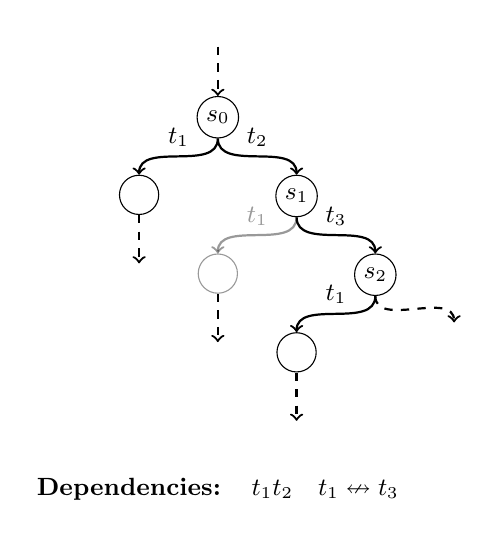
\begin{tikzpicture}[ball/.style = {circle, draw, align=center, anchor=north, inner sep=0, text width=0.5cm}]
    \node[ball]              (A) at (0,0)   {\small $s_0$};
    \node[ball]              (B) at (-1,-1) {};
    \node[ball]              (C) at (1,-1)  {\small $s_1$};
    \node[ball, opacity=0.4] (D) at (0,-2)  {};
    \node[ball]              (E) at (2,-2)  {\small $s_2$};
    \node[ball]              (F) at (1,-3)  {};

    \node (init) at (0,0.75)   {};
    \node (end1) at (-1,-2.25) {};
    \node (end2) at (0,-3.25)  {};
    \node (end3) at (3,-3)     {};
    \node (end4) at (1,-4.25)  {};
    \draw[->, thick, draw, dashed] (init.south) to [out=270,in=90] (A.north);
    \draw[->, thick, draw, dashed] (B.south) to [out=270,in=90] (end1.north);
    \draw[->, thick, draw, dashed] (D.south) to [out=270,in=90] (end2.north);
    \draw[->, thick, draw, dashed] (E.south) to [out=270,in=90] (end3.north);
    \draw[->, thick, draw, dashed] (F.south) to [out=270,in=90] (end4.north);

    \draw[->, thick, draw]              (A.south) to [out=270,in=90] node[midway,above] {\small $t_1$} (B.north);
    \draw[->, thick, draw]              (A.south) to [out=270,in=90] node[midway,above] {\small $t_2$} (C.north);
    \draw[->, thick, draw, opacity=0.4] (C.south) to [out=270,in=90] node[midway,above] {\small $t_1$} (D.north);
    \draw[->, thick, draw]              (C.south) to [out=270,in=90] node[midway,above] {\small $t_3$} (E.north);
    \draw[->, thick, draw]              (E.south) to [out=270,in=90] node[midway,above] {\small $t_1$} (F.north);

    \node (note) at (0,-5) {
      \small \textbf{Dependencies:} \hspace{0.1cm} $t_1 \independent t_2$ \hspace{0.1cm} $t_1 \dependent t_3$
    };
  \end{tikzpicture}
  \caption[The sleep set optimisation.]{The sleep set optimisation.  Transition $t_1$ may be pruned in state $s_1$ but not in state $s_2$.  The transition has been explored from state $s_0$ and there is no dependent transition between states $s_0$ and $s_1$, but there is between states $s_0$ and $s_2$.  Adapted from \cite{coons2013}.}\label{fig:sleep}
\end{figure}

\paragraph{Sleep sets}
The sleep set optimisation \parencite{godefroid1996} is a complementary
approach to DPOR which we use to further reduce schedules explored.
The intuition is as follows: if we are in a state $s_{0}$ and have a
choice of two scheduling decisions, $t_{1}$ and $t_{2}$, after trying
out $t_{1}$ there is no point in making the sequence of decisions
$t_{2}t_{1}$ from $s_{0}$, unless $t_{1} \dependent t_{2}$.  All
states reachable from $t_{1}$ have already been explored, so the only
way a new state could arise is if $t_{1}$ had a different effect,
which will only be the case if a dependent transition has been taken.
\Cref{fig:sleep} shows this graphically.

Formally, we augment each state $s$ with a \emph{sleep set},
containing transitions enabled in $s$ but which we will not make.  The
initial state has an empty sleep set.  Let $T$ be the transitions that
have been selected to be explored from $s$.  We proceed as follows:
take a transition $t_{1}$ out of $T$.  The sleep set associated with
the state reached after executing $t_{1}$ from $s$ is the sleep set
associated with $s$, minus all transitions that are dependent with
$t_{1}$.  Let $t_{2}$ be a second transition taken out of $T$.  The
sleep set associated with the state reached after executing $t_{2}$
from $s$ is the sleep set associated with $s$ augmented with $t_{1}$,
minus all transitions that are dependent with $t_{2}$.  We continue
until all transitions in $T$ have been explored, at each step adding
the previously taken transitions to the sleep set of the new state,
and removing the dependent transitions.

\paragraph{Schedule bounding}
\dejafu{} supports pre-emption bounding \parencite{musuvathi2007};
fair bounding \parencite{musuvathi2008}; and depth, or length,
bounding \parencite{russell2002}.  We use a variant of the bounded
partial-order reduction algorithm~(BPOR) \parencite{coons2013},
augmented with support for relaxed memory \parencite{zhang2015}, as
our core testing algorithm.  All three bounds are enabled by default.

\paragraph{Daemon threads}
A daemon thread is a thread which is automatically killed after the
last non-daemon thread terminates.  In Haskell, every thread other
than the main thread is a daemon thread, so as soon as the main thread
terminates the whole program terminates.  This is a problem for DPOR,
as it makes the last action of the execution dependent with everything
else in the program!

\begin{listing}
\centering
\begin{cminted}{haskell}
main = do
  v <- newEmptyMVar
  fork (myThreadId >> putMVar v "hello world")
  tryReadMVar v
\end{cminted}
\caption{A program with a race condition.}\label{lst:daemon1}
\end{listing}

\Cref{lst:daemon1} gives a small concurrent program with two possible
results: \verb|Nothing|, and \verb|Just "hello world"|.  If the
scheduler favours the main thread we only see the \verb|Nothing| case,
as there is no dependency between \verb|myThreadId| and
\verb|tryReadMVar|.  Introducing a dependency between the last action
of the execution (the \verb|tryReadMVar v| in this case) and
everything else solves this problem.

\begin{listing}
\centering
\begin{cminted}{haskell}
main = do
  v <- newEmptyMVar
  fork (myThreadId >> myThreadId >> putMVar v "hello world")
  tryReadMVar v
\end{cminted}
\caption{Another program with a race condition.}\label{lst:daemon2}
\end{listing}

However, these new dependencies also present a difficulty.  In
\Cref{lst:daemon2}, the forked thread now performs \verb|myThreadId|
twice.  If the \verb|tryReadMVar| happens after the second of these,
we get the same result as if it happens after the first.  Normally,
DPOR would recognise this and prune the redundant decision, as
\verb|myThreadId| and \verb|tryReadMVar| are independent.  However, by
introducing a dependency between the final action and everything else,
we have said that it is \emph{not} redundant!  In general, introducing
a dependency like this will lead to many redundant executions which we
would otherwise avoid.

The solution we adopt is to change the scheduler.  If the scheduler
has a choice of actions, where one or more will cause the main thread
to terminate, it records each decision as a backtracking point.  By
ensuring that every decision is tried at least once, we do not need to
introduce an additional dependency between the final action of the
main thread and everything else, and can just let DPOR do its job as
usual.

By executing every thread to completion in at least one execution, we
do see some redundant schedules.  For example, if a thread does not
communicate with any other thread, then an execution which schedules
it could in principle be modified to not schedule the thread, or
perhaps even pruned entirely.

\section{Execution traces}
\label{sec:dejafu-traces}

Execution traces are not the easiest of things to read, especially if
there are many context switches.  Traces generated by random
scheduling are particularly difficult to read, which is unfortunate,
as random testing with a fixed number of executions can be effective
for finding bugs and is much faster than DPOR.

\dejafu{} contains a trace simplifier, which attempts to rewrite
traces into a shorter form.  Unlike the shrinking done in tools like
QuickCheck \parencite{claessen2000}, \dejafu{}'s trace simplification is
\emph{semantics-preserving}.  An execution trace can be rewritten into
a simpler form which is guaranteed to produce the same result, and
there is no need to run the program again to verify this.  We achieve
this by only re-ordering independent actions, using the dependency
relation.

\begin{listing}
\begin{sublisting}{\textwidth}
\centering
\begin{cminted}{text}
S0-----P1--P0-P1-S0-P2--C-S0---P2-P3-P2--S3-P0-P3-P0---S3-P0-P3-S0-
S0----P1-P0-----P2--P0--P2-P0-S2--S3-P1-P0---S1-S3----S0--
S0--------P2-P0--P3-P2-P0-P3-P2-C-S0-S3---S2--S1-C-S1-P0----
\end{cminted}
\caption{Original}\label{lst:trace_simplification_orig}
\end{sublisting}

% [layout hack]: no gap between the listings otherwise
\vspace{1.5em}

\begin{sublisting}{\textwidth}
\centering
\begin{cminted}{text}
S0----------P1---S2-----S0----S3-----S0--
S0----------P1-P2-----S0--S1--S0---S3-----S0--
S0----------P2--P3-----S0--S2---S1--P0----
\end{cminted}
\caption{Simplified}\label{lst:trace_simplification_simplified}
\end{sublisting}
\caption[The effect of trace simplification.]{Three execution traces produced by random scheduling and their simplified counterparts.}\label{lst:trace_simplification}
\end{listing}

\Cref{lst:trace_simplification} shows three execution traces generated
by random scheduling, from one of the tests in the \dejafu{}
testsuite.  These traces are displayed in a pretty-printed form which
gives just the essence of the scheduling decisions:

\begin{itemize}
\item \verb|Sn|: indicates that thread \verb|n| started executing
  after the previously executing thread blocked or terminated.
\item \verb|Pn|: indicates that thread \verb|n| started executing by
  pre-empting the previously executing thread.
\item \verb|pn|: indicates that thread \verb|n| started executing
  after the previously executing thread yielded or delayed.
\item \verb|C|: indicates the execution of a relaxed memory commit.
\item \verb|-|: indicates the execution of one primitive action.
\end{itemize}

The three original traces involve many context
switches and relaxed memory commit actions.  They are long and hard to
follow.  In contrast, the three simplified traces are much shorter,
involve far fewer context switches, and have no relaxed memory commit
actions at all.  The simplified traces are much more useful for
program comprehension.

Our trace simplification algorithm has four steps:

\begin{enumerate}
\item Rewrite the trace into lexicographic normal form.
\item Prune redundant relaxed memory commit actions.
\item Reduce context switching by pulling actions backwards.
\item Reduce context switching by pushing actions forwards.
\end{enumerate}

We repeat steps (3) and (4) until a fixed point is reached, or a fixed
number of iterations has elapsed.

\paragraph{Rewrite the trace into lexicographic normal form}
The problem of sorting sequences where only some items can be permuted
is studied in \cite{anisimov1979}.  For the case of execution traces,
this corresponds to sorting by thread identifier, only re-ordering
independent actions.  We implement this in much the same way as bubble
sort.

Recall that a Haskell program terminates when the main thread does.
So by moving actions of the main thread, thread 0, towards the
beginning we can then delete a suffix of the trace.  This is the main
way in which we can produce shorter traces.

\paragraph{Prune redundant relaxed memory commit actions}
If a commit action is followed by a memory barrier, possibly with some
independent actions in between, the commit can be removed if there are
no other buffered writes for that \verb|IORef|.  The barrier will
commit the single write anyway.

\paragraph{Reduce context switching by pulling actions backwards}
We now walk through the trace from beginning to end, looking for
opportunities to pull actions backwards.  If we have the trace
\verb|[(t1, X), (t2, Y), (t1, Z)]|, where \verb|Y| and \verb|Z| are
independent, this transformation re-orders the trace to
\verb|[(t1, X), (t1, Z), (t2, Y)]|.  We allow any number of
independent actions before the action being pulled backwards.

\paragraph{Reduce context switching by pushing actions forwards}
This is much like the ``pull back'' transformation.  We walk the
trace, looking for cases where actions can be pushed forward.  If we
have the trace \verb|[(t1, X), (t2, Y), (t1, Z)]|, where \verb|X| and
\verb|Y| are independent, this transformation re-orders the trace to
\verb|[(t2, Y), (t1, X), (t1, Z)]|.

Having both the ``pull back'' and ``push forward'' transformations is
not redundant.  If we have three actions---\verb|X|, \verb|Y|, and
\verb|Z|---it may be that \verb|X| is independent with \verb|Y| but
\verb|Z| is not, or vice versa.

\section{Soundness and Completeness}
\label{sec:dejafu-correctness}

Correctness for \dejafu{} is about two questions:

\begin{itemize}
\item Is the set of results which are possible under normal execution
  the same as the set of results which are possible under \dejafu{}?
\item Will \dejafu{} discover all of these possible results?
\end{itemize}

These two questions highlight a natural separation in the theory: the
correspondence of \dejafu{}'s concurrency semantics to those of GHC,
and the correctness of the machinery to discover new executions.

We do not attempt to formally verify the \dejafu{} implementation, but
we do have an extensive test suite.  Testing a testing tool is a
little different to testing a regular program.  Most of our tests
consist of nondeterministic programs, where we want to verify that
\dejafu{} finds precisely the behaviours we expect.

\paragraph{Property tests}
\dejafu{} is not one monolithic implementation.  It has components
which can be specified and tested in isolation.  For example, the
dependency relation must be commutative.  We use
Hedgehog \parencite{hedgehog}, a randomised property-testing library, to
check these properties of the implementation.

\paragraph{Integration tests}
Most of the tests are integration tests, consisting of a small
concurrent program and a property to check.  A failure in such an
integration test could in principle be anywhere in \dejafu{}, and so
be hard to isolate and fix, but in practice failures in different
components tend to manifest differently.  For example, a failure in
the DPOR implementation tends to manifest as invalid schedules being
generated; whereas a failure in the concurrency implementation tends
to manifest as incorrect results of individual executions.

Our integration tests fall into the following classes:

\begin{itemize}
\item Single threaded tests for the \verb|MonadConc| primitives,
  ensuring that only the single correct behaviour is observed.
\item Multi-threaded tests for the \verb|MonadConc| primitives,
  ensuring that the expected nondeterminism is observed.
\item So-called \emph{litmus tests} for the relaxed memory
  implementation, ensuring that all expected relaxed behaviours are
  observed.
\item A copy of the async library's \parencite{async} test suite, for our
  \verb|MonadConc| version.
\item A collection of refinement tests from CoCo, which we shall
  discuss in \Cref{chp:coco}.
\item Finally, a collection of regression tests for previous bugs.
\end{itemize}

\paragraph{Example programs}
Finally, we have a collection of larger integration tests which serve
also as example usages of \dejafu{}, three of which we discuss in
\Cref{sec:dejafu-casestudies}: the monad-par library
\parencite{monad_par,marlow2011}, the auto-update library
\parencite{auto_update}, and the async library \parencite{async}.

\subsection{Correct Execution}

Correctness of execution asks: can the result of an arbitrary
execution of \dejafu{}'s testing implementation can be obtained in
reality?  Furthermore, do all real-world executions correspond to a
possible execution under \dejafu{}?

\paragraph{Program behaviour}
There is no standard for concurrent Haskell.  There is only what GHC
provides.  The behaviour of many operations is clear, but for some it
is not.  \verb|IORef| operations are particularly complicated, as their
behaviour depends on the underlying memory model, which is
unspecified.  We chose TSO, and assume that the GHC optimiser or code
generator does not affect the memory model.

There are some intentional semantic differences for practical reasons.
For example, GHC can sometimes detect deadlocks involving only a
subset of the threads, and throw an exception to the threads
signalling this.  We cannot do this.

Although the behaviour of \dejafu{} is not correct with respect to
GHC-compiled behaviour in all cases, we claim it is close enough to be
useful.

\paragraph{Possible executions}
Our stepwise execution of concurrent programs allows a scheduling
decision to be made between each primitive action, which does not
correspond to how GHC handles scheduling:

\begin{displayquote}
  GHC implements pre-emptive multitasking: the execution of threads
  are interleaved in a random fashion.  More specifically, a thread may
  be pre-empted whenever it allocates some memory, which unfortunately
  means that tight loops which do no allocation tend to lock out other
  threads (this only seems to happen with pathological benchmark-style
  code, however). \parencite{control_concurrent}
\end{displayquote}

So there are executions involving the pre-emption of the evaluation of
non-terminating expressions which are possible under GHC but not under
\dejafu{}.  However, \dejafu{} is even worse than this with bottom
values.  The program in \Cref{lst:bottom} will fail to terminate, even
if the thread with the infinite computation is never scheduled, as
\dejafu{} will hang trying to compute the continuation so it can call
the scheduler.

\begin{listing}
\centering
\begin{cminted}{haskell}
bottom = do
  fork (last [1..])
  pure ()
\end{cminted}
\caption{A program that does not halt under \dejafu{} but does under GHC.}\label{lst:bottom}
\end{listing}

\subsection{Correct Testing}

Correctness of testing asks: are the schedule prefixes generated by
the DPOR machinery valid?  Furthermore, are there any possible results
for which no schedule will be generated?  This is different to the
testing framework generating every schedule, as that is precisely what
DPOR tries to avoid.

\paragraph{Prefix validity}
Executions are stored internally as a stack, shown in \Cref{lst:dpor}.
The sequence of thread IDs corresponding to this stack represents a
complete execution of the program.  There is a unique initial state,
where only the initial thread is runnable and nothing has been done.

\begin{listing}
\centering
\begin{cminted}{haskell}
data DPOR = DPOR
  { dporRunnable :: Set ThreadId
  -- ^ What threads are runnable at this step.
  , dporTodo     :: Map ThreadId Bool
  -- ^ Follow-on decisions still to make, and whether that decision
  -- was added conservatively due to the bound.
  , dporNext     :: Maybe (ThreadId, DPOR)
  -- ^ The next decision made.
  , dporDone     :: Set ThreadId
  -- ^ All transitions which have been taken from this point,
  -- including conservatively-added ones.
  , dporSleep    :: Map ThreadId ThreadAction
  -- ^ Transitions to ignore until a dependent transition happens.
  , dporTaken    :: Map ThreadId ThreadAction
  -- ^ Transitions which have been taken, excluding
  -- conservatively-added ones.
  } deriving (Eq, Show)
\end{cminted}
\caption{The DPOR state is a stack of scheduling decisions.}\label{lst:dpor}
\end{listing}

There are some well-formedness properties associated with a
\verb|DPOR| value:

\begin{enumerate}
\item Every thread in the to-do set is runnable.
\item Every thread in the done set is runnable.
\item The taken set is a subset of the done set.
\item The done and to-do sets are disjoint.
\item The next-taken thread, if there is one, is in the done set.
\end{enumerate}

These properties should hold inductively over the whole state.  We
check these invariants everywhere a \verb|DPOR| value is constructed,
and abort if the state is invalid.  In the \dejafu{} testsuite, the
execution time overhead of this checking is 3\%.

The prefixes we generate are sequences of taken decisions followed by
a single to-do decision.  By maximising the length of prefixes, we
obtain a depth-first search of the space of schedules.  Provided the
well-formedness properties hold, and the runnable sets are correctly
recorded during execution, then a generated schedule prefix will be
valid.

\paragraph{Schedule completeness}
The DPOR machinery should eventually find every possible result of a
given program.  However, as schedule bounding is involved, some
results may not be reached.  So instead we require that, for all sets
of bounds, all results possible subject to those bounds show up under
testing with the same bounds.  Our core testing algorithm satisfies
this property \parencite{coons2013}.

\section{Case Studies}
\label{sec:dejafu-casestudies}

We now discuss the process and results of applying \dejafu{} to three
Haskell libraries:

\begin{enumerate}
\item We identify and fix a deadlock in the monad-par
  library \parencite{monad_par,marlow2011}.
\item We reproduce a known deadlock in the auto-update
  library \parencite{auto_update}.
\item We use property-based testing to reproduce a known bug in the
  async library \parencite{async}.
\end{enumerate}

We chose these libraries because each is by proficient Haskell
programmers well versed with concurrency, and yet they all contain
unintentional bugs.  This shows that even those familiar with the
standard pitfalls of concurrent programming encounter problems.

None of these libraries is written using the \verb|MonadConc|
abstraction, so we had to modify the existing code before we could
test them with \dejafu{}.
\subsection{monad-par}
\label{sec:dejafu-casestudies-par}

The monad-par library \parencite{monad_par,marlow2011} provides a
traditional-looking concurrency abstraction, giving the programmer
threads and mutable state, however it is deterministic.  Determinism
is enforced by restricting shared state: it is an error to write more
than once to the same mutable variable, and read operations block
until a value has been written.  Programs written using the library
will either give a deterministic result, or terminate with a
multiple-write error.  These shared variables, called \verb|IVar|s,
implement futures \parencite{marlow2011}.  Despite its limitations, the
library can be effective in speeding up pure code \parencite{marlow2011}.

The library provides six different schedulers.  We ported the
``direct'' scheduler, a work-stealing scheduler, to the
\verb|MonadConc| typeclass.  This was a straightforward and
compiler-driven refactoring.  Changing function types to use
\verb|MonadConc| rather than \verb|IO| led to compiler errors showing
where the next changes needed to be made.  We iterated this process of
fixing errors and recompiling until the library successfully compiled
once more.  Changes were needed in two of the source files.

Some simplifications were made in the conversion process:

\begin{itemize}
\item The scheduler creates a pseudorandom number generator for each
  worker thread.  As systematic testing requires that the scheduler be
  the only source of nondeterminism, we fixed the random seeds: the
  first worker thread gets the seed zero, the second gets the seed
  one, and so on.
\item The scheduler uses the C pre-processor to choose between
  different implementations of some of its functionality.  There are
  nine flags, each of which are independent.  We only ported and
  tested the default configuration.
\item The scheduler includes some debugging code for detecting and
  reporting errors.  We removed it.
\end{itemize}

\begin{table}
  \centering
  \begin{tabular}{lrr} \toprule
    & Direct.hs & DirectInternal.hs \\ \midrule
    Language extensions & 1 & 0 \\
    Module imports & 6 & 1 \\
    Type definitions & 7 & 13 \\
    Type signatures & 32 & 7 \\
    Function renames & 2 & 0 \\
    Logic changes & 16 & 0 \\ \midrule
    \emph{Total} & 75 & 26 \\ \bottomrule
  \end{tabular}
  \caption{Breakdown of changes to port the monad-par ``direct'' scheduler.}\label{tbl:parmonad_diff}
\end{table}

\Cref{lst:parmonad} shows the original and converted versions of the
scheduler initialisation code.  As can be seen, they are similar, even
though this is a core component of a rather sophisticated library,
where the types have been changed.  \Cref{tbl:parmonad_diff} breaks
down the changes across both files.  Code changes are broken down into
``renames,'' where the concurrency library simply provides a different
name for a function, and ``logic,'' where that was not the case.  The
logic changes were either: (1) places where a call to \verb|liftIO| or
\verb|lift| was now necessary; or (2) inserting uses of
\verb|getNumCapabilities|.

\begin{listing}
\centering
\begin{cminted}{haskell}
parfilter :: (MonadConc m, NFData a) => (a -> Bool) -> [a] -> Par m [a]
parfilter _ []  = pure []
parfilter f [x] = pure (if f x then [x] else [])
parfilter f xs  = do
    let (as, bs) = halve xs
    v1 <- Par.spawn (parfilter f as)
    v2 <- Par.spawn (parfilter f bs)
    left  <- Par.get v1
    right <- Par.get v2
    pure (left ++ right)
  where
    halve xs = splitAt (length xs `div` 2) xs
\end{cminted}
\caption{An example usage of the monad-par library.}\label{lst:parmonad_example1}
\end{listing}

\Cref{lst:parmonad_example1} shows an example usage of the library.
This \verb|parfilter| function filters a list in parallel, using a
divide-and-conquer approach.  If the list is not empty or a singleton,
it is split in half and a new thread created to filter each half.  The
results of each new thread are combined to produce the overall result.
The library requires all shared state have an instance of the
\verb|NFData| typeclass, which provides an operation to evaluate data
to normal form.  The library gains its speed by evaluating data in
separate threads.

\begin{listing}
\centering
\begin{cminted}{haskell}
test_parmonad :: (MonadConc m, MonadIO m) => [Int] -> m Bool
test_parmonad xs = do
    let p x = x `mod` 2 == 0
    s <- runPar (parfilter p xs)
    pure (s == filter p xs)
\end{cminted}
\caption{A test case comparing a parallel filter to a normal filter.}\label{lst:parmonad_example2}
\end{listing}

\paragraph{Finding a deadlock}
\Cref{lst:parmonad_example2} shows a test case for \verb|parfilter|.
A parallel filter should produce the same result as a normal filter.
\Cref{tbl:parmonad_perf} shows performance measurements for our test
case, with the input list \verb|[0..5]|, in six different
configurations.  The numbers do not look so good for DPOR.  Swarm
managed to find two deadlocking executions out of 100, whereas bounded
DPOR found none in 6140.  Unbounded DPOR did not complete at all: it
rapidly consumed all the memory of the host system when keeping traces
in memory, and was still running after two days while discarding
traces.

\begin{table}
  \centering
  \begin{subtable}{\textwidth}
    \centering
    \begin{tabular}{lSSSS} \toprule
      & {Schedules} & {Deadlocks} & {Time (s)} & {Max Residency (MB)} \\ \midrule
      Bounded DPOR   & 6140 & 0 & 35.1 &            339 \\
      Unbounded DPOR &      &   &      & {$\geq$ 16GiB} \\
      Swarm          &  100 & 2 & 0.17 &             21 \\ \bottomrule
    \end{tabular}
    \caption{Keeping all execution traces in memory.}\label{tbl:parmonad_perf1}
  \end{subtable}

  % [layout hack]: no gap between the tables otherwise
  \vspace{1.5em}

  \begin{subtable}{\textwidth}
    \centering
    \begin{tabular}{lSSSS} \toprule
      & {Schedules} & {Deadlocks} & {Time (s)} & {Max Residency (kB)} \\ \midrule
      Bounded DPOR   & 6140 & 0 &           27.9 &  842 \\
      Unbounded DPOR &      &   & {$\geq$ 48hrs} &      \\
      Swarm          &  100 & 2 &           0.14 & 1600 \\ \bottomrule
    \end{tabular}
    \caption{Only keeping buggy execution traces in memory.}\label{tbl:parmonad_perf2}
  \end{subtable}
  \caption[Performance of the monad-par case study with multiple strategies.]{Performance of the monad-par case study with three different exploration tactics.  Unbounded DPOR was aborted in both cases, after consuming too many resources.}\label{tbl:parmonad_perf}
\end{table}

When we inspect one of the execution traces leading to deadlock, we
gain two clues for why DPOR performs poorly: (1) the trace is 793
entries long, but the length bound for DPOR is 250; and (2) there are
473 calls to \verb|liftIO|, \dejafu{} considers all \verb|IO| actions
dependent and so tries every possible interleaving of these.

\begin{listing}
\centering
\begin{cminted}{text}
(Continue,[],LiftIO)
(Continue,[],LiftIO)
(Continue,[],LiftIO)
(Continue,[],ReadIORef 2)
(Continue,[],LiftIO)
(Continue,[],NewMVar 7)
(Continue,[],ModIORef 4)
(Continue,[],GetNumCapabilities 2)
(Continue,[],BlockedTakeMVar 7)
\end{cminted}
\caption{The final ten entries of the deadlocking monad-par trace.}\label{lst:parmonad_example3}
\end{listing}

Following the code by eye as we read a 793-entry trace is not
realistic.  So instead, let's look at the last few entries in the
trace, shown in \Cref{lst:parmonad_example3}.  Each trace entry is a
tuple consisting of the scheduling decision made, the alternative
decisions possible, and what the thread did.  As this is right before
deadlock, it is not surprising that there are no other threads which
could be scheduled.  There are only four calls to
\verb|getNumCapabilities| in the code we ported.  We can look at each,
to find the code which matches the trace.

\begin{listing}
\centering
\begin{cminted}{haskell}
go 0 _ | _IDLING_ON =
  do m <- newEmptyMVar
     r <- modifyHotVar idle (\is -> (m:is, is))
     numCapabilities <- getNumCapabilities
     if length r == numCapabilities - 1
       then do
         mapM_ (\vr -> putMVar vr True) r
       else do
         done <- takeMVar m
         if done
           then do
             return ()
           else do
             i <- getnext (-1::Int)
             go (maxtries numCapabilities) i
\end{cminted}
\caption[The source of the deadlock in the monad-par library.]{The source of the deadlock in the monad-par library.  In the ``then'' branch of the conditional, the \texttt{idle} list is not emptied when waking every blocked thread.}\label{lst:parmonad_example4}
\end{listing}

\Cref{lst:parmonad_example4} is our match.  When a thread is unable to
steal work, it creates an empty \verb|MVar| which it adds to a shared
list, called \verb|idle|; if that list already has an entry for every
other thread, they are woken by writing a value to their \verb|MVar|;
otherwise, the thread blocks by calling \verb|takeMVar| on its new,
empty, \verb|MVar|.  The final fragment of our execution trace
corresponds to this code where \verb|length r == numCapabilities - 1|
is false.  But how can that be false?  \emph{The list is never
  emptied!}  Think about what happens if every thread reaches this
logic \emph{twice}:

\begin{enumerate}
\item \verb|n - 1| threads add themselves to the list, and block.
\item The final thread adds itself to the list, and wakes up the other
  threads.
\item \textbf{The list is not emptied, even though every thread is woken.}
\item \verb|n - 1| threads add themselves to the list, again, and
  block.
\item The final thread adds itself to the list.  It does \emph{not}
  trigger the wake-up logic, because the list is not the right length,
  and so it also blocks.
\item \textbf{Every thread is now blocked.}
\end{enumerate}

We can confirm our suspicion by checking the trace.  Each thread does
exhibit that pattern twice, so our deduction is correct.  This problem
is solved by writing \verb|[]| to \verb|idle| before waking the
threads.  The write must happen before, otherwise there is a new race
condition: one of the woken threads could add itself to the list
again, and then its \verb|MVar| be lost when the list is cleared.

\paragraph{Handling an exception}
When running our test case in a loop using \verb|IO|, to verify that
we really had fixed the problem, another issue arose which \dejafu{}
did \emph{not} find.  After a while, the main thread would be killed
by a \verb|BlockedIndefinitelyOnMVar| exception.  Such exceptions are
out of scope~\sref{dejafu-whatis-scope}, so \dejafu{} could never find
this new problem.  There is always a gap between the real system and
the model.  \dejafu{} is just one component of the Haskell
programmer's toolbox, it is not the be-all and end-all for concurrency
testing.  However, for the class of bugs which \dejafu{} can find, it
is much more effective than simply running the program in \verb|IO|
many times.

By turning on the library's debugging output, and adding some more of
our own, we were able to track the problem down to the same logic as
before, \Cref{lst:parmonad_example4}.  A thread was still getting
blocked here, despite our fix for the deadlock.  How can a thread get
blocked indefinitely there if we make sure the last thread wakes up
the others?  \emph{The number of workers is assumed to be equal to the
  number of capabilities!}  If even a single worker terminates, all
the others will block.

Fortunately, the relevant source code is not extensive.  We were able
to quickly ascertain that the library divides its workers into two
categories: there is a single main worker, which communicates the
result of the computation back to its caller and terminates when done;
and there are all the other workers.  The other workers do check if
the computation is complete, but only in certain places.  So this was
happening:

\begin{enumerate}
\item A non-main worker checks if the computation is complete, and
  sees that it is not.
\item The same worker blocks itself as usual.
\item The computation finishes, and the main worker terminates.
\item \textbf{The GHC runtime delivers an exception to the blocked
    worker.}
\end{enumerate}

It is harmless for the worker to be blocked at this point, as the
overall computation is long-complete, and the result communicated back
to the user.  However, each worker thread is given an exception
handler which throws any received exception to its creator.  In this
case, the creator was the main thread, so the whole program is
terminated.  The solution is to check if the computation has
terminated before blocking.

\begin{listing}
  \begin{sublisting}{\textwidth}
    \centering
    \begin{cminted}{haskell}
makeScheds :: Int -> IO [Sched]
makeScheds main = do
   workpools <- replicateM numCapabilities $ R.newQ
   rngs <- replicateM numCapabilities $ Random.create >>= newHotVar
   idle <- newHotVar []
   sessionFinished <- newHotVar False
   sessionStacks   <- mapM newHotVar
     (replicate numCapabilities [Session baseSessionID sessionFinished])
   activeSessions  <- newHotVar S.empty
   sessionCounter  <- newHotVar (baseSessionID + 1)
   let allscheds = [ Sched { no=x, idle, isMain=(x==main), workpool=wp,
                             scheds=allscheds, rng=rng, sessions=stck
                             sessionCounter, activeSessions
                           }
                   | x   <- [0 .. numCapabilities-1]
                   | wp  <- workpools
                   | rng <- rngs
                   | stck <- sessionStacks
                   ]
   pure allscheds
    \end{cminted}
    \caption{Original}\label{lst:parmonad_orig}
  \end{sublisting}

  % [layout hack]: no gap between the listings otherwise
  \vspace{1.5em}

  \begin{sublisting}{\textwidth}
    \centering
    \begin{cminted}{haskell}
makeScheds :: (MonadConc m, MonadIO m) => Int -> m [Sched m]
makeScheds main = do
   numCapabilities <- getNumCapabilities
   workpools <- replicateM numCapabilities $ liftIO R.newQ
   let rng i = liftIO (Random.initialize (V.singleton $ fromIntegral i))
   rngs <- mapM (\i -> rng i >>= newHotVar) [0..numCapabilities]
   idle <- newHotVar []
   sessionFinished <- newHotVar False
   sessionStacks   <- mapM newHotVar
     (replicate numCapabilities [Session baseSessionID sessionFinished])
   activeSessions  <- newHotVar S.empty
   sessionCounter  <- newHotVar (baseSessionID + 1)
   let allscheds = [ Sched { no=x, idle, isMain=(x==main), workpool=wp,
                             scheds=allscheds, rng=rng, sessions=stck
                             sessionCounter, activeSessions
                           }
                   | x   <- [0 .. numCapabilities-1]
                   | wp  <- workpools
                   | rng <- rngs
                   | stck <- sessionStacks
                   ]
   pure allscheds
    \end{cminted}
    \caption{\dejafu{}}\label{lst:parmonad_dejafu}
  \end{sublisting}
  \caption{The monad-par ``direct'' scheduler initialisation.}\label{lst:parmonad}
\end{listing}

\subsection{auto-update}

The auto-update library \parencite{auto_update} runs tasks periodically, but
only if needed.  For example, a web server may handle each request in
a new thread, and log the time that the request arrives.  Rather than
have every such new thread check the time, one thread could be created
to update a single shared \verb|IORef| every second.  However, if the
request frequency is less than once per second, this is wasted work.
The library allows defining a periodic action which only runs when
needed.

The implementation, excluding comments and imports, is reproduced in
\Cref{lst:autoupdate}.  The library defines a function,
\verb|mkAutoUpdate|, which forks a worker thread to perform the action
when required.  The function returns an \verb|IO| action to read the
current result, if necessary blocking until there is one.  The
transformation to the \verb|MonadConc| typeclass is straightforward,
and we omit it here.

\begin{listing}
\centering
\begin{cminted}{haskell}
test_autoupdate :: MonadConc m => m ()
test_autoupdate = do
  auto <- mkAutoUpdate defaultUpdateSettings
  auto
\end{cminted}
\caption{An example usage of the auto-update library.}\label{lst:autoupdate_example1}
\end{listing}

\Cref{lst:autoupdate_example1} shows an example usage of the
\verb|MonadConc| version of the library.  The
\verb|defaultUpdateSettings| value describes an auto-updater which
runs every second, producing the value \verb|()|.  An \verb|MVar| is
used to communicate to the thread that the updater should run.  Inside
the worker, a delay is used to ensure that the action is not computed
too frequently: this is what gives the rate limiting.  So we create an
auto-updater which produces \verb|()|, and immediately demand the
value.

\begin{listing}
\centering
\begin{cminted}{text}
> autocheck test_autoupdate

[fail] Never Deadlocks
        [deadlock] S0--------S1-----------S0-
[pass] No Exceptions
[fail] Consistent Result
        () S0--------S1--------p0--

        [deadlock] S0--------S1-----------S0-
\end{cminted}
\caption[Using \dejafu{} to run a collection of standard tests.]{Using \dejafu{} to run a collection of standard tests.  The \texttt{autocheck} function looks for deadlocks, uncaught exceptions in the main thread, and nondeterminism.  Each result is displayed with a simplified view of a representative execution trace.}\label{lst:autoupdate_example2}
\end{listing}

\paragraph{Testing with \dejafu{}}
\Cref{lst:autoupdate_example2} shows one way in which we can use
\dejafu{} to explore the behaviour of our small example.  The
\verb|autocheck| function looks for some common concurrency errors.
In this example, \dejafu{} discovers a deadlock.  Each result is
displayed with a simplified view of a representative execution trace.
More detailed execution traces are also available, which contain a
summary of the primitive actions which occurred and the alternative
scheduling decisions available.

We can see from the trace of the deadlock result that thread 0
executed for a while, then thread 1, then thread 0 again.  As these
are all \verb|S| points, each thread executed until it blocked.  So we
can look at the source code in \Cref{lst:autoupdate_example1} and
\Cref{lst:autoupdate} to see what Following the execution by eye, we
see this sequence of concurrency events:

\begin{enumerate}
\item Thread 0:
  \begin{enumerate}
  \item Line 16: \verb|currRef <- newIORef Nothing|
  \item Line 17: \verb|needsRunning <- newEmptyMVar|
  \item Line 18: \verb|lastValue <- newEmptyMVar|
  \item Line 20: \verb|void $ forkIO $ ...|
  \item Line 35: \verb|mval <- readIORef currRef|
  \item Line 39: \verb|void $ tryPutMVar needsRunning ()|
  \item Line 40: \verb|readMVar lastValue|
  \item \textbf{Thread 0 is now blocked, as \texttt{lastValue} is empty.}
  \end{enumerate}
\item Thread 1:
  \begin{enumerate}
  \item Line 21: \verb|takeMVar needsRunning|
  \item Line 25: \verb|writeIORef currRef $ Just a|
  \item Line 26: \verb|void $ tryTakeMVar lastValue|
  \item Line 27: \verb|putMVar lastValue a|
  \item \textbf{Thread 0 is now unblocked, as \texttt{lastValue} is full.}
  \item Line 29: \verb|threadDelay $ updateFreq us|
  \item Line 31: \verb|writeIORef currRef Nothing|
  \item Line 32: \verb|void $ takeMVar lastValue|
  \item \textbf{Thread 0 is still unblocked, even though \texttt{lastValue} is now empty again.}
  \item \textbf{Thread 1 now loops.}
  \item Line 21: \verb|takeMVar needsRunning|
  \item \textbf{Thread 1 is now blocked, as \texttt{needsRunning} is empty.}
  \end{enumerate}
\item Thread 0:
  \begin{enumerate}
  \item Line 40: \verb|readMVar lastValue|
  \item \textbf{Thread 0 is now blocked, as \texttt{lastValue} is empty.}
  \end{enumerate}
\end{enumerate}

Both threads are blocked, so the computation is deadlocked.  The other
result shown in \Cref{lst:autoupdate_example2} occurs if thread 0
starts executing after thread 1 delays.  So the root cause of this
deadlock is clear: deadlock may occur if the call to
\verb|threadDelay| on line 29 completes before the other thread
resumes execution.  Despite this bug being rather simple, not
requiring any pre-emptions at all to trigger, it arose in practice.
How easy it is to make mistakes when implementing concurrent programs!

\begin{table}
  \centering
  \begin{subtable}{\textwidth}
    \centering
    \begin{tabular}{lSSSS} \toprule
      & {Schedules} & {Deadlocks} & {Time (s)} & {Max Residency (kB)} \\ \midrule
      Bounded DPOR   &  49 & 18 & 0.006 &  119 \\
      Unbounded DPOR &  80 & 20 & 0.008 &  124 \\
      Swarm          & 100 & 20 & 0.008 & 1297 \\ \bottomrule
    \end{tabular}
    \caption{Keeping all execution traces in memory.}\label{tbl:autoupdate_perf1}
  \end{subtable}

  % [layout hack]: no gap between the tables otherwise
  \vspace{1.5em}

  \begin{subtable}{\textwidth}
    \centering
    \begin{tabular}{lSSSS} \toprule
      & {Schedules} & {Deadlocks} & {Time (s)} & {Max Residency (kB)} \\ \midrule
      Bounded DPOR   &  49 & 18 & 0.006 &  71 \\
      Unbounded DPOR &  80 & 20 & 0.006 &  63 \\
      Swarm          & 100 & 20 & 0.006 & 108 \\ \bottomrule
    \end{tabular}
    \caption{Only keeping buggy execution traces in memory.}\label{tbl:autoupdate_perf2}
  \end{subtable}
  \caption[Performance of the auto-update case study with multiple strategies.]{Performance of the auto-update case study with three different exploration tactics.}\label{tbl:autoupdate_perf}
\end{table}

\paragraph{Performance of testing}
\Cref{tbl:autoupdate_perf} shows performance measurements for our test
case in six different configurations.  Both the library itself and our
test case are small, so it is perhaps no surprise to see that in all
configurations, execution only takes a fraction of a second.  We can
see the effect of the schedule bounding: when the bounds are disabled,
the number of schedules tried almost doubles, and two new deadlocking
executions are found.

To reduce memory usage, \dejafu{} is able to discard results or
execution traces which the user considers uninteresting in some way.
\Cref{tbl:autoupdate_perf2} shows the impact of this change, where we
have designated non-deadlocking traces as uninteresting.  The effect
is particularly significant in the Swarm case, suggesting that Swarm
may tend to find longer execution traces than DPOR.

\begin{listing}
  \centering
  \begin{minipage}{0.5\textwidth}
  \begin{minted}[linenos]{haskell}
data UpdateSettings a = UpdateSettings
    { updateFreq           :: Int
    , updateSpawnThreshold :: Int
    , updateAction         :: IO a
    }

defaultUpdateSettings :: UpdateSettings ()
defaultUpdateSettings = UpdateSettings
    { updateFreq           = 1000000
    , updateSpawnThreshold = 3
    , updateAction         = return ()
    }

mkAutoUpdate :: UpdateSettings a -> IO (IO a)
mkAutoUpdate us = do
    currRef      <- newIORef Nothing
    needsRunning <- newEmptyMVar
    lastValue    <- newEmptyMVar

    void $ forkIO $ forever $ do
        takeMVar needsRunning

        a <- catchSome $ updateAction us

        writeIORef currRef $ Just a
        void $ tryTakeMVar lastValue
        putMVar lastValue a

        threadDelay $ updateFreq us

        writeIORef currRef Nothing
        void $ takeMVar lastValue

    pure $ do
        mval <- readIORef currRef
        case mval of
            Just val -> return val
            Nothing -> do
                void $ tryPutMVar needsRunning ()
                readMVar lastValue

catchSome :: IO a -> IO a
catchSome act = catch act $
  \e -> pure $ throw (e :: SomeException)
  \end{minted}
  \end{minipage}
  \caption{The implementation of the auto-update package.}\label{lst:autoupdate}
\end{listing}

% [layout hack]: get lst:autoupdate here.
\FloatBarrier

\subsection{async}
\label{sec:dejafu-casestudies-async}

The async library \parencite{async} allows programmers to write asynchronous
code without needing to worry about details such as threads, shared
state, or exceptions.  \Cref{lst:async_example} shows a typical usage
of the library.  The \verb|async| function begins executing an
\verb|IO| action in a new thread.  The \verb|wait| function blocks
until the action is done and returns the result.  If the action throws
an exception, \verb|wait| also throws the exception.  There is a third
basic operation: \verb|cancel|, which terminates the thread associated
with an asynchronous action.

\begin{listing}
\centering
\begin{cminted}{haskell}
downloadBoth :: URL -> URL -> IO (String, String)
downloadBoth url1 url2 = do
  a1 <- async (download url1)
  a2 <- async (download url2)
  page1 <- wait a1
  page2 <- wait a2
  pure (page1, page2)
\end{cminted}
\caption[A typical usage of the async library.]{A typical usage of the async library.  Both URLs are downloaded concurrently in separate threads.}\label{lst:async_example}
\end{listing}

Using these three building blocks of \verb|async|, \verb|wait|, and
\verb|cancel|, the library provides a collection of higher-level
abstractions which are widely used in the Haskell ecosystem.  One of
these higher-level abstractions is the \verb|Concurrently| type, a
simple wrapper around \verb|IO|, which allows concurrently composing
actions with the \verb|Applicative| \verb|<*>| operator.  The two
arguments to \verb|<*>| are computed concurrently in separate threads,
and then combined.  \Cref{lst:concurrently} gives the implementation
of \verb|Concurrently|.

In Haskell, we like our typeclasses to have \emph{laws} specifying how
instances should behave.  Without such a specification, it is
impossible to write typeclass-polymorphic functions with any
reasonable expectation of what will happen.  These laws are not
checked by the compiler: GHC is no theorem prover.  Rather, it is up
to the author of a typeclass instance to ensure that they follow all
appropriate laws.  Failure by a library author to follow the laws can
lead to unexpected behaviour for users.  As \verb|Applicative| is a
superclass of \verb|Monad|, it should come as no surprise that there
is a law relating the two: specifically, that \verb|<*> = ap|.  The
definition of \verb|ap| is given in \Cref{lst:ap}.

\begin{listing}
\centering
\begin{cminted}{haskell}
ap :: Monad m => m (a -> b) -> m a -> m b
ap f a = do
  f' <- f
  a' <- a
  pure (f' a')
\end{cminted}
\caption{The \texttt{ap} function.}\label{lst:ap}
\end{listing}

The \verb|ap| law does \emph{not} hold for the \verb|Concurrently|
monad\footnote{\url{https://github.com/simonmar/async/pull/26}}!  With
the benefit of hindsight, the cause is clear: \verb|<*>| runs its
arguments concurrently, whereas \verb|ap| has no choice but to run its
arguments sequentially.  If the two arguments can concurrently
interfere with each other, then \verb|<*>| exhibits more
nondeterminism than \verb|ap|.

\paragraph{Property-testing typeclass laws}
Could \dejafu{} have helped here?  We believe so.  By changing the
\verb|Concurrently| type to be polymorphic over the underlying monad,
we can substitute in any \verb|MonadConc|.  We can then test the laws.
We used QuickCheck \parencite{claessen2000} for this, but any
property-testing tool which can generate functions and check monadic
properties would do.

\begin{listing}
\centering
\begin{cminted}{haskell}
prop_monad_ap1 :: Ord b => Fun a b -> a -> Property
prop_monad_ap1 (apply -> f) a = (pure f <*> pure a) `eq` (pure f `ap` pure a)

eq :: Ord a => Concurrently ConcIO a -> Concurrently ConcIO a -> Property
eq (Concurrently left) (Concurrently right) = monadicIO $ do
  l <- resultsSet defaultWay defaultMemType left
  r <- resultsSet defaultWay defaultMemType right
  assert (l == r)
\end{cminted}
%$
\caption{The \texttt{<*> = ap} law, with no concurrent interference.}\label{lst:aplaw1}
\end{listing}

\Cref{lst:aplaw1} shows a \emph{passing} property.  There is no
concurrent interference between the two arguments to \verb|<*>| and
\verb|ap|, so the bug does not manifest.  For the reader unfamiliar
with \verb|QuickCheck|: \verb|Fun a b| represents a function of type
\verb|a -> b|.  The property runs both concurrent actions with
\dejafu{}, and compares the sets of results.  The property passes if
and only if the sets of results are equal.  This is one way in which
two concurrent programs can be equivalent, we discuss this idea
further in \Cref{chp:coco} where we extend our notion of equivalence
to stateful computations.

Our \verb|prop_monad_ap1| property is uninteresting in a sense because
it is clearly free from concurrency errors: the very errors which we
want to detect!  It is free of them because the arguments to
\verb|<*>| and \verb|ap| are pure values, so there can be no
concurrent interference between them.  To observe the law being
broken, we must create a race condition.

\begin{listing}
\centering
\begin{cminted}{haskell}
prop_monad_ap2 :: Ord b => Fun a b -> Fun a b -> a -> Property
prop_monad_ap2 (apply -> f) (apply -> g) a = go (<*>) `eq` go ap where
  go combine = do
    flagvar <- newEmptyMVar
    let cf = do { flag <- tryPutMVar flagvar (); pure (if flag then f else g) }
    let ca = do { tryPutMVar flagvar (); pure a }
    pure (Concurrently cf `combine` Concurrently ca)
\end{cminted}
\caption{The \texttt{<*> = ap} law, with concurrent interference.}\label{lst:aplaw2}
\end{listing}

\Cref{lst:aplaw2} contains a race condition.  We now generate two
functions with QuickCheck.  When executing the concurrent action, we
use an \verb|MVar| to decide which function to use.  If the
\verb|MVar| is empty we use the first function, if it is full we use
the second.  If the combining function, \verb|<*>| or \verb|ap|,
executes its arguments concurrently we will see both functions tried;
if it executes its arguments sequentially, we will only see the first
function.  Indeed, we do see the bug.  \Cref{lst:aplaw3} gives the
QuickCheck and \dejafu{} outputs.

\begin{listing}
\begin{sublisting}{\textwidth}
\centering
\begin{cminted}{text}
> quickCheck prop_monad_ap2
*** Failed! Falsifiable (after 3 tests and 8 shrinks):
{_->""}
{_->"a"}
0
\end{cminted}
\caption{The QuickCheck output.}\label{lst:aplaw3_quickcheck}
\end{sublisting}

% [layout hack]: no gap between the listings otherwise
\vspace{1.5em}

\begin{sublisting}{\textwidth}
\centering
\begin{cminted}{text}
> resultSet defaultWay defaultMemType (go (<*>) (\_ -> "") (\_ -> "a") 0)
fromList [Right "",Right "a"]

> resultSet defaultWay defaultMemType (go ap (\_ -> "") (\_ -> "a") 0)
fromList [Right "a"]
\end{cminted}
\caption{The \dejafu{} output.}\label{lst:aplaw3_dejafu}
\end{sublisting}
\caption{The result of the failing \texttt{<*> = ap} property.}\label{lst:aplaw3}
\end{listing}

\paragraph{Performance of testing}
\Cref{tbl:concurrently_perf} shows performance measurements for a
variant of our test case.  We cannot give the property itself to
\dejafu{}, so we extract the \verb|MonadConc| computation and
hard-code the parameters generated by QuickCheck, shown in
\Cref{lst:concurrently_example}.  As in the auto-update case study,
this is a small test case, so it is perhaps unsurprising that it is
fast and requires little memory.  Once again, we see that Swarm
requires more memory than DPOR, even taking the increased number of
schedules tried into account.

\paragraph{The benefit of hindsight}
We have the benefit of knowing about the bug, leading us to the
correct test.  Is it unrealistic to expect a user to have the
foresight to write a test like this in the beginning?  We think not.
When implementing functions for combining concurrent actions, it is no
great leap to wonder what happens if there are races between these
actions.  The property may appear contrived, but it is a natural way
to investigate the effect of a race condition in the \verb|<*> = ap|
law.

\begin{table}
  \centering
  \begin{subtable}{\textwidth}
    \centering
    \begin{tabular}{lSSSS} \toprule
      & {Schedules} & {Failures} & {Time (s)} & {Max Residency (kB)} \\ \midrule
      Bounded DPOR   &  17 &  2 & 0.002 &  131 \\
      Unbounded DPOR &  30 &  3 & 0.004 &  135 \\
      Swarm          & 100 & 37 & 0.012 & 1360 \\ \bottomrule
    \end{tabular}
    \caption{Keeping all execution traces in memory.}\label{tbl:concurrently_perf1}
  \end{subtable}

  % [layout hack]: no gap between the tables otherwise
  \vspace{1.5em}

  \begin{subtable}{\textwidth}
    \centering
    \begin{tabular}{lSSSS} \toprule
      & {Schedules} & {Failures} & {Time (s)} & {Max Residency (kB)} \\ \midrule
      Bounded DPOR   &  17 &  2 & 0.004 &  92 \\
      Unbounded DPOR &  30 &  3 & 0.009 &  85 \\
      Swarm          & 100 & 37 & 0.011 & 648 \\ \bottomrule
    \end{tabular}
    \caption{Only keeping buggy execution traces in memory.}\label{tbl:concurrently_perf2}
  \end{subtable}
  \caption[Performance of the \texttt{<*> = ap} test case.]{Performance of the \texttt{<*> = ap} test case with three different exploration tactics.}\label{tbl:concurrently_perf}
\end{table}

\begin{listing}
\centering
\begin{cminted}{haskell}
test_concurrently :: MonadConc m => m Bool
test_concurrently = do
    l <- go (<*>)
    r <- go ap
    pure (l == r)
  where
    go combine = runConcurrently $ do
      flagvar <- newEmptyMVar
      let cf = do { flag <- tryPutMVar flagvar (); pure (if flag then f else g) }
      let ca = do { tryPutMVar flagvar (); pure a }
      pure (Concurrently cf `combine` Concurrently ca)

    f = \_ -> ""
    g = \_ -> "a"
    a = 0
\end{cminted}
%$
\caption{The \texttt{<*> = ap} test case, with the generated functions hard-coded.}\label{lst:concurrently_example}
\end{listing}

\begin{listing}
\centering
\begin{cminted}{haskell}
newtype Concurrently a = Concurrently { runConcurrently :: IO a }

instance Functor Concurrently where
  fmap f (Concurrently a) = Concurrently (fmap f a)

instance Applicative Concurrently where
  pure = Concurrently . pure

  Concurrently fs <*> Concurrently as =
    Concurrently (fmap (\(f, a) -> f a) (concurrently fs as))

instance Monad Concurrently where
  return = pure

  Concurrently a >>= f =
    Concurrently (a >>= runConcurrently . f)

concurrently :: IO a -> IO b -> IO (a, b)
concurrently left right = concurrently' left right (collect []) where
  collect [Left a, Right b] _ = pure (a, b)
  collect [Right b, Left a] _ = pure (a, b)
  collect xs m = do
    e <- takeMVar m
    case e of
      Left ex -> throw ex
      Right r -> collect (r:xs) m

concurrently'
  :: IO a
  -> IO b
  -> (MVar (Either SomeException (Either a b)) -> IO r)
  -> IO r
concurrently' left right collect = do
  done <- newEmptyMVar
  mask $ \restore -> do
    let run a r = restore (a >>= putMVar done . Right . r)
                  `catch` (putMVar done . Left)
    lid <- fork (run left  Left)
    rid <- fork (run right Right)
    let stop = killThread rid >> killThread lid
    r <- restore (collect done) `onException` stop
    stop
    pure r
\end{cminted}
%$
\caption{The implementation of the \texttt{Concurrently} type.}\label{lst:concurrently}
\end{listing}

% [layout hack]: get lst:concurrently here.
\FloatBarrier

\section{Evaluation}
\label{sec:dejafu-evaluation}

A tool is effectively useless if it is too difficult to use.  The main
obstacle to the use of \dejafu{} is existing libraries which use
\verb|IO|; a programmer cannot simply use \verb|liftIO| everywhere,
without sacrificing completeness in all but simple cases.  Ideally,
existing libraries would be modified to support the \verb|MonadConc|
abstraction.  However, this does not seem a likely short-term goal,
and so a more promising way to approach the problem is to provide
alternatives to existing libraries.  As adapting code to
\verb|MonadConc| is often straightforward, as seen in the monad-par
case study~\sref{dejafu-casestudies-par}, this is a viable solution.

\paragraph{Users}
Although \dejafu{} is a small one-man project, it does have some users
and contributors.  Ten users have opened issues on the GitHub issue
tracker; a further three have asked me for help over IRC and email;
and ten have made small contributions.  Two features came directly
from user requests, motivated by performance concerns in large test
cases: (1) random scheduling, which we discuss further in
\Cref{chp:algorithms}; and (2) the ability to discard uninteresting
results or execution traces as they are discovered, before evaluating
the predicate at the end.  This second feature can have a significant
impact.  If you are interested in a particular failure, it is much
better to discard those results which \emph{do not} exhibit the
failure as they are discovered, rather than keep them around in memory
until the end.  \Cref{fig:discard} shows the effect of this on a
simple test of \verb|MVar| contention.

\begin{figure}
  \centering
  \begin{subfigure}{0.49\textwidth}
    \centering
    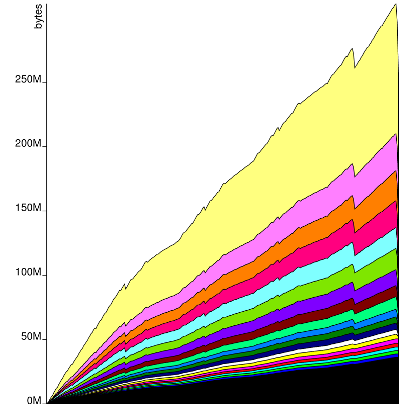
\includegraphics[width=\textwidth]{fig/nodiscard.png}
    \caption{Keeping all results and traces in memory.}
  \end{subfigure}
  \begin{subfigure}{0.49\textwidth}
    \centering
    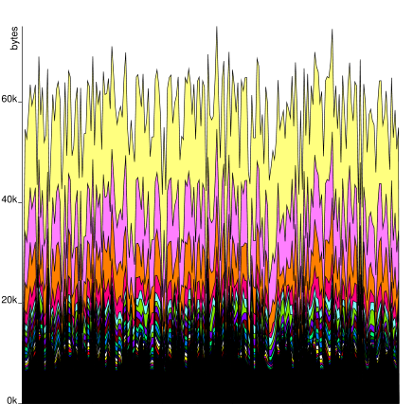
\includegraphics[width=\textwidth]{fig/discard.png}
    \caption{Discarding all traces, just keeping results.}
  \end{subfigure}
  \caption[Heap profiles of a test case for \texttt{MVar} contention.]{Heap profiles of a test case for \texttt{MVar} contention.  Note the dramatic difference: 250M without discarding vs 60k with.  These plots are intended to be viewed with colour.}\label{fig:discard}
\end{figure}

Tweag I/O\footnote{\url{http://www.tweag.io/}}, a research and
development company based in Paris, are using \dejafu{} as part of
their work on a distributed system for the SAGE
project\footnote{\url{http://www.sagestorage.eu/}}, which is
investigating storage systems for future supercomputers.  They cannot
share details of their work for commercial reasons, but one developer
had this to say (emphasis mine):

\begin{displayquote}
  Regarding the test case: we have an implementation of a distributed
  storage cluster, with possibly many nodes and parallel requests.
  The storage system itself is composed of several layers, which can
  be stacked on top of one another.  There is a lot of asynchronicity
  involved.  As per the tests themselves, I am testing parallel
  requests over different objects, etc.

  \emph{I'd like to add that dejafu tests are by far the most reliable
    tests in our suite, in my experience - I am yet to see a
    concurrency bug that they didn't spot, while some other tests
    missed them!} \parencite{tweag2017}
\end{displayquote}

\subsection{Richness of the Abstraction}

As we noted in \Cref{sec:dejafu-whatis-scope}, there are some areas
which we do not currently aim to support with \dejafu{}:

\begin{itemize}
\item Blocking a thread until a file descriptor becomes available, as
  this introduces an additional source of nondeterminism.
\item Throwing an exception to a thread if it becomes deadlocked, as
  we cannot reliably detect deadlock involving only a subset of
  threads without support from the garbage collector.
\item Querying which capability (OS thread) a Haskell thread is
  running on, as this introduces an additional source of
  nondeterminism.
\end{itemize}

These three areas are out of scope because we believe that the desire
for this functionality does not outweigh the implementation cost.  We
will look for a way, if that belief changes.

Introducing additional sources of nondeterminism into an SCT model is
difficult.  Simply introducing additional threads to model the
nondeterminism can cause an explosion of schedules tested, which is
unsatisfactory.  \verb|MonadConc| will always be limited to what
\dejafu{} can reasonably support.

However we can still push back the boundaries of what \dejafu{} supports.
Bound threads, Haskell threads which always run on the same unique OS
thread, were once out of scope as well.  This made it impossible to
use some C libraries with \verb|MonadConc|.  Now we have a prototype
implementation\footnote{\url{https://github.com/barrucadu/dejafu/issues/126}}
which shows promise, and which we intend to release.

\subsection{Writing and Porting Class-polymorphic Code}

\begin{listing}
\centering
\begin{cminted}{haskell}
instance MonadLogger (LoggerT STM) where -- ...
instance MonadLogger (LoggerT IO) where -- ...
\end{cminted}
\caption{Concrete instances for a typeclass-based logging abstraction.}\label{lst:mlogger1}
\end{listing}

We saw in the Par monad example that porting complex code to the
\verb|MonadConc| abstraction is not necessarily a difficult process.
However, this is not always the case.  Recently a user tried to port a
logging abstraction they made to \verb|MonadConc|.  Expressing this
with \verb|MonadConc| and \verb|MonadSTM| is not straightforward, as
constraints do not factor into instance selection.  So the instances
in \Cref{lst:mlogger2} overlap, and are illegal in standard Haskell.

\begin{listing}
\centering
\begin{cminted}{haskell}
instance MonadSTM  m => MonadLogger (LoggerT m) where -- ...
instance MonadConc m => MonadLogger (LoggerT m) where -- ...
\end{cminted}
\caption{Overlapping instances for a typeclass-based logging abstraction.}\label{lst:mlogger2}
\end{listing}

After some work, we introduced new \verb|IsSTM| and \verb|IsConc|
types to disambiguate between the two cases, and ended up with
\Cref{lst:mlogger3}.  The amount of effort required to arrive at this
solution led to the user questioning whether classes like their
\verb|MonadLogger| were even a useful abstraction at
all\footnote{\url{https://www.reddit.com/r/haskell/comments/7b1fbk/do_mtlstyle_effect_classes_really_pull_their/}}!
This is a good topic to think about, but it should not be prompted by
the effort of trying to use \dejafu{}.

\begin{listing}
\centering
\begin{cminted}{haskell}
instance MonadSTM  m => MonadLogger (LoggerT (IsSTM  m)) where -- ...
instance MonadConc m => MonadLogger (LoggerT (IsConc m)) where -- ...
\end{cminted}
\caption{Polymorphic instances for a typeclass-based logging abstraction.}\label{lst:mlogger3}
\end{listing}

So while porting code to the \verb|MonadConc| typeclass is often
simple when dealing with datatype and function definitions, it can be
more complicated when dealing with typeclasses.  It is not clear what
can be done to improve this matter.

\subsection{Library Alternatives}

There are popular Haskell libraries specifically for concurrency.  One
of these is the async library \parencite{async}, part of which we looked at
as a case study~\sref{dejafu-casestudies-async}, for expressing
asynchronous computations.  This library is intended to be a
higher-level and safer way of expressing asynchronous computations
with guaranteed cleanup than using threading, mutable state, and
asynchronous exceptions directly.

Our concurrency library, which provides \verb|MonadConc|, includes an
alternative to async using \verb|MonadConc|.  There is a test suite
using \dejafu{}.  The test suite for async itself just runs most tests
a single time, although one of them is run 1000 times.  Using
\dejafu{} here to automatically seek out interesting schedules is a
much more principled approach then repetition and hope.  Not all
features of async are supported, however.  As we do not currently
support bound threads, functions that use them have been omitted.

This is just one library, and providing an alternative library that
people will have to switch to is far from optimal.  However, until
library authors start to use \dejafu{} and \verb|MonadConc| directly,
such alternatives will be needed to answer the question `Why should I
use this if I cannot use it with anything I use already?'

\subsection{Tool Integration}

There are two popular libraries for unit testing in Haskell,
HUnit \parencite{hunit} and Tasty \parencite{tasty}.  From the perspective of the
user, the libraries are similar, but from the perspective of the
implementer, they have different approaches to integration.  The
hunit-dejafu \parencite{hunit_dejafu} and tasty-dejafu \parencite{tasty_dejafu}
packages provide integration with both.

These packages provide analogues of the \dejafu{} functions, but using
the interface of the testing frameworks, rather than computing and
printing results directly.  The test-framework \parencite{test_framework}
library is also in common use, however it supports integration with
HUnit, and so needs no special support of its own.

The Tasty library is more featureful than HUnit, supporting progress
reporting, giving a message on success as well as failure, and
command-line arguments.  The tasty-dejafu package is similar to the
hunit-dejafu package and does not make use of these additional
features.

\vfill\pagebreak
\section{Summary}

In this chapter we presented \dejafu{}, our tool for testing
concurrent Haskell programs:

\begin{itemize}
\item We provide a typeclass abstraction over concurrency.  Such an
  abstraction allows \verb|IO| to be swapped out and replaced with
  another implementation~\sref{dejafu-monadconc}.

\item We implemented a model of Haskell
  concurrency~\sref{dejafu-execution}, with an empirically derived
  operational semantics~\sref{dejafu-semantics}, so that we can
  simulate the behaviour of GHC.  Our model includes most of the
  Control.Concurrent library module, although some operations are out
  of scope, or have their behaviour changed~\sref{dejafu-whatis-scope}.

\item We use bounded partial-order reduction \parencite{coons2013} with
  relaxed memory \parencite{zhang2015} as the core testing algorithm for
  \dejafu{}, but also support a controlled random scheduling
  approach~\sref{dejafu-testing}.

\item We have not attempted a formal proof of correctness of
  \dejafu{}, but have made an informal correctness argument, noting
  the limits of how correct \dejafu{} can be.  We do have a
  comprehensive test suite, and check what correctness conditions we
  can~\sref{dejafu-correctness}.

\item We have discussed three case studies, all of which involved
  applying \dejafu{} to pre-existing code.  Such code must be modified
  to use the \dejafu{} typeclass abstraction, but we have found this
  to be a straightforward and type-directed process in most
  cases~\sref{dejafu-casestudies}.
\end{itemize}

Although a commonly reported experience amongst Haskell programmers is
that ``if it compiles, it works,'' there are times when it does
\emph{not} work.  Concurrency is a particularly difficult area to get
right, as everyone who has had to move outside the realm of guaranteed
determinism will know.  By developing \dejafu{}, we hope that
concurrency in Haskell will become a little easier to get right.

\paragraph{Context}
\dejafu{} does not stand alone, it is related to our other
contributions:

\begin{itemize}
\item \Cref{chp:algorithms} discusses a new random scheduling
  algorithm for incomplete concurrency testing.  The chapter does not
  directly build on \dejafu{}, but \dejafu{} implements the algorithm.
\item \Cref{chp:coco} discusses a new property-discovery tool for
  functions operating on mutable state.  The tool directly builds on
  \dejafu{} in two ways: (1) to discover these properties, and (2) by
  providing an interface for \dejafu{} to check them.
\end{itemize}


\chapter{Scheduling Algorithms}
\label{chp:algorithms}
We have seen that the complete-within-a-bound approach of DPOR is not
suitable for some programs.  Programs with large state-spaces, or with
sources of nondeterminism other than the scheduler, pose a problem.
One way to address this is to sacrifice completeness, and instead
explore the space of schedules \emph{randomly}.  We may not find all
bugs.  However we still want to find \emph{most of them}.  Benchmarks
show that some scheduling algorithms tend to be better at this than
others; not all algorithms are created equal.  In this chapter we
discuss two different randomised scheduling
algorithms~\sref{algorithms-usual} and then propose a new one based on
a \emph{weighted} random selection of threads~\sref{algorithms-swarm}.
We show that our proposed algorithm performs favourably in a
comparison of standard benchmark programs~\sref{algorithms-bench}, and
evaluate the approach~\sref{algorithms-eval}.

\section{Concurrency Testing with Randomised Scheduling}
\label{sec:algorithms-usual}

Concurrency testing using randomised scheduling works by repeatedly
executing a concurrent program, exploring a particular schedule on
each execution.  Unlike systematic testing, these algorithms are
incomplete in general, and little effort is made to avoid repetition
of schedules.  In this section we present two approaches to randomised
scheduling.

\paragraph{Controlled random scheduling}
A controlled random scheduler uses a pseudorandom number generator to
choose threads to execute.  At each scheduling point, a runnable
thread is selected at random.  This thread is then executed until the
next scheduling point.  Like any controlled scheduling technique, the
executed schedule can be recorded and replayed.  Additionally, a
controlled random scheduler can be used on programs that exhibit
nondeterminism beyond scheduler nondeterminism, although in this case
schedule replay will be unreliable \parencite{thomson2016}.

\paragraph{Probabilistic concurrency testing}
The PCT algorithm \parencite{burckhardt2010} is a randomised algorithm
with a probabilistic guarantee of finding bugs.  Key to its design is
a notion of the \emph{depth} of a bug: the minimum number of
scheduling constraints required to exhibit it.  The intuition behind
PCT is that most concurrency bugs can be exhibited with just a few
scheduling decisions being made in the correct places, or the
incorrect places depending on your point of view.  If PCT makes those
decisions correctly, it finds the bug regardless of what any other
scheduling decisions were.

On each execution, PCT focuses on finding bugs of a particular depth
$d$.  PCT uses a priority-based scheduler where the highest-priority
runnable thread is scheduled at each point.  $d$ priority change
points are distributed randomly through the execution, which is why we
must know the length, $k$, of the program.  When execution reaches a
change point, the priority of the currently executing thread is
changed to a low value.

The algorithm proceeds as follows; given a program with at most $n$
threads and at most $k$ steps, choose a depth $d$, then:

\begin{enumerate}
\item Randomly assign each of the $n$ threads a distinct priority
  value from $\{d, d + 1, \ldots, d+n\}$.  The lower priority values
  $\{1, \ldots, d−1\}$ are reserved for change points.
\item Randomly pick integers $c_1, \ldots, c_{d−1}$ from
  $\{1, \ldots, k\}$.  These will be the priority change points.
\item Schedule threads strictly according to their priorities: never
  schedule a thread if a higher priority thread is runnable.  After
  executing the $c_i$-th step $(1 \leq i < d)$, change the priority of
  the thread that executed the step to $i$.
\end{enumerate}

In a single run of a program with $n$ threads and $k$ steps, PCT finds
a bug of depth $d$ with probability at least $1/nk^{d−1}$.

\paragraph{Dynamic partial-order reduction}
The algorithms we discuss in this chapter are \emph{alternatives} to
DPOR.  They are useful when the program is too big for a complete
approach, even with schedule bounding, and so exploring a
representative sample of executions is all we have left.

There is another approach: combining randomisation with DPOR.
\cite{sen2007} proposes the RAPOS algorithm, which uses DPOR to prune
the search space, and then explores a random subset of the partial
orders discovered.  They show that this approach samples different
partial orders more uniformly than a simple randomised scheduler, and
so it is likely to discover faulty executions more reliably.

\section{Weighted Random Scheduling and Swarm Testing}
\label{sec:algorithms-swarm}

We now present \emph{swarm scheduling}, our new algorithm for finding
concurrency bugs with controlled scheduling.  The algorithm is
inspired by \emph{swarm testing} \parencite{groce2012}, an approach to
finding bugs using random testing more effectively.  Swarm testing
makes the observation that, in a random testing tool with many
available choices, a uniform distribution is unlikely to discover bugs
which correspond to an unfair result:

\begin{displayquote}
  As a simple example, consider testing an implementation of a stack ADT that
  provides two operations, push and pop. [\ldots] To make this example more
  interesting, imagine the stack implementation has a capacity bug, and will
  crash whenever the stack is required to hold more than 32
  items. \parencite{groce2012}
\end{displayquote}

The authors then argue that tests generated by randomly interleaving
push and pop operations are unlikely to produce a stack with more than
32 items, as items would tend to be popped as quickly as they are
pushed.  The proposed alternative is, rather than having a
\emph{single} distribution for all tests, generate \emph{multiple}
distributions to encourage greater variety.

We transfer this idea to the context of scheduling algorithms by
observing that controlled random scheduling is much like using a
single distribution to generate random tests.  So instead, we assign a
randomly chosen \emph{weight} to each new thread as it is created, and
schedule threads with a weighted random selection.  This approach is
similar to PCT, but less deterministic: PCT will always schedule the
highest-weighted runnable thread, whereas our approach is most likely
to, but may not.  We can also introduce change points, as in PCT,
where we assign the currently executing thread a new weight.

With weight change points included, the algorithm is as follows: given a program
with at most $k$ steps, choose a range of weights $[w_{min}, w_{max}]$ and
a bound $d$, then:

\begin{enumerate}
\item Assign the initial thread a weight from $[w_{min}, w_{max}]$.
\item Randomly pick integers $c_1, \ldots, c_{d-1}$ from $\{1, \ldots, k\}$.
These will be the weight change points.
\item Schedule threads by a weighted random selection: at each scheduling point
use the weights of the enabled threads to construct a nonuniform distribution
and pick a thread to run until the next scheduling point.  As new threads are
created, assign a weight from $[w_{min}, w_{max}]$.  After executing
the $c_i$-th step $(1 \leq i < d)$, change the weight of the thread that
executed the step to a random value from $[w_{min}, w_{max}]$.
\end{enumerate}

\dejafu{} has a Haskell implementation of swarm scheduling and of
controlled random scheduling using a uniform distribution, where the
latter is treated as a special case of swarm scheduling where
$w_{min} = w_{max}$.

\section{Comparing Bug-finding Ability}
\label{sec:algorithms-bench}

We shall now see how swarm scheduling compares with PCT in terms of
bug-finding ability.  We use a published collection of benchmark
programs, SCTBench \parencite{thomson2016,thomson2014}, and a modified
version of the Maple tool \parencite{yu2012}.  Maple is a tool for testing
Linux programs which use POSIX threads \parencite{ieee1995}.  We use Maple
because the prior work using SCTBench also does.  We want any
difference in algorithm performance to be due to the algorithms
themselves, not because of any difference in how the host tool works.

Maple comes with a PCT implementation using Linux real-time thread
priorities, but we use the modified version from \cite{thomson2016}
instead.  This modified version differs from the standard PCT
algorithm slightly.  PCT does not directly handle yielding threads: if
the highest-priority runnable thread is in a busy-wait loop, it may
yield until some condition holds.  Immediately scheduling the thread
again after it yields would lead to a nonterminating execution.  The
original PCT implementation uses heuristics to determine if a thread
is not making progress, and to lower its priority
\parencite{burckhardt2010}.  In the implementation we use, the
priority of a yielding thread is changed to the lowest priority.

\subsection{Benchmark Collection}
\label{sec:algorithms-bench-sctbench}

SCTBench \parencite{thomson2016,thomson2014} is a collection of pthread
programs amenable to concurrency testing by controlled scheduling.
All the programs are deterministic, other than scheduler
nondeterminism.  In total there are 49 benchmark programs.  SCTBench
is assembled from several other sets of benchmarks, so there is some
variety in the programs:

\begin{itemize}
\item Buggy versions of aget (a file downloader) and pbzip2 (a compression
program).
\item A set of test cases for a work-stealing queue.
\item Examples used to test the ESBMC tool \parencite{cordeiro2011}, an SMT-based
model checker for concurrency.
\item Examples used to test the INSPECT tool \parencite{yang2008}, a concurrency
testing tool for instrumented C programs.
\item A buggy lock-free stack implementation.
\item A test case exposing a bug in the ctrace \parencite{mcpherson2003}
  concurrency debugging library.
\item Buggy versions of a content similarity search tool and online clustering
tool.
\item Three benchmarks exposing bugs in Mozilla
  SpiderMonkey \parencite{eich1996} and the Mozilla Net\-scape Portable
  Runtime Thread Package \parencite{mozilla1996}.
\item The SPLASH-2 programs \parencite{woo1995}.
\end{itemize}

\subsection{Experimental Method}
\label{sec:algorithms-bench-method}

We aim to compare swarm scheduling, using a variety of parameters, with PCT and
controlled random scheduling.  We do not consider the other algorithms used in
the prior SCTBench work, or PCT with a bound other than $d=3$, as setting $d=3$ was
found to give the best results in terms of bug-finding ability \parencite{thomson2016}.

In total, we try 5 algorithm-parameter variants:

\begin{itemize}
\item Controlled random scheduling.
\item PCT with $d=3$.
\item Swarm scheduling with $d \in \{1,2,3\}$.
\end{itemize}

For each variant, we run each benchmark with a limit of 10,000
executions.  We use a schedule limit rather than a time limit, as many
factors can influence timing results, and they are not readily
comparable or reproducible.  Number of executions required, however,
is an intrinsic property of the benchmark program, the testing
algorithm, and any parameters.

We were fortunate enough to have access to the scripts used
by \cite{thomson2016} to run the benchmarks, which greatly
simplified experimentation.  Each benchmark goes through each of the
following phases of testing:

\paragraph{Data race detection phase}
It is sound to only consider scheduling points before synchronisation operations
as long as execution aborts with an error as soon as a data race is
detected \parencite{musuvathi2008}.  This greatly reduces the number of schedules that
need to be considered.  However, the benchmark programs contain many benign data
races \parencite{thomson2016}, so this condition is too strict.  As in prior
work \parencite{thomson2016,thomson2014,yu2012} we address this problem by performing
dynamic data race detection first, to identify a subset of load and store
operations which are known to be racey, which are then treated as visible
synchronisation operations during testing.  This process is nondeterministic, so
we run it ten times for each benchmark.

\paragraph{Controlled random scheduling phase}
We run each benchmark 10,000 times using Maple's controlled random scheduler.  Although
this approach was found to be inferior to PCT \parencite{thomson2016}, we include it
so we have a na\"{\i}ve baseline for evaluation purposes.

\paragraph{PCT testing phase}
PCT requires parameters $n$, the maximum number of threads; $k$, the maximum
number of steps in the execution; and $d$, the bug depth.  We fix $d=3$, and use
estimates for $n$ and $k$ found by \cite{thomson2016}.  These estimates were
obtained by making an initial estimate and then executing PCT with $d=3$, on the
assumption that this would increase interleaving, and counting steps from when
the first thread launches the second.  We run each benchmark 10,000 times using
its estimated $n$ and $k$ values.

\paragraph{Swarm scheduling phase}
Swarm scheduling requires parameters $w_{min}$, the minimum weight;
$w_{max}$, the maximum weight; $k$, the maximum number of steps in the
execution; and $d$, the number of weight change points to include.  We
want to encourage executions with very unequal thread weights, and so
pick $w_{min}=1$ and $w_{max}=50$, giving significantly more weights
than most benchmarks have threads.  We use the same $k$ values as in
PCT.\@ We then perform multiple runs of swarm scheduling: we perform
10,000 executions of each benchmark program for each $d$, using its
estimated $k$ value.

\paragraph{Note on randomness}
For a given benchmark, we can use the average number of schedules
needed to expose a bug (10,000 $\div$ the number of buggy schedules)
to compare techniques.  The exact value is dependent on the initial
seed, but we would expect it to become stable as the number of
executions is increased \parencite{thomson2016}.

\begin{figure}
  \centering
  \begin{subfigure}{0.3\textwidth}
    \centering
    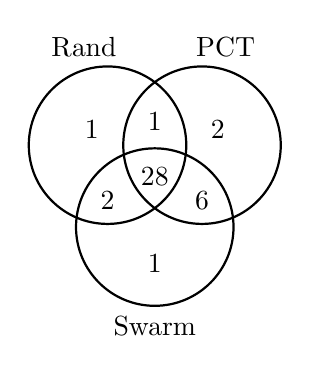
\begin{tikzpicture}[thick]
      \draw (0,0)      circle (1) node[above,shift={(-0.3,1)}] {Rand};
      \draw (1.2,0)    circle (1) node[above,shift={(0.3,1)}]  {PCT};
      \draw (.6,-1.04) circle (1) node[below,shift={(0,-1)}]   {Swarm};

      \node at (.6,-.4)  {28}; % rand  ^ pct   ^ swarm
      \node at (1.2,-.7) {6};  % pct   ^ swarm - rand
      \node at (.6,.3)   {1};  % pct   ^ rand  - swarm
      \node at (0,-.7)   {2};  % rand  ^ swarm - pct
      \node at (1.4,.2)  {2};  % pct   - rand  - swam
      \node at (-.2,.2)  {1};  % rand  - pct   - swarm
      \node at (.6,-1.5) {1};  % swarm - pct   - rand
    \end{tikzpicture}
    \caption{Basic algorithms}\label{fig:bugs-base}
  \end{subfigure}
  \begin{subfigure}{0.3\textwidth}
    \centering
    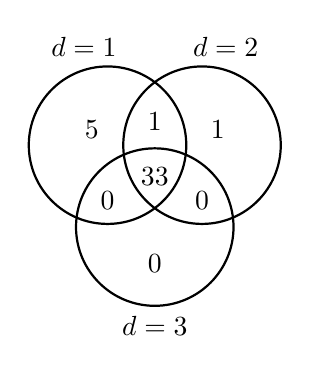
\begin{tikzpicture}[thick]
      \draw (0,0)      circle (1) node[above,shift={(-0.3,1)}] {$d=1$};
      \draw (1.2,0)    circle (1) node[above,shift={(0.3,1)}]  {$d=2$};
      \draw (.6,-1.04) circle (1) node[below,shift={(0,-1)}]   {$d=3$};

      \node at (.6,-.4)  {33}; % 1 ^ 2 ^ 3
      \node at (0,-.7)   {0};  % 1 ^ 3 - 2
      \node at (.6,.3)   {1};  % 1 ^ 2 - 3
      \node at (1.2,-.7) {0};  % 2 ^ 3 - 1
      \node at (-.2,.2)  {5};  % 1 - 2 - 3
      \node at (1.4,.2)  {1};  % 2 - 1 - 3
      \node at (.6,-1.5) {0};  % 3 - 1 - 2
    \end{tikzpicture}
    \caption{Weight changes}\label{fig:bugs-swarmd}
  \end{subfigure}

  \caption{Overlap of bugs found by each scheduling algorithm.}\label{fig:bugs}
\end{figure}

\subsection{Experimental Results}
\label{sec:algorithms-bench-results}

We conducted our experiments using an Ubuntu 12.04 virtual machine,
and a modified version of Maple based on the last commit from
2012\footnote{The same environment as \cite{thomson2016}, available at
  \url{https://github.com/mc-imperial/sctbench}}.  \Cref{lst:swarm} in
\Cref{app:swarm} shows the core of our C++ swarm scheduling
implementation.  Other than the addition of swarm scheduling, the code
is unchanged.

The Venn diagrams in \Cref{fig:bugs} show the relative bug-finding
ability of each algorithm.  \Cref{fig:bugs-base} summarises the bugs
found by controlled random scheduling, PCT $d=3$, and swarm scheduling
$d=0$ (which we now call ``Swarm'' for brevity).  Swarm performs
comparably with PCT.  \Cref{fig:bugs-swarmd} shows the effect of
introducing weight change points, which seems to harm performance.

\begin{figure}
  \centering
  \input{gen/bugs.tex}
  \caption[Plot of bugs found by each scheduling algorithm.]{The number of bugs found by each algorithm across all benchmarks.  This plot is intended to be viewed with colour.}\label{fig:totalbugs}
\end{figure}

As the techniques we have considered are nondeterministic, it is
interesting to consider their average-case behaviour.
\Cref{fig:totalbugs} shows the aggregate behaviour of the algorithms
across all benchmarks as the number of executions increases.  Swarm
outperforms PCT at first, but PCT catches up as the number of
executions increases.

\begin{figure}
  \centering
  \begin{subfigure}{0.49\textwidth}
    \centering
    \resizebox{\textwidth}{!}{\input{gen/freqs-total.tex}}
    \caption{All buggy executions.}\label{fig:freqbugs-total}
  \end{subfigure}
  \begin{subfigure}{0.49\textwidth}
    \centering
    \resizebox{\textwidth}{!}{\input{gen/freqs-unique.tex}}
    \caption{Unique buggy executions.}\label{fig:freqbugs-unique}
  \end{subfigure}
  \caption[Plot of average number of executions needed to expose a bug.]{The average number of executions to expose a bug across all benchmarks.  These plots are intended to be viewed with colour.}\label{fig:freqbugs}
\end{figure}

The plots in \Cref{fig:freqbugs} show the average number of executions
to find a bug across all benchmarks; as expected, the average number
of executions to find \emph{any} bug rapidly converges, however the
average number of schedules to find a \emph{unique} bug does not.
This is due to two factors: (1) the number of bugs is finite; and (2)
some bugs may be out of reach of a particular algorithm.
\Cref{tbl:freqs} shows the final values.  We can see that PCT and
Swarm are almost identical, and both significantly improve upon random
scheduling when it comes to finding unique bugs.

\begin{table}
  \centering
  \begin{tabular}{lrr} \toprule
    Algorithm & Any Bug & A Unique Bug \\ \midrule
    Random & 0.071 & 312.5 \\
    PCT   & 0.077 & 270.3 \\
    Swarm & 0.078 & 270.3 \\ \bottomrule
  \end{tabular}
  \caption{Average number of executions needed to find a bug.}\label{tbl:freqs}
\end{table}

\section{Evaluation}
\label{sec:algorithms-eval}

Testing concurrent programs by using a swarm of randomly generated
weighted distributions appears to work well in practice.  The simplest
variant, which we simply call Swarm, uses no weight change points.  So
for Swarm, the $k$ and $d$ parameters are irrelevant, which means the
user does not need to know the maximum length of their program
execution in advance.  Although it is disappointing that Swarm does
not improve upon PCT, in terms of bug-finding it does perform
comparably.

A significant advantage of the Swarm method over PCT is that it does
not require the programmer to first determine the maximum length of an
execution, which can be difficult to estimate.

\paragraph{Randomised stride}
Another algorithm with a similar motivation is the randomised stride
algorithm \parencite{abdelrasoul2017}, which outperforms PCT (and so our
Swarm algorithm).  This is a recent algorithm which was not yet
published when we began this work.  Like PCT, randomised stride
derives its power from knowledge of the underlying program: in this
case, an estimate of the length of each thread.  Although Swarm
performs worse than randomised stride, we believe it still has a place
in the concurrency testing arsenal as an effective algorithm which
does not require first estimating or measuring some parameter of the
program under test.

\paragraph{Why are weight changes bad?}
\Cref{fig:bugs-swarmd} shows that, although using one weight change
point results in finding an additional bug, bug-finding ability
rapidly degrades as more points are introduced.  We suspect that this
is because frequent weight changes compromise the intuition for why
weighted random testing is effective at all.  We believe that weighted
random testing is effective because unfair scheduling causes threads
to make progress at different rates, leading to interleavings which
the programmer is unlikely to have considered.  However, by changing
weights, a thread which was previously making rapid progress may
suddenly slow down, allowing other threads to catch up.  In the
extreme, if we introduce a weight change after every scheduling point,
we have simply produced a complicated version of uniform random
scheduling.

\section{Summary}

In this chapter we presented swarm scheduling, our scheduling
algorithm for finding faults in concurrent programs:

\begin{itemize}
\item We propose that unfair schedules are likely to reveal
  concurrency bugs more effectively than fair schedules.  Unfair
  schedules cause different threads to make progress at different
  rates, resulting in interleavings the programmer is unlikely to have
  considered~\sref{algorithms-eval}.

\item Swarm scheduling uses weighted random scheduling, with optional
  weight change points.  However, frequently changing the weights
  causes weighted scheduling to degrade to an effectively uniform
  scheduling~\sref{algorithms-swarm}.

\item We find that one parameterisation of the swarm scheduling
  algorithm performs as well as PCT \parencite{burckhardt2010}, despite not
  knowing anything about the program under test.  We argue that this
  makes swarm scheduling easier to use, while giving just as good
  results~\sref{algorithms-bench}.
\end{itemize}

The complete systematic approach to testing is not necessarily
suitable for all programs.  Programs with large state-spaces, or
programs which have sources of nondeterminism other than the
scheduler, cannot readily be tested with such techniques.  For such
programs, random testing is commonly used.  By introducing swarm
scheduling, we hope that effective random testing of concurrent
programs will become simpler.

\paragraph{Context}
Swarm does not stand alone, it is related to our other contributions:

\begin{itemize}
\item \Cref{chp:dejafu} uses swarm scheduling to provide its random
  testing mode.  Complete testing is the default.  Swarm scheduling
  was added for cases where the state-space is too large to
  systematically explore.
\end{itemize}


\part{Test Case Generation}
\label{part:properties}

\chapter{CoCo: Discovering Properties Automatically}
\label{chp:coco}
In this chapter we present and evaluate CoCo, our tool for finding
properties of equivalence and refinement between concurrent Haskell
expressions with shared state.  We first discuss some key concerns in
the implementation of a tool like this~\sref{coco-concerns}, and then
demonstrate the use of the tool with an illustrative
example~\sref{coco-example}.  We explain how properties are
discovered~\sref{coco-hiw} and argue the correctness of our
approach~\sref{coco-correctness}.  We then present two further
examples~\sref{coco-cases}.  Next we discuss how CoCo properties can
be incorporated into a \dejafu{} test suite~\sref{coco-dejafu}.
Finally, we present conclusions and evaluate the
approach~\sref{coco-conclusions}.

This chapter is derived from our previous work \cite{tfp-coco} and
\cite{flops-coco}.

\section{Key Concerns of Observing Concurrent Programs}
\label{sec:coco-concerns}

In implementing a tool to discover properties of \emph{concurrent}
programs, we have some concerns which are not applicable to sequential
programs.  Firstly, concurrent programs are nondeterministic; so if we
simply compared results of single executions, the discovered
properties may not hold in the general case.  Secondly, mutable state
is subject to interference from other threads; so if we do not
consider concurrent interference, the discovered properties may not
hold when there are more threads involved.  Finally, we need to decide
what it means for two concurrent programs to be related.

\paragraph{Nondeterminism}
If we restrict the nondeterminism in our program to schedule
nondeterminism, we can use systematic concurrency testing
(SCT)\cite{coons2013,flanagan2005,musuvathi2008,musuvathi2007}
techniques as implemented in \dejafu{}, discussed in
\Cref{chp:dejafu}, to produce the set of results of a generated
program fragment.

\paragraph{Interference}
We do not know what sort of interference may lead to interesting
results.  So CoCo requires the programmer to supply a function with
effects, which is executed concurrently during property discovery, to
provide this interference.  By supplying different sorts of
interference, the programmer can see how the functions under test
behave in different concurrent contexts.

\paragraph{Properties}
We formulate our properties in terms of \emph{observational
  refinement}\cite{he1986}, where the observations we take are
snapshots of the state.  CoCo requires the programmer to supply an
observation function to produce these snapshots.  By varying their
observation function, the programmer can see different aspects of the
functions under test.

We define a \emph{behaviour} of a concurrent program as a pair of a
final observation, taken after the program terminates, and a possible
failure.  By considering the set of a program's possible behaviours,
rather than simply final observations, we can distinguish between
operations which may fail and those which do not.  Properties that we
report are of the form \verb|A === B|, meaning that the sets of
behaviours of \verb|A| and \verb|B| are equal; and \verb|A ->- B|,
meaning that the set of behaviours of \verb|A| is a strict subset of
the set of behaviours of \verb|B|.

\section{An Illustrative Example}
\label{sec:coco-example}

Let us now show an example use of CoCo for Haskell \verb|MVar|s.
Recall that an \verb|MVar| is a mutable memory cell which may be
\emph{full} or \emph{empty}.  We now examine three basic operations
over \verb|MVar|s: put, take, and read.  To \emph{put} is to block
until the \verb|MVar| is empty and then set its value.  To \emph{take}
is to block until the \verb|MVar| is full, remove its value, and
return the value.  To \emph{read} is to \emph{take}, but without
emptying the \verb|MVar|.  Each function has a non-blocking \emph{try}
variant, which returns an indicator of success.

\begin{listing}
\centering
\begin{cminted}{haskell}
putMVar  :: MVar Concurrency Int -> Int -> Concurrency ()
takeMVar :: MVar Concurrency Int -> Concurrency Int
readMVar :: MVar Concurrency Int -> Concurrency Int
\end{cminted}
\caption{Type signatures for \texttt{MVar} operations in CoCo.}\label{lst:mvar_types}
\end{listing}

Allowing shared values of type \verb|Int|, we obtain the type
signatures in \Cref{lst:mvar_types}.  Here \verb|Concurrency| is an
implementation of the \verb|MonadConc| typeclass from
\Cref{chp:dejafu}, provided by CoCo.  The \verb|MVar| type is an
abstract type defined in \verb|MonadConc|, with the concrete type
determined by the monad used.  In this case the concrete type is
defined as part of \dejafu{}.

\begin{listing}
\centering
\begin{cminted}{haskell}
type C = Concurrency

sig :: Sig (MVar C Int) (Maybe Int) (Maybe Int)
sig = Sig
  { initialise  = maybe newEmptyMVar newMVar
  , expressions =
    [ -- example 1
      lit "putMVar"  (putMVar  :: MVar C Int -> Int -> C ())
    , lit "takeMVar" (takeMVar :: MVar C Int -> C Int)
    , lit "readMVar" (readMVar :: MVar C Int -> C Int)
    ]
  , backgroundExpressions =
    [ -- example 2
      lit "tryPutMVar" (tryPutMVar :: MVar C Int -> Int -> C Bool)
    ]
  , interfere  = \v _ -> putMVar v 42
  , observe    = \v _ -> tryReadMVar v
  , backToSeed = \v _ -> tryReadMVar v
  }
\end{cminted}
\caption{CoCo signature for \texttt{MVar}s holding \texttt{Int}s.}\label{lst:mvar}
\end{listing}

\paragraph{Signatures}
When we use CoCo, we must provide four things: (1) the functions and
values which may appear in properties; (2) a way to initialise the
state; (3) an observation function; and (4) an interference function.

We call this collection of programmer-supplied definitions the
\emph{signature}.  \Cref{lst:mvar} shows a signature for \verb|MVar|
operations.  The initialisation function constructs an empty or a full
\verb|MVar|.  The interference function simply stores a new value.
The observation function takes a snapshot of the state.  The
\verb|backToSeed| function is used to check whether the state has been
changed: if the original and final seed values are the same, the state
is unchanged.

It is essential to provide an initialisation function which gives a
representative collection of states, and an interference function
which can disrupt the functions of interest.  If our initialisation
function only produced a full \verb|MVar|, we could find properties
which do not hold when the \verb|MVar| is empty.  Because our
interference function only writes to the \verb|MVar|, we may find
properties which do not hold when there are multiple consumers.
Developing a fuller understanding of the functions under test may
require examining the different property-sets found under different
execution conditions.

\paragraph{Discovering properties}
\Cref{lst:mvar_props1} shows the properties which CoCo discovers given
the signatures in \Cref{lst:mvar}.  In this output, \verb|@| is the
state argument, which is the \verb|MVar|.  For convenience of
reference, we have added numbers to the CoCo properties.  These
numbers are not included in the normal output of the tool.

\begin{listing}
\centering
\begin{cminted}{text}
(1)   readMVar @  ===  readMVar @ >> readMVar @
(2)   readMVar @  ->-  takeMVar @ >>= \x -> putMVar @ x
(3)   takeMVar @  ===  readMVar @ >> takeMVar @
(4)  putMVar @ x  ===  putMVar @ x >> readMVar @
\end{cminted}
\caption{CoCo-discovered properties about \texttt{MVar}s.}\label{lst:mvar_props1}
\end{listing}

Property (1) shows that \verb|readMVar| is idempotent; (2) shows that
it is not merely a take followed by a put, it is rather a distinct
operation; (3) and (4) show that it does not modify the \verb|MVar|,
and that it does not block when the \verb|MVar| is full.  Property (4)
may appear to be type-incorrect, but remember that CoCo does not
consider equality of term results, only the effects.

\begin{table}[t]
\centering
\begin{tabular}{p{7.5em}p{7.5em}p{7.5em}p{7.5em}} \toprule
  Term       & Seed           & Final State & Deadlocks \\ \midrule
  Read       & \verb|Nothing| & \verb|Just 42| & No  \\
             & \verb|Just 0|  & \verb|Just 0|  & No  \\
  Take / Put & \verb|Nothing| & \verb|Just 42| & No  \\
             & \verb|Just 0|  & \verb|Just 0|  & No  \\
             &                & \verb|Just 42| & Yes \\ \bottomrule
\end{tabular}
\caption{The behaviours of the terms in property (2).}
\label{tbl:behaviours}
\end{table}

We see the effect of the interference in (2): with no other producers,
this would be an equivalence; it is only when interference by another
thread is introduced that the equivalence breaks down and the
distinction is revealed.  \Cref{tbl:behaviours} shows the possible
behaviours.  This property is a strict refinement because, while the
behaviours for the seed value \verb|Nothing| are the same, the
behaviours of the left term for the seed value \verb|Just 0| are a
strict subset of the behaviours of the right.

\paragraph{Background expressions}
Sometimes when expressing properties it is necessary to call upon
other expressions which are of secondary interest.  Such expressions
are commonly called \emph{background} expressions.  A property is only
reported if each side includes at least one non-background expression.

\begin{listing}
\centering
\begin{cminted}{text}
      readMVar @  ===  readMVar @ >> tryPutMVar @ x
(5)   readMVar @  ===  readMVar @ >>= \x -> tryPutMVar @ x
      readMVar @  ->-  takeMVar @ >>= \x -> tryPutMVar @ x
     putMVar @ x  ===  putMVar @ x >> tryPutMVar @ x1
\end{cminted}
\caption{Additional CoCo-discovered properties about \texttt{MVar}s.}\label{lst:mvar_props2}
\end{listing}

If we include \verb|tryPutMVar|, a non-blocking version of
\verb|putMVar|, as a background expression, CoCo discovers the
additional properties in \Cref{lst:mvar_props2}.  Property (5) shows
how important the choice of interference function is.  The left and
right terms are not equivalent.  If the interference were to empty a
full \verb|MVar| then the right term could restore its original value.
As our choice of interference function only produces, rather than
consumes, it will never alter the value in a full \verb|MVar|.

The example in this section takes about 1.5 seconds to run, and the
output displayed here is the output of the tool, aside from the
property numbers.  We discuss further performance results in
\Cref{sec:coco-conclusions}.

\section{How CoCo Works}
\label{sec:coco-hiw}

A simplified version of our approach is to generate all terms up to
some syntactic size limit, compute and store their behaviours, and
then find properties by comparing the sets of behaviours of each pair
of terms.  This would be slow, however.  Following the lead of
QuickSpec\cite{claessen2010,smallbone2017} we make three key
improvements:

\begin{enumerate}
\item We generate \emph{schemas} with \emph{holes}, rather than
  \emph{terms} with \emph{variables}.
\item We only compute the set of behaviours of the most general term
  of every schema.
\item We interleave property discovery with schema generation, and
  aggressively prune redundant schemas.
\end{enumerate}

The main difference between our approach and QuickSpec is how we
handle monadic operations, and that QuickSpec compares \emph{equality}
of term \emph{results} whereas we compare \emph{refinement} of term
\emph{behaviours}.  Furthermore, we generate lambda-terms in a
restricted setting whereas QuickSpec does not do so at all.

\subsection{Representing and Generating Expression Schemas}
\label{sec:coco-hiw-gen}

We can greatly reduce the number of expressions considered by not
generating alpha-equivalent ones.  Instead of generating an expression
like \verb|push @ x >> push @ y|, we will instead generate the
expression \verb|push @ ? >> push @ ?| where each \verb|?| is a
\emph{hole} for a variable.  These expressions-with-holes are called
\emph{schemas}.  One schema can be instantiated into many \emph{terms}
by assigning variable names to groups of holes.  The push-push schema
has two semantically distinct term instances: the single-variable and
the two-variable cases.

\begin{listing}
\centering
\begin{cminted}{haskell}
data Expr s h
  = Lit  String Dynamic
  | Var  TypeRep (Var h)
  | Bind TypeRep (Expr s h) (Expr s h)
  | Ap   TypeRep (Expr s h) (Expr s h)
  | State

data Var h = Hole h | Named String | Bound Int

type Schema s = Expr s ()
type Term   s = Expr s Void
\end{cminted}
\caption{Representation of Haskell expressions.}
\label{lst:exprrep}
\end{listing}

Our expression representation is shown in \Cref{lst:exprrep}.  The
\verb|Expr| type is parameterised by a state type \verb|s| and a
\emph{hole} type \verb|h|.  The state parameter ensures expressions
that assume different execution contexts cannot be inadvertently
combined.  The hole parameter allows for a statically enforced
distinction between schemas and terms.  Each \verb|Expr| constructor
carries around a representation of its type (except the state, which
is implicit).  In most of the implementation we hide the details of
this representation and instead provide \emph{smart constructor}
functions to ensure only well-typed expressions can be constructed.

\paragraph{Schema generation}
Generating new schemas is straightforward.  We give expressions a
notion of \emph{size}, corresponding roughly to the size of the
\verb|Expr| tree.  Schemas are generated in size order.  The needed
expressions of size 1 are supplied in the user's signature.  For
larger sizes we combine appropriately sized subexpressions represented
by already generated schemas and keep the type-correct ones.

We interleave generation with evaluation and property discovery.  In
this way we can partition schemas into equivalence classes and use
only the smallest of known-equivalent schemas when generating new
ones.  We do this for both pure and monadic schemas.

\paragraph{Monadic expressions}
The expressions of most interest to us are \emph{monadic} expressions.
Such expressions allow us to combine smaller effects to create larger
ones.  We simplify this task by taking inspiration from Haskell's
do-notation, a syntactic sugar for expressing sequences of monadic
operations in an imperative style, which has explicit variable
bindings and makes the sequencing of effects clear.  Rather than
generating lambda-terms, we use a kind of first-class do-notation
where the monadic bind operation binds the result of evaluating the
\emph{binder} to zero or more holes in the \emph{body}.  Restricting
ourselves to this simpler case allows us to avoid many of the
complexities of trying to generate lambda-terms directly.

For example, the generation of the schema
\verb|pop @ >>= \x -> push @ x| proceeds as follows:

\begin{enumerate}
\item Combine \verb|pop| and \verb|@| to produce \verb|pop @|
\item Combine \verb|push| and \verb|@| to produce \verb|push @|
\item Combine \verb|push @| and \verb|?| to produce \verb|push @ ?|
\item Combine \verb|pop @| and \verb|push @ ?| to produce both
  \verb|pop @ >> push @ ?|\\and \verb|pop @ >>= \x -> push @ x|.
\end{enumerate}

To avoid name clashes, bound variables use de Bruijn
indices\cite{debruijn1972}.  Names are only assigned when expressions
are displayed to the user.

\subsection{Evaluating Most General Terms}
\label{sec:coco-hiw-eval}

Time spent evaluating terms dominates the execution cost of CoCo.  In
the worst case the number of executions needed for a term is
exponential in the number of threads, pre-emptive context switches,
and blocking operations\cite{musuvathi2007}.

What is more, our term evaluation always involves at least two
threads: the term thread executing the term itself, and an
\emph{interference thread}.  The term thread may fork additional
threads.  The interference thread is essential to distinguish
refinement from equality in some cases.  For example, the equivalence
in \Cref{lst:prop_mvar3} holds only when there is no concurrent
producer for the same \verb|MVar|.

\begin{listing}
\centering
\begin{cminted}{text}
readMVar @  ===  takeMVar @ >>= \x -> putMVar @ x
\end{cminted}
\caption{A property that holds with no interference.}\label{lst:prop_mvar3}
\end{listing}

To avoid repeated work, we compute the behaviours of all the terms for
a schema when it is generated.  We annotate each schema with some
metadata, including its behaviour-sets, and compare these cached
behaviours later when discovering properties.  Storing this data is a
space cost, but reduces the execution time of some of our test
applications from hours to minutes.  We present performance
measurements in \Cref{tbl:coco_scale}.

\paragraph{Deriving terms from schemas}
One schema may have many term instances.  \Cref{lst:schematerms} shows
an example of a schema with two holes of one type and two of another.
From this one schema, we can produce four semantically distinct terms.
We can order the terms by number of distinct variables.  The term with
the most variables is the \emph{most general term}.

\begin{listing}
\centering
\begin{cminted}{text}
f (? :: Int) (? :: Bool) (? :: Bool) (? :: Int)

f (w :: Int) (x :: Bool) (y :: Bool) (z :: Int)
f (w :: Int) (x :: Bool) (y :: Bool) (w :: Int)
f (w :: Int) (x :: Bool) (x :: Bool) (z :: Int)
f (w :: Int) (x :: Bool) (x :: Bool) (w :: Int)
\end{cminted}
\caption{A schema and its term instances.}\label{lst:schematerms}
\end{listing}

We use a simple reduce-and-conquer algorithm to eliminate holes one
type at a time:

\begin{enumerate}
\item Pick a type.  Find the set of all holes of that type, each
  represented by its position in the \verb|Expr| tree.
\item For each partition of the hole-set make a distinct copy of the
  schema and in each case assign to each subset in the partition a
  distinct variable name.
\item If there are remaining hole types, continue recursively from
  (1).
\item Finally, sort the terms by number of distinct variables.
\end{enumerate}

\paragraph{Evaluating terms}
To compute the behaviours of every term for a schema, we need only
consider the most general term.  The behaviours of all less-general
terms can be derived from the most general case by restricting to
cases where the variables are equal.  For example, given the
behaviours of the term \verb|f x y|, we throw away those where
\verb|x| $\neq$ \verb|y| to obtain the behaviours of the term
\verb|f x x|.

\dejafu{} allows us to make an observation of the final state even if
evaluation of the term deadlocks.  This is essential, as an operation
which deadlocks may have altered the state before blocking.

\subsection{Property Discovery and Schema Pruning}
\label{sec:coco-hiw-prune}

Not only do we interleave generation with evaluation, we also
interleave it with property-discovery.  After all schemas of a given
size are generated and their most general terms evaluated, we compare
each such new schema against all smaller ones to discover equivalences
and refinements.

As one schema may correspond to many terms, we may discover many
properties between a pair of schemas.  In practice, most of these
properties are consequences of more general ones.  We solve this
problem by first producing all properties between the pair of schemas,
and then pruning properties which are simple consequences of another.
Property $P_2$ is made redundant by property $P_1$ if (1) both $P_1$
and $P_2$ are equivalences or both are refinements; and (2) $P_1$ has
a more general allocation of variables to holes.  As \verb|->-| is
\emph{strict} refinement, it is impossible for both \verb|S === T| and
\verb|S ->- T| to hold.

\paragraph{Smallest schemas}
To avoid discovering the same property multiple times, we maintain a
set of \emph{smallest schemas}.  At first, all schemas are assumed to
be smallest.  If a syntactically smaller schema is a refinement of a
larger one, the larger is annotated as `not smallest.'  When
generating new monadic binds:

\begin{itemize}
\item A schema \verb|S >> T| is only generated if both \verb|S| and
  \verb|T| are smallest schemas.
\item A schema \verb|S >>= \x -> T[x]| is only generated if \verb|T|
  is a smallest schema.
\end{itemize}

We also only consider properties \verb|S === T| or \verb|S ->- T|
where both \verb|S| and \verb|T| are smallest schemas.

\paragraph{Neutral schemas}
A schema \verb|N| is neutral if and only if, for all other schemas
\verb|S|, these identities hold: \verb|N >> S === S === S >> N|.  For
example, \verb|readMVar| is not a neutral \verb|MVar| operation, as it
may block, but the non-blocking alternative \verb|tryReadMVar| is
neutral.  A sufficient condition for a schema to be neutral is if its
most general term instance is (1)~always atomic; (2)~never fails; and
(3)~never modifies the state.

We use a heuristic method based on execution traces to determine if a
schema is atomic, and use the seed values to determine if it modifies
the state.  If a schema is judged to be neutral, we do not use it when
constructing larger schemas.  If a schema is, falsely, judged to not
be neutral then it will be incorporated into larger schemas: adding to
the execution cost of CoCo and generating new properties.

\paragraph{Projection to a common namespace}
We compute the behaviours of every term individually, yet we construct
properties from pairs of terms.  Each term introduces its own variable
namespace: the variable $x$ in one term is unrelated to the variable
$x$ in another.  When discovering properties, we must first project
both terms into a common namespace.  Each variable in each term can
either be given a unique name, or identified with a variable in the
other term.  We never reduce the number of distinct variables in a
term.  To do so would only reproduce another term generated from the
same schema.

As a pair of terms may have many projections, we may discover many
properties between them: at most one for each projection.  In
practice, most of these properties are consequences of more general
ones.  We only keep the most general.

\subsection{The CoCo Algorithm}
\label{sec:coco-hiw-algo}

In outline, the CoCo algorithm is:

\begin{enumerate}
\item For all sizes 1 to the limit:
  \begin{enumerate}
  \item Generate all well-typed schemas of this size.
  \item For each such schema:
    \begin{enumerate}
    \item Record the results of evaluating its most general term.
    \item Check if the schema is neutral and, if so, annotate it.
    \item For each smaller schema, which has not been annotated as
      `not smallest':
      \begin{enumerate}
      \item Discover properties between the two.
      \item Display any such properties to the user.
      \end{enumerate}
    \end{enumerate}
  \end{enumerate}
\end{enumerate}

To implement step 1(b)iii we must keep track of all previously
generated schemas.  Conveniently, this makes it simple to incorporate
schemas provided in the user's signature: we simply include them in
the initial state and thereafter treat them like any other schema.

\paragraph{Property discovery}
Given two schemas \verb|S| and \verb|T| where \verb|S| is larger than
\verb|T|, we discover properties between the two like so:

\begin{enumerate}
\item For each term \verb|St| of \verb|S| and \verb|Tt| of \verb|T|:
  \begin{enumerate}
  \item For each projection \verb|P| between \verb|St| and \verb|Tt|:
    \begin{enumerate}
    \item Let \verb|Str| be \verb|St| renamed according to \verb|P|.
    \item Let \verb|Ttr| be \verb|Tt| renamed according to \verb|P|.
    \item Check if \verb|Str === Ttr|, \verb|Ttr ->- Str|, or
      \verb|Str ->- Ttr|.
    \item In the first two cases, annotate \verb|S| as `not smallest'.
    \end{enumerate}
  \end{enumerate}
\item Discard any properties made redundant by a more general one.
\item Return the remaining properties.
\end{enumerate}

Our approach differs from QuickSpec\cite{claessen2010,smallbone2017}
in step 1(a)iii, where we compare sets of term behaviours rather than
term results.

\section{Soundness and Completeness}
\label{sec:coco-correctness}

Correctness for CoCo states that only true properties are reported,
and that all true properties where the terms involved fit into the
size bound are reported.  As with \dejafu{}, we do not attempt a proof
of formal correctness for the CoCo implementation.

\paragraph{Soundness}
There are two potential sources of unsoundness in CoCo.  Firstly,
properties are only checked for a finite number of cases; and secondly
\dejafu{} is used to find the possible results of a term, which is
incomplete by default.

We can increase confidence in the correctness of CoCo properties by
increasing the number of test cases, but the fundamental problem
remains.  CoCo is not a model checker, and it is always possible that
the next input tried after we ceased testing would have been a
counterexample.  This problem is made worse by the need to achieve
acceptable performance.  Evaluating terms takes time, so to improve
performance we wish to minimise the number of evaluations, and so the
number of distinct inputs each term is tried with.  If a term takes a
wide data type as a parameter, there may be constructors of this data
type which are simply not tested at all.

The incompleteness of \dejafu{} can be solved with additional time.
\dejafu{} offers a complete mode.  CoCo does not use it because it is
typically slower than the incomplete testing, but as the terms we
generate are small this may not be a problem in practice.  CoCo could
be changed to use the complete testing, which would ensure that all
possible behaviours of a term, for each set of inputs considered, are
found.

\paragraph{Completeness}
There are two potential sources of incompleteness in CoCo.  Firstly,
some schemas are discarded when generating new ones; and secondly,
properties are thrown away which are judged to be consequences of
another.

A property between two terms cannot be discovered if either term is
simply not generated.  When generating new schemas, CoCo tries all
appropriately sized pairings of previously generated schemas and keeps
the type-correct ones.  If our type checker is incorrect, then valid
schemas may be thrown away.  Currently we do not support class
polymorphism at all, so terms which are only well-typed due to
typeclass use will be discarded.

We do not require CoCo to report properties which are implied by
another.  As many terms correspond to the same schema, and many
projections correspond to the same pair of terms, in general there
will be many such redundant properties.  We use two simple syntactic
criteria to determine whether one property implies another, rather
than attempting any deeper logical analysis.

A property between terms \verb|A1| and \verb|B1| is made redundant by
another property between \verb|A2| and \verb|B2| if both properties
are refinements or both are equivalences, and:

\begin{itemize}
\item If \verb|A1| and \verb|A2| are both renamings of the same term
  \verb|A| (similarly for \verb|B1| and \verb|B2|), and the renaming
  which generates \verb|A2| and \verb|B2| is strictly more general
  than the renaming which generates \verb|A1| and \verb|B1|.

  For example, the property \verb|f x === g x y| is made redundant by
  \verb|f x === g y z|, as the latter has a strictly more general
  renaming.  But it is not made redundant by \verb|f x === g y x|.

\item If \verb|A1| and \verb|A2| are both terms generated from the
  same schema \verb|A| (similarly for \verb|B1| and \verb|B2|), and
  \verb|A2| is strictly more general than \verb|A1|, and \verb|B2| is
  strictly more general than \verb|B1|.

  For example, the term \verb|f x x| is less general than \verb|f x y|,
  so \verb|f x x ->- g x x| is made redundant by
  \verb|f x y ->- g x y|.
\end{itemize}

So we consider separately (1) identification of variables between
terms, and (2) mapping holes to single variables.

\section{Case Studies}
\label{sec:coco-cases}

We now discuss two case studies of using CoCo.

\subsection{Concurrent Stacks}
\label{sec:coco-cases-stack}

\begin{listing}
\centering
\begin{cminted}{haskell}
newtype LockStack m a = LockStack (MVar m [a])

push :: MonadConc m => a -> LockStack m a -> m ()
push a (LockStack v) = modifyMVar v (\as -> pure (a:as, ()))

pop :: MonadConc m => LockStack m a -> m (Maybe a)
pop (LockStack v) = modifyMVar v (\as -> (drop 1 as, listToMaybe as))

peek :: MonadConc m => LockStack m a -> m (Maybe a)
peek (LockStack v) = fmap listToMaybe (readMVar v)
\end{cminted}
\caption{A lock-based mutable stack.}\label{lst:lockstack}
\end{listing}

\paragraph{Lock-based stacks}
Mutable stacks are commonly used for synchronisation amongst multiple
threads, for example see \cite{dodds2015}.  A simple mutable stack is
just an immutable list inside an \verb|MVar| shared variable, as in
\Cref{lst:lockstack}.

\begin{listing}
\centering
\begin{cminted}{text}
(6)  peek @  ->-  push x @ >> pop @
(7)  peek @  ->-  (push x @) ||| (pop @)
(8)  peek @  ->-  pop @ >>= \m -> whenJust push @ m
\end{cminted}
\caption{CoCo-discovered properties about the \texttt{MVar} stack.}\label{lst:lockstack2}
\end{listing}

With this signature, CoCo discovers the properties in
\Cref{lst:lockstack2}, where the initialisation function constructs a
stack from a list, the observation function converts it back to a
list, and the interference function sets the contents of the stack to
a given list.  Here \verb|whenJust| is defined as
\verb|\f s -> maybe (pure ()) (`f` s)| and \verb#|||# is concurrent
composition.  Property (6) may seem surprising: the left term returns
the top of stack whereas the right term returns the value pushed.
Remember that CoCo does not consider equality of results when
determining properties, only the effect on the state.  Property (7) is
a consequence of (6).  Property (8) is analogous to the
\verb|readMVar| properties presented in \Cref{sec:coco-example}, as we
might expect given how the stack operations are defined.

\paragraph{Buggy functions}
Suppose we add an \emph{incorrect} \verb|push2| function, which is
meant to push two values atomically, but which only pushes the second
value twice.

\begin{listing}
\centering
\begin{cminted}{text}
push2 x1 x @  ->-  push x @ >> push x @
\end{cminted}
\caption{A property about an incorrect function.}\label{lst:lockstack3}
\end{listing}

CoCo finds the property in \Cref{lst:lockstack3}.  As this is a strict
refinement, we now know that \verb|push2| is more deterministic in
some way than two \verb|push|es.  As we know that the composition of
two \verb|push|es is not atomic, this strongly suggests that
\verb|push2| is.  We can also see the effect of \verb|push2| on the
state, and that it is incorrect!

\paragraph{Choice of observation}
As CoCo uses a programmer-supplied observation function in its
property-discovery process, the programmer can supply different
observations to discover different properties.  By changing the
observation of our stack from list equality to \verb|peek|, we
discover a new collection of properties, shown in
\Cref{lst:lockstack4}.  Here we have fixed the \verb|push2| function
to behave correctly and also removed \verb#|||# from the signature.
Properties (9) and (10) show the power of supplying a custom
observation function: in the left and right terms, the stack states
are \emph{not} equal.  In both (9) and (10) the left term increases
the stack depth by one, and the right by two.  We now see that
\verb|push2| leaves its second argument on the top of the stack.  We
could not directly observe this before, as a single push would leave
the stack sizes out of balance.  Throwing away unnecessary details, in
this case the tail of the stack, allows us to see more than we
previously could.

\begin{listing}
\centering
\begin{cminted}{text}
           peek @  ->-  push x @ >> pop @
           peek @  ===  pop @ >>= \m -> whenJust push @ m
         push x @  ===  pop @ >> push x @
(9)     push x1 @  ===  push2 x x1 @
(10)    push x1 @  ===  push x @ >> push x1 @
whenJust push @ m  ===  whenJust (push2 x) @ m
\end{cminted}
\caption[Changing the obervation function changes the properties discovered.]{Changing the observation function to \texttt{peek} changes the properties discovered.}\label{lst:lockstack4}
\end{listing}

It is important to bear in mind that there is no \emph{best}
observation to make, no \emph{best} interference to consider, and no
\emph{best} set of properties to discover.  Each choice of observation
and interference will reveal something about the functions under test.
By considering different cases, we can arrive at a fuller
understanding of our code.

\paragraph{Choice of implementation}
Due to their blocking behaviour, \verb|MVar|s can have poor
performance under contention.  An alternative concurrency primitive is
the \verb|CRef|.  An atomic compare-and-swap operation updates
\verb|CRef| values efficiently even with contention.
\Cref{lst:crefstack} shows our implementation, which is similar to the
\verb|MVar| stack.

\begin{listing}
\centering
\begin{cminted}{haskell}
newtype CASStack m a = CASStack (CRef m [a])

push :: MonadConc m => a -> CASStack m a -> m ()
push a (CASStack r) = modifyCRefCAS r (\as -> (a:as, ()))

pop :: MonadConc m => CASStack m a -> m (Maybe a)
pop (CASStack r) = modifyCRefCAS r (\as -> (drop 1 as, listToMaybe as))

peek :: MonadConc m => CASStack m a -> m (Maybe a)
peek (CASStack r) = fmap listToMaybe (readCRef r)
\end{cminted}
\caption{A lock-free mutable stack.}
\label{lst:crefstack}
\end{listing}

A feature of CoCo that differentiates it from other property-discovery
tools is the ability to compare two different signatures which have
compatible observation types.  We can compare the \verb|MVar| and
\verb|CRef| stacks by simply supplying \emph{both signatures} to the
tool, each of which contains \verb|push|, \verb|pop|, \verb|peek|,
\verb|whenJust|, and \verb#|||#.  CoCo then reports 19 properties,
including the three in \Cref{lst:stacks}.  Here we use the list
observation again.  Functions with names ending \verb|M| are for
\verb|MVar| stacks, functions with names ending \verb|C| for
\verb|CRef| stacks.  These properties tell us what we want to know:
the \verb|CRef| stack is equivalent to the \verb|MVar| stack.

\begin{listing}
\centering
\begin{cminted}{text}
   popM @  ===  popC @
  peekM @  ===  peekC @
pushM x @  ===  pushC x @
\end{cminted}
\caption{Discovering properties between signatures.}\label{lst:stacks}
\end{listing}

A common approach when first writing a program is to do everything in
a simple and clearly correct fashion.  After checking correctness, we
may gradually rewrite components to meet performance requirements.
Testing must establish that the rewritten components still exhibit the
original behaviour.  The ability to determine observational
equivalence of different implementations of the same API is an
alternative to the more-common unit-testing for this
task\cite{he1986}.

\subsection{Semaphores}
\label{sec:coco-cases-semaphore}

A semaphore is a synchronisation primitive used to regulate access to
some resource\cite{ewd123}.  A semaphore can be thought of as a record
of how many units of some abstract resource are available, with
operations to adjust the record in a race-free way.  \emph{Binary
  semaphores} only have two states, and are used to implement
locks. \emph{Counting semaphores} have an arbitrary number of states.
An implementation of counting semaphores is provided in the
Control.Concurrent.QSemN library module.  As with the \verb|MVar| and
\verb|CRef|, \dejafu{} provides a typeclass-generalised version which
we use here.

\begin{listing}
\centering
\begin{cminted}{haskell}
type C = Concurrency

sig :: Sig (QSemN C) Int Int
sig = Sig
  { initialise = new . abs
  , expressions =
    [ lit "wait"   (wait   :: QSemN C -> Int -> C ())
    , lit "signal" (signal :: QSemN C -> Int -> C ())
    ]
  , backgroundExpressions =
    [ commLit "|||" ((|||) :: C A -> C B -> C ())
    , commLit "+"   ((+)   :: Int -> Int -> Int)
    , lit "-"       ((-)   :: Int -> Int -> Int)
    , lit "0" (0 :: Int)
    , lit "1" (1 :: Int)
    ]
  , observe    = \q _ -> remaining q
  , interfere  = \q n -> let i = n `div` 2 in wait q i >> signal q i
  , backToSeed = \q _ -> remaining q
  }
\end{cminted}
\caption{CoCo signature for the \texttt{QSemN} type.}
\label{lst:sig}
\end{listing}

\Cref{lst:sig} shows the signature we provide to CoCo.  CoCo supports
polymorphic function types, as can be seen in the type of \verb#|||#,
where \verb|A| and \verb|B| are types we use as type \emph{variables}.
The \verb|commLit| function indicates that the supplied binary
function is \emph{commutative}, which is used to prune the generated
schemas further.  The \verb|new|, \verb|wait|, \verb|signal|, and
\verb|remaining| functions are provided by the \verb|QSemN| library
module.  We construct a new semaphore by allocating an arbitrary
amount of resource; we observe how much resource remains; and we
interfere by taking and then replacing half of the resource.  The
interference thread is interleaved with the term thread, so it may
cause the term thread to block.

CoCo finds 57 properties in this example, so in the remainder of the
subsection we only discuss selected properties.

\paragraph{Waiting and signalling}
CoCo tells us in properties (11) and (12) that the effect of waiting
for zero resource and of signalling the availability of zero resource
are the same --- neither affects the state of the semaphore.  Property
(11) shows that waiting for zero resource is not a neutral operation,
as if it were CoCo would prune the property away.  This suggests that
\verb|wait| may block.

\begin{listing}
\centering
\begin{cminted}{text}
(11)          wait @ 0  ===  wait @ 0 >> wait @ 0
(12)        signal @ 0  ===  wait @ 0 >> wait @ 0
(13)        signal @ 1  ===  wait @ (0 - 1)
(14)  signal @ (1 + 1)  ===  wait @ (0 - (1 + 1))
(15)  signal @ (abs x)  ===  wait @ (negate (abs x))
\end{cminted}
\caption{Properties about semaphore waiting and signalling.}\label{lst:sem2}
\end{listing}

CoCo also finds properties (13) and (14), revealing another
implementation detail, that the programmer can \verb|wait| for a
negative value instead of calling \verb|signal|.  We might suspect
that the more general property \verb|signal @ x === wait @ (-x)| holds
for all positive \verb|x|.  CoCo finds this form, property (15), if we
extend our signature with \verb|abs| and \verb|negate|.

\paragraph{A lack of composability}
CoCo reports some strict refinements involving \verb|signal| and
\verb|wait|, properties (16--18), where we might expect equivalences.
We have just seen with property (15) that funny things happen with
negative numbers, so it should be no surprise that these refinements
are only equivalences when \verb|x| and \verb|x1| are positive.

\begin{listing}
\centering
\begin{cminted}{text}
(16)         signal @ 0  ->-  signal @ x >> wait @ x
(17)  signal @ (x + x1)  ->-  signal @ x >> signal @ x1
(18)  signal @ (x + x1)  ->-  (signal @ x) ||| (signal @ x1)
\end{cminted}
\caption{Properties suggesting a lack of composability.}\label{lst:sem3}
\end{listing}

\paragraph{Types}
Signalling or awaiting a negative quantity is a breach of the
semaphore protocol.  Perhaps a better interface for semaphores would
only allow nonnegative quantities.  The change might avoid accidental
breakage in the future if the semantics of negative values are
unwittingly changed.

CoCo supports many types, but not all.  If the programmer wishes to
use types outside of the built-in collection, they must provide some
information: a way to enumerate values, an equality predicate, and a
symbol to use in variable names.  In this way, the programmer can
extend CoCo to work with arbitrary types, or alter the behaviour of
existing types.

If we alter the signature so that \verb|signal| and \verb|wait| use
the type of natural numbers rather than integers, properties (16--18)
become equivalences, as shown in \Cref{lst:sem4}

\begin{listing}
\centering
\begin{cminted}{text}
       signal @ 0  ===  signal @ n >> wait @ n
signal @ (n + n1)  ===  signal @ n >> signal @ n1
signal @ (n + n1)  ===  (signal @ n) ||| (signal @ n1)
\end{cminted}
\caption{Properties (16--18) restricted to natural numbers.}\label{lst:sem4}
\end{listing}

We could pursue this issue further by examining the terms with
\dejafu{} when given a negative quantity, or we could change the type
of the function to forbid that case.  Ideally, illegal states should
be unrepresentable.

\section{Using CoCo Properties in \dejafu{}}
\label{sec:coco-dejafu}

By default, CoCo output is not syntactically valid Haskell.  The
symbol \texttt{@} is not a legal identifier, and the signatures are
implicit.  So properties cannot simply be copied into a test suite.

\paragraph{Pretty-printing}
CoCo properties are represented as a pair of expressions and the
operator (equality or strict refinement) connecting them.  The visual
form of the operators is hard-coded, but how the expressions are
displayed is controlled by a pretty-printer.  There is a default
pretty-printer, used throughout this chapter, which favours a concise
output.  There is also the option to produce \dejafu{}-compatible
output, giving properties which can be checked by \dejafu{} directly,
or by the hunit-dejafu\cite{hunit_dejafu} and
tasty-dejafu\cite{tasty_dejafu} packages.

\begin{listing}
  \centering
  \begin{cminted}{haskell}
-- default, not valid Haskell
readMVar @  ===  readMVar @ >> readMVar @

-- dejafu
check $ sigL (\h0 -> readMVar h0) === sigL (\h0 -> readMVar h0 >> readMVar h0)

-- hunit/tasty
testProperty "name" $
  sigL (\h0 -> readMVar h0) === sigL (\h0 -> readMVar h0 >> readMVar h0)
  \end{cminted}
  \caption{The different CoCo pretty-printing modes.}\label{lst:coco_ppr}
\end{listing}

\Cref{lst:coco_ppr} shows the three pretty-printing modes.  The
`dejafu' and `hunit/tasty' modes are valid Haskell, and can be used as
a regression test to ensure the property holds (after supplying a
signature).  These two alternative views of properties are more
verbose, and so less convenient to read than the default output when
examining a list of properties.  Furthermore, it is little work to
transform a CoCo property into a form checkable by \dejafu{}.

\paragraph{Signatures}
\dejafu{} has a notion of signatures, similar to CoCo signatures.  A
\dejafu{} signature is a simplified form of a CoCo signature: it has
an initialisation function, an observation function, an interference
function, and a single expression to evaluate.  \Cref{lst:coco_ppr}
uses signature functions, which take the expression and produce a
signature.  These functions are called \texttt{sigL} because the
general form of a CoCo invocation provides two signatures to compare.
Discovering properties of a single signature is a special case.  So
these properties use \verb|sigL|, the `left signature,' if two
signatures were being compared, there would also be reference to a
\texttt{sigR} (the `right signature').

CoCo provides a function, \texttt{cocoToDejaFu}, to convert a CoCo
signature into a \dejafu{} signature function.

\paragraph{Checking properties}
\dejafu{} can check properties, and also produce a list of
counterexamples for failing properties.  Properties are evaluated in
the same way as CoCo: the behaviours of each term are found with
\dejafu{}'s systematic concurrency testing functionality, and then
these sets of behaviours are compared to check if the property holds.
By default, properties are checked with more variable-assignments than
CoCo, to increase confidence in the result.  The user can also specify
the number of seed values and variable-assignments to try, to have
even more confidence.

In general it is faster for \dejafu{} to check a property than for
CoCo to find it, as to find a property with terms of size $n$ and $m$,
CoCo must first generate and evaluate many expressions smaller than
$n$ and $m$.  \dejafu{} just needs to evaluate the two terms in the
property.

Like property-testing tools such as QuickCheck\cite{claessen2000},
\dejafu{} uses typeclass polymorphism to enable testing properties
which take arguments.  If \texttt{f x} is testable, and \texttt{x} is
of some type which can be enumerated by LeanCheck\cite{leancheck},
then \verb|\x -> f x| is testable.

\section{Evaluation}
\label{sec:coco-conclusions}

Our aim is to help programmers overcome the difficulty of testing
concurrent programs.  To work towards this, we have presented a new
tool, CoCo, to discover behavioural properties of effectful functions
operating on shared state.

\paragraph{Applicability beyond Haskell}
CoCo is tied to Haskell in two ways: it has some knowledge of Haskell
types, which is used when generating expressions; and it relies on the
\dejafu{} tool to find the results of executing an expression.
However, it could be reimplemented for another language.  For example,
in Erlang the objects of interest are processes.  Initialisation is to
create a process in a known state.  Observation is to send a request
for information to a process.  Interference is to send messages to a
process to change its internal state.  The \textsc{Pulse} tool for
systematically testing Erlang programs\cite{claessen2009} would play
the part of \dejafu{}.

\paragraph{Value of reported properties}
Although only supported by a finite number of test cases, the
properties reported by CoCo are surprisingly accurate in practice.
These properties can provide helpful insights into the behaviour of
functions.  As demonstrated in the semaphore case study, surprising
properties can suggest that implementations of some functions rely on
unstated assumptions.  Even without such implementation surprises, it
can be difficult to read concurrent source code and grasp all its
consequences.

\paragraph{Ease of use}
Ideally, a testing tool should not force the programmer to structure
their code in a specific way.  CoCo requires the use of the
concurrency typeclass used by \dejafu{}, which is not widespread in
practice.  However, it has been our experience that porting standard
Haskell code to the necessary abstraction is a type-directed and
mechanical process, requiring little insight.

\paragraph{Scaling}
While a na\"{\i}ve CoCo would scale poorly, our optimisations greatly
improve matters in both execution time and maximum resident memory
usage.  \Cref{tbl:coco_scale} shows how the three examples we have
seen perform with the optimisations disabled.  All optimisations are
on by default.  The most significant improvement by far is
\textbf{O4}, caching of term behaviours, but the other optimisations
all play their part as well.  Furthermore, \dejafu{} implements its
own optimisations which reduce the time to discover all behaviours of
a term.

\begin{table}[t]
\centering
\begin{tabular}{lrrrrrrrr} \toprule
  Term size           &  1     &   2    &   3    &   4    &     5   &     6   &      7 &      8 \\ \midrule
  Schemas             & 15     &  29    &  56    &  88    &   238   &   385   &   1689 &   2740 \\
  Properties          &  0     &   0    &   0    &   0    &     1   &     1   &     55 &     55 \\
  Time (s)            &  0.03  &   0.03 &   0.45 &   0.45 &     9.2 &     9.2 &    970 &    970 \\ \midrule
  Time / schema$^{2}$ & 1.3e-4 & 3.6e-5 & 1.4e-4 & 5.8e-5 & 1.6e-4  & 6.2e-5  & 3.4e-4 & 1.3e-4 \\ \bottomrule
\end{tabular}
\caption{Scaling behaviour of the semaphore case study.}
\label{tbl:coco-scaling}
\end{table}

Optimisations \textbf{O1} and \textbf{O2} aim to remove uninteresting
properties from the CoCo output.  Even though \textbf{O1} was not
motivated by performance, it reduces execution time in the stack and
semaphore examples.  This is unsurprising, as eliminating terms
reduces the amount of evaluation work to be done.  Optimisations
\textbf{O3} and \textbf{O4} were motivated by poor performance, and
are clear wins here.

Despite these optimisations, the semaphore example still takes around
15 minutes to run.  \Cref{tbl:coco-scaling} shows how the semaphore
case study scales as the term size increases.  The execution time
grows rapidly, but the time to compare each schema against each other
schema, as happens during property discovery, does not.  So reducing
the number of schemas is the most effective way to reduce the
execution time.

One such area for future improvement is in cases where one schema is
an instance of another.  Such schemas may arise when the signature
includes constants.  For example, the schema \verb|signal @ 1| is an
instance of \verb|signal @ x|.  The `most general term' rule does not
apply here, as these are \emph{different} schemas.  Constants in
signatures are necessary as CoCo does not synthesise preconditions.
If it did, constants could be omitted, as any properties which require
a specific value for a parameter would be found as a precondition.
Property (11) in the semaphore example would instead become:

\begin{listing}
\centering
\begin{cminted}{text}
x == 0  ==>  wait @ x  ===  wait @ x >> wait @ x
\end{cminted}
\caption{A property with a precondition.}\label{lst:precondition}
\end{listing}

Constants could be removed from the signature, indirectly solving the
performance problem.  In addition, discovering preconditions would
make CoCo able to find properties beyond its current
reach\cite{braquehais2017}.

\begin{table}
  \centering
  \begin{subtable}{\textwidth}
    \centering
    \begin{tabular}{lSSS} \toprule
      & {Time (s)} & {Max Residency (kB)} & {Properties} \\ \midrule
      \emph{All On}   &  1.58 & 3.710 & 8 \\
      \textbf{O1} Off &  1.54 & 3.710 & 8 \\
      \textbf{O2} Off &  1.57 & 3.792 & 9 \\
      \textbf{O3} Off &  1.60 & 3.657 & 8 \\
      \textbf{O4} Off & 26.62 & 2.114 & 8 \\
      \emph{All Off}  & 26.21 & 8.027 & 9 \\ \bottomrule
    \end{tabular}
    \caption{The \texttt{MVar} example~\sref{coco-example}.}\label{tbl:coco_scale_mvar}
  \end{subtable}

  % [layout hack]: no gap between the tables otherwise
  \vspace{2.5em}

  \begin{subtable}{\textwidth}
    \centering
    \begin{tabular}{lSSS} \toprule
      & {Time (s)} & {Max Residency (MB)} & {Properties} \\ \midrule
      \emph{All On}   &   118 & 22.30 &  7 \\
      \textbf{O1} Off &   142 & 25.08 & 21 \\
      \textbf{O2} Off &   111 & 25.26 & 12 \\
      \textbf{O3} Off &   121 & 25.04 &  7 \\
      \textbf{O4} Off & 32341 & 22.71 &  7 \\
      \emph{All Off}  & 54352 & 57.31 & 29 \\ \bottomrule
    \end{tabular}
    \caption{The stack example~\sref{coco-cases}.}\label{tbl:coco_scale_stack}
  \end{subtable}

  % [layout hack]: no gap between the tables otherwise
  \vspace{2.5em}

  \begin{subtable}{\textwidth}
    \centering
    \begin{tabular}{lSSS} \toprule
      & {Time (s)} & {Max Residency (MB)} & {Properties} \\ \midrule
      \emph{All On}   &    945 & 250.6 & 55 \\
      \textbf{O1} Off &    965 & 250.6 & 55 \\
      \textbf{O2} Off &    994 & 261.7 & 59 \\
      \textbf{O3} Off &    983 & 254.3 & 55 \\
      \textbf{O4} Off &  99490 & 242.6 & 55 \\
      \emph{All Off}  & 102759 & 408.7 & 59 \\ \bottomrule
    \end{tabular}
    \caption{The semaphore example~\sref{coco-cases}.}\label{tbl:coco_scale_sem}
  \end{subtable}

  \raggedright \footnotesize
  \begin{description}
  \item[O1] is to exclude neutral schemas when generating larger schemas
  \item[O2] is to prune properties which are simple consequences of another
  \item[O3] is to only evaluate the most general term for each schema
  \item[O4] is to cache the behaviours of terms
  \end{description}

  \caption{How optimisations alter CoCo's scaling behaviour.}\label{tbl:coco_scale}
\end{table}

\section{Summary}

In this chapter we introduced CoCo, our tool for automatically
discovering properties of concurrency functions operating on shared
state.  Properties are equivalences and refinements between the
observable effects of terms, in the presence of concurrent
interference.  We use an approach similar to
QuickSpec\cite{smallbone2017} and Speculate\cite{braquehais2017}, but
instead consider \emph{sets of observations of effects} rather than
\emph{equality of results}.

CoCo properties are conjectures supported only by a finite number of
test cases, but are surprisingly accurate in practice.  However, there
are some weaknesses: for example, data types with many constructors
are a poor fit for the small number of enumerative tests we perform to
decide if a property holds or not.  We have not attempted a formal
proof of correctness of CoCo.

We have demonstrated the approach with three examples: \texttt{MVar}
operations, concurrent stacks, and semaphores.  The semaphore example
revealed some surprising details about negative numbers, reinforcing
our belief that automatically discovered properties aid program
understanding.

\paragraph{Context}
CoCo does not stand alone, it is related to our other contributions:

\begin{itemize}
\item \Cref{chp:dejafu} presents \dejafu{}, the underlying tool which
  CoCo builds on to test its concurrent expressions.  \dejafu{}
  supports testing CoCo properties, testing with more parameter values
  than CoCo does, giving a greater degree of confidence.
\end{itemize}


\chapter{Using CoCo Properties in \dejafu{}}
\label{chp:coco_and_dejafu}
\chapstart Properties are tests as well as behavioural specifications and documentation.
Regression testing ensures that behavioural changes in a program or library are noticed.  Properties
discovered by a tool can serve as simple regression tests.  In this chapter we show the bridge
between CoCo and \dejafu{}, allowing properties that CoCo finds to be added to a \dejafu{}
testsuite.


\part{Conclusions and Future Directions}
\label{part:end}

\chapter{Evaluation and Conclusions}
\label{chp:conclusions}
We set out to make it easier for programmers to write correct
concurrent programs, but have we achieved that?  In this chapter we
review our contributions and draw some overall conclusions.  Recall
our contributions from \Cref{sec:intro-contributions}:

\begin{itemize}
\item A library for effectively testing Concurrent Haskell programs,
  in \Cref{chp:dejafu}.
\item An operational semantics for Concurrent Haskell, in
  \Cref{chp:dejafu}.
\item A new scheduling algorithm for randomised testing to allow
  testing programs where complete testing does not scale, in
  \Cref{chp:algorithms}.
\item A tool for discovering properties of Haskell functions operating
  on shared mutable state in the presence of concurrent interference,
  in \Cref{chp:coco}.
\end{itemize}

\paragraph{Systematic concurrency testing with rich semantics}
\Cref{chp:dejafu} introduced \dejafu{}.  This is a Haskell tool for
testing Haskell programs, but the underlying techniques are not
Haskell specific.  Haskell has an unusually rich concurrency
abstraction, whereas SCT techniques are typically described in the
literature for simple concurrency abstractions.  Even real programming
languages tend to have simple concurrency abstractions.
Maple \parencite{yu2012} is able to test arbitrary pthread programs by
considering just 19 primitive actions, whereas the expression of
Haskell concurrency in \dejafu{} requires 34 just for concurrency, and
a further 9 for STM.  The number of primitive actions a concurrency
testing tool must consider is only an indirect measure of the
complexity of the concurrency model it supports, but such a large
difference is suggestive.

In Haskell, there are many different operations with partially
overlapping behaviour.  It is not clear that a typical SCT algorithm
would work effectively in this context.  Our case studies in
\Cref{sec:dejafu-casestudies} provide a convincing demonstration that
SCT can be applied to languages with rich concurrency abstractions.

\paragraph{Effective bug finding with randomised scheduling}
\Cref{chp:algorithms} introduced the swarm scheduling algorithm.  Our
benchmark results in \Cref{sec:algorithms-bench} show that it performs
as well as the PCT algorithm \parencite{burckhardt2010} in terms of
bug-finding ability.  Crucially, PCT requires the user to supply
parameters derived from the program under test, whereas swarm
scheduling does not.  The freedom from any such requirement makes
swarm scheduling simpler to implement and use than PCT, yet it still
finds bugs just as effectively.

\paragraph{Discovering properties of concurrent programs}
\Cref{chp:coco} introduced CoCo.  By synthesising program terms and
performing property-based testing, CoCo can give the programmer new
insights into their code.  Like \dejafu{}, this is a Haskell tool, but
the techniques are not Haskell specific.  The underlying idea is that
we can compare sets of program behaviours to make meaningful claims
about the relation between the components which make up those
programs.  Our case studies in \Cref{sec:coco-cases} show the sorts of
properties we can discover but, as we see in
\Cref{sec:coco-conclusions}, CoCo has scaling difficulties.

The CoCo approach applies not just to concurrent programs, but to
nondeterministic programs in general.  If we have an efficient, but
nondeterministic, algorithm for a problem, we may wish to be able to
use it in place of a slow, but deterministic, algorithm.  The
deterministic algorithm is a refinement of the nondeterministic
algorithm, which may introduce additional behaviours.

\paragraph{Drawbacks of refactoring}
A weakness of our Haskell work is the \verb|MonadConc| typeclass.
Requiring programmers to modify their code, even in a straightforward
way, is a barrier to entry that many will not wish to overcome.
Furthermore, when typeclass-polymorphic code is compiled, the
definitions of typeclass member functions cannot be inlined, as they
are not known \parencite{peytonjones2002}.  The recent Backpack
work \parencite{yang2017} offers an alternative here, lessening the code
modification problem and solving the optimisation problem.

\paragraph{The inevitable exponentials}
Concurrent programs are nondeterministic, and this is where the
difficulty of writing correct concurrent programs comes from.
Fundamentally, testing a concurrent program requires executing it
multiple times with different schedules.  This multiplicity adds
significant overhead compared to sequential tests, where a single
execution suffices.  Even worse, a concurrent program with $n$ threads
which each execute for at most $k$ steps can have as many as
$\frac{(nk)!}{(k!)^{n}}$ executions \parencite{musuvathi2007}!

\dejafu{} implements schedule
bounding \parencite{emmi2011,musuvathi2008,musuvathi2007} and partial-order
reduction \parencite{flanagan2005,godefroid1996} to improve the average
case, but the worst case remains a possibility.  Empirical studies
show that small test cases with just two threads and two pre-emptive
context switches suffice for finding many real-world concurrency
bugs \parencite{thomson2014}.  There is a \emph{small-scope hypothesis}
here: most concurrency bugs do not only arise in complicated test
cases; rather, we just need a handful of actions to happen in the
wrong order.  This is the intuition behind PCT \parencite{burckhardt2010}.
So there is a terrible asymptotic worst case, but in practice test
cases are often small.  When test cases \emph{are} too large for
systematic testing to effectively explore the state-space, then we can
use a random approach, as we did in \Cref{chp:algorithms}.

\paragraph{The difficulty of interpreting success}
It can be difficult to look at the result of a successful concurrency
test and know what it is telling us.  We saw this with CoCo in
\Cref{sec:coco-example}, where the programmer may need to run the tool
with a variety of interference functions to see the full picture.
Properties found with one sort of concurrent interference may not
generalise to cases with different interference.  Similarly,
successful concurrency tests in \dejafu{} may not generalise to cases
where the concurrent environment is different.  This difficulty is
related to the problem of judging the quality of a test suite, which
we will discuss in \Cref{chp:future_work}.

\paragraph{The difficulty of interpreting failure}
It can be difficult to look at a failing concurrency test and diagnose
the problem.  We saw this with \dejafu{} in
\Cref{sec:dejafu-casestudies-par}, where the resulting execution
traces were large and difficult to follow.  Traces are a low-level
construct: they may become invalid when library dependencies change,
even if the key scheduling decisions remain the same.  Which
information is truly important?  It is not obvious.

\paragraph{Overall conclusions}
Concurrency errors, sometimes called ``Heisenbugs'' due to their
unpredictable behaviour, can be among the most difficult to
debug \parencite{musuvathi2008osdi}.  The ideas behind concurrency testing
have been around for some time now \parencite{godefroid1996}, and yet
concurrency testing tools are not widely used.  By contributing new
tools and illustrating what they can do we hope to help address this
problem.


\chapter{Future Directions}
\label{chp:future_work}
\paragraph{Measuring the quality of test suites}
How do we come to believe that a test suite is strong evidence for the
correctness of some program?  Any testing regimen is only as good as
its tests.  For sequential programs, we can use the traditional metric
of code coverage.  Code which is not covered at all usually has more
bugs than code which is covered by even low-quality
tests\cite{ahmed2016}.  For concurrent programs, what metric do we
use?  If it is some notion of coverage, what is the space being
covered?  There are a few candidates:

\begin{itemize}
\item Schedule-sensitive branches are often unintentional and
  erroneous points of synchronisation between concurrent
  threads\cite{huang2015ssb}.  A good concurrency test suite should
  try all cases in a schedule-sensitive branch.

\item Shared state which is not guarded by appropriate synchronisation
  can lead to invalid or corrupt data.  If we have functions which
  operate on some mutable state of the same type, then a good
  concurrency test suite should check what happens when those states
  are shared and the functions executed concurrently.
\end{itemize}

Being able to identify cases where a concurrency test suite is lacking
could greatly help with improving the overall quality of a piece of
software.

\paragraph{Maximal causality reduction for \dejafu{}}
The MCR algorithm\cite{huang2015} explores a provably minimal number
of schedules required for completeness.  Typically this is orders of
magnitude fewer than dynamic partial-order reduction.  MCR is tricky
to implement in Haskell as it requires local determinism: the future
actions of a thread are determined solely by the prior actions of the
same thread and shared variables it has read.  Haskell breaks local
determinism with asynchronous exceptions, where one thread can kill
another.

MCR is described in terms of a core concurrent language of locks and
shared variables, which is much simpler than Haskell.  It may be
possible to implement a Haskell-MCR by translating Haskell execution
traces into a simpler form suitable for MCR\@.  For example,
asynchronous exceptions can be modelled by giving each thread an
``exception variable,'' where throwing an exception to a thread writes
to that variable, and the thread checks the variable before each
action.

There is an open source MCR implementation for concurrent
Java\footnote{\url{https://github.com/parasol-aser/JMCR}}.

\paragraph{Accurately modelling delays in \dejafu{}}
There has been interest in using \dejafu{} to test distributed systems
where timing issues are
important\footnote{\url{https://github.com/barrucadu/dejafu/issues/130}}.
However, \dejafu{} currently has no notion of time.  A thread delaying
is treated just the same as a thread yielding, it has no further
effect on how threads are scheduled during testing.  Incorporating
time is difficult, as it comes down to forbidding executions which a
human would consider unreasonable.  Unreasonableness is not something
that can easily be measured, unlike the number of pre-emptive context
switches, yields, or scheduling points.

Perhaps the field of model checking has something to suggest here.  Or
perhaps there is some way to quantify and impose a bound on
unreasonableness.  Whatever the approach, solving this problem would
make \dejafu{} more useful for systems whose correctness depends on
real timing constraints.

\paragraph{Conditional properties in CoCo}
Speculate\cite{braquehais2017} discovers conditional equations and
inequalities automatically, which greatly expands the range of
properties which can be found.  This is useful as we see how our
functions behave in different situations, rather than just in general.
CoCo has a limited form of conditional properties, where it can use
preconditions on the seed, which must be supplied by the programmer.
However, it would be much more useful if CoCo could synthesise
preconditions, as Speculate does, to discover interesting cases
itself.

\paragraph{Term rewriting for CoCo}
Both QuickSpec\cite{smallbone2017} and Speculate\cite{braquehais2017}
use term rewriting to prune the discovered properties and to avoid
testing many cases.  This is difficult to do with concurrency, as
effects may be non-local, as is the case with relaxed
memory\cite{zhang2015} where writes to shared variables may be
delayed.  Such behaviours make the effect of composing two terms far
less predictable.  Even so, it may still be possible in some cases to
use something like term rewriting to prune properties.


\begin{appendices}
\chapter{Haskell Quick Reference}
\label{app:haskell}
\import{appendix/}{haskell_quick_reference.tex}
\end{appendices}

\printbibliography[heading=bibintoc]

\end{document}
